\chapter{Mapping algorithms to circuits}

\section{Digital filters}
Before dealing with other analytic methods, some additional informations on numerical filters are required, in particular it is interesting understand how they can be represented. A digital filter is a system performing a certain function on an input stream $X[n]$ (samples are received at constant rate) and generating an output stream called $Y[n]$. In general it's possible to have multiple input streams and multiple output streams (for example in a parallel architecture this allows to speed up the filter).

\subsection{Digital filters properties}
Filters are systems characterized by the following properties:

\begin{enumerate}

  \item \textbf{Linearity}: it is possible to represent the output as an overlapping of the input pulses. Let $\delta[n-k]$ be the input signal and $h_k[n]$ the filter response,  using overlapping property, assuming that the input is a sum of pulses:
  $$x[n]=\sum_k  (x[n] \cdot \delta[n-k])$$
  so the output is:
  $h_k[n]= F(\delta[n-k])$  (F is the filter function), so applying linearity:
  $$F(x[n])= F(\sum_k  (x[n] \cdot \delta[n-k]))$$
  $$y[n]=\sum_k x[n] \cdot h_k[n]$$

  It means that if the input is a weighted sum of pulses, also the output will have the same form.

  \item \textbf{Time invariance}: the shape of the answer $h_k$ is not dependent on the selected time $k$. So applying the same input signal at different time (i.e. different $k$), the filter response will be always the same, just time-shifted. Therefore:
  $$h_k[n] = h[n-k]$$
  The expression for the output found before can be rewritten as:

  $$y[n]=\sum_k x[n] \cdot h_k[n]=\sum_k x[n] \cdot h[n-k] = x[n] * h[n]  $$
  where it has been used the definition of convolution product.

  \item \textbf{Stability}: we expect to have at the output a stable stream of samples whose values do not diverge. This is true if a sufficient numbers of bit has been employed for representing the samples. Assuming that the system is BIBO (bounded input bounded output), the following condition should be satisfied:
  $$S=\sum_k |h[k]| < \infty $$

  \item \textbf{Causality}: if we apply an input at time $k$, we expect that the output doesn't come before time $k$. Assuming that
  $x[n]=0$ for $n<0$, then $y[n]=0$ for $k<0$: this property is true only if $h[n]=0$ for $n<0$.

\end{enumerate}

\subsection{Z-domain representation}
For system working in continuous time (not discretized), we can represent the signals in the time-domain or in the frequency-domain (using Fourier's transform). This means that for the input, output and filter response we can use two different forms $x(t) \leftrightarrow X(\omega)$. Choosing the transformed domain we don't have to perform a convolution product to get the output but it's just an algebraic product. \\

Also discrete time signals have something like that, so we can define a transform representation by taking:
$$X(\omega)= \sum_k x[n] e^{-j \omega k}$$
This operation can be performed again for the input, output and filter response signals.
The additional property is linked to the Z-transform, where instead of using $e^{-j \omega}$ we substitute $z^{-1}$. The previous expressions become:
$$x[n] \leftrightarrow X(z)=\sum_k x[n] z^{-k}$$
$$y[n] \leftrightarrow Y(z)$$
$$h[n] \leftrightarrow H(z)$$

In Z-transform domain the output is still the algebraic product between the input and the filter response $Y(z)=H(z) \cdot X(z)$. For numerical filter this representation is much more used than the Fourier's transform. \\

Taking as example a filter whose time domain representation is the following one, we want to find its Z-representation. Remember that up to now the time domain expression was the starting point for hardware implementation.
$$y[n]=ax[n] + bx[n-1] + cx[n-2]$$

Using Z-transform:
$$x[n] \rightarrow X(z), y[n] \rightarrow Y(z)$$

Time-invariance property allows us to write that $x[n-1] \rightarrow X(z) \cdot z^{-1}$, or better $x[n-k] -> X(z) \cdot z^{-k}$.

Therefore:
$$Y(z)= aX(z) + bX(z) z^{-1} + c X(z) z^{-2}  \rightarrow \frac{Y(z)}{X(z)} = a+ bz^{-1}+ cz^{-2}$$

Extending this derivation, the most general representation we can have for a filter is when we also have contributions coming from previous output samples:
$$y[n]=\sum_{i=0}^{N} (a_i x[n-i]) + \sum_{j=0}^{M} (b_j y[n-j])$$
Applying Z-transformation to the previous expression, what we get is:
$$Y(z)=\sum_{i=0}^{N}(a_i z^{-i}X(z)) + \sum_{j=1}^{M}(b_j z^{-j} Y(z)) \rightarrow H(z)=\frac{\sum_{i=0}^{N}(a_i z^{-i})}{1-\sum_{j=1}^{M}(b_j z^{-j})} $$

If all $b_j$ are equal to zero, than the filter has no poles but just zeros (which are the ones of the numerator).

\subsection{FIR filter implementation}
Looking at the more general expression for a filter, if all $b_j$ are equal to zero, it means that we are dealing with a FIR filter (Finite Impulse Response) and that $h[n]$ response is different from zero only in a finite time window. For this kind of filters, more than one representation can be exploited.

\subsubsection{Direct/transversal form}
A first implementation is the direct/transversal form:

\begin{center}
  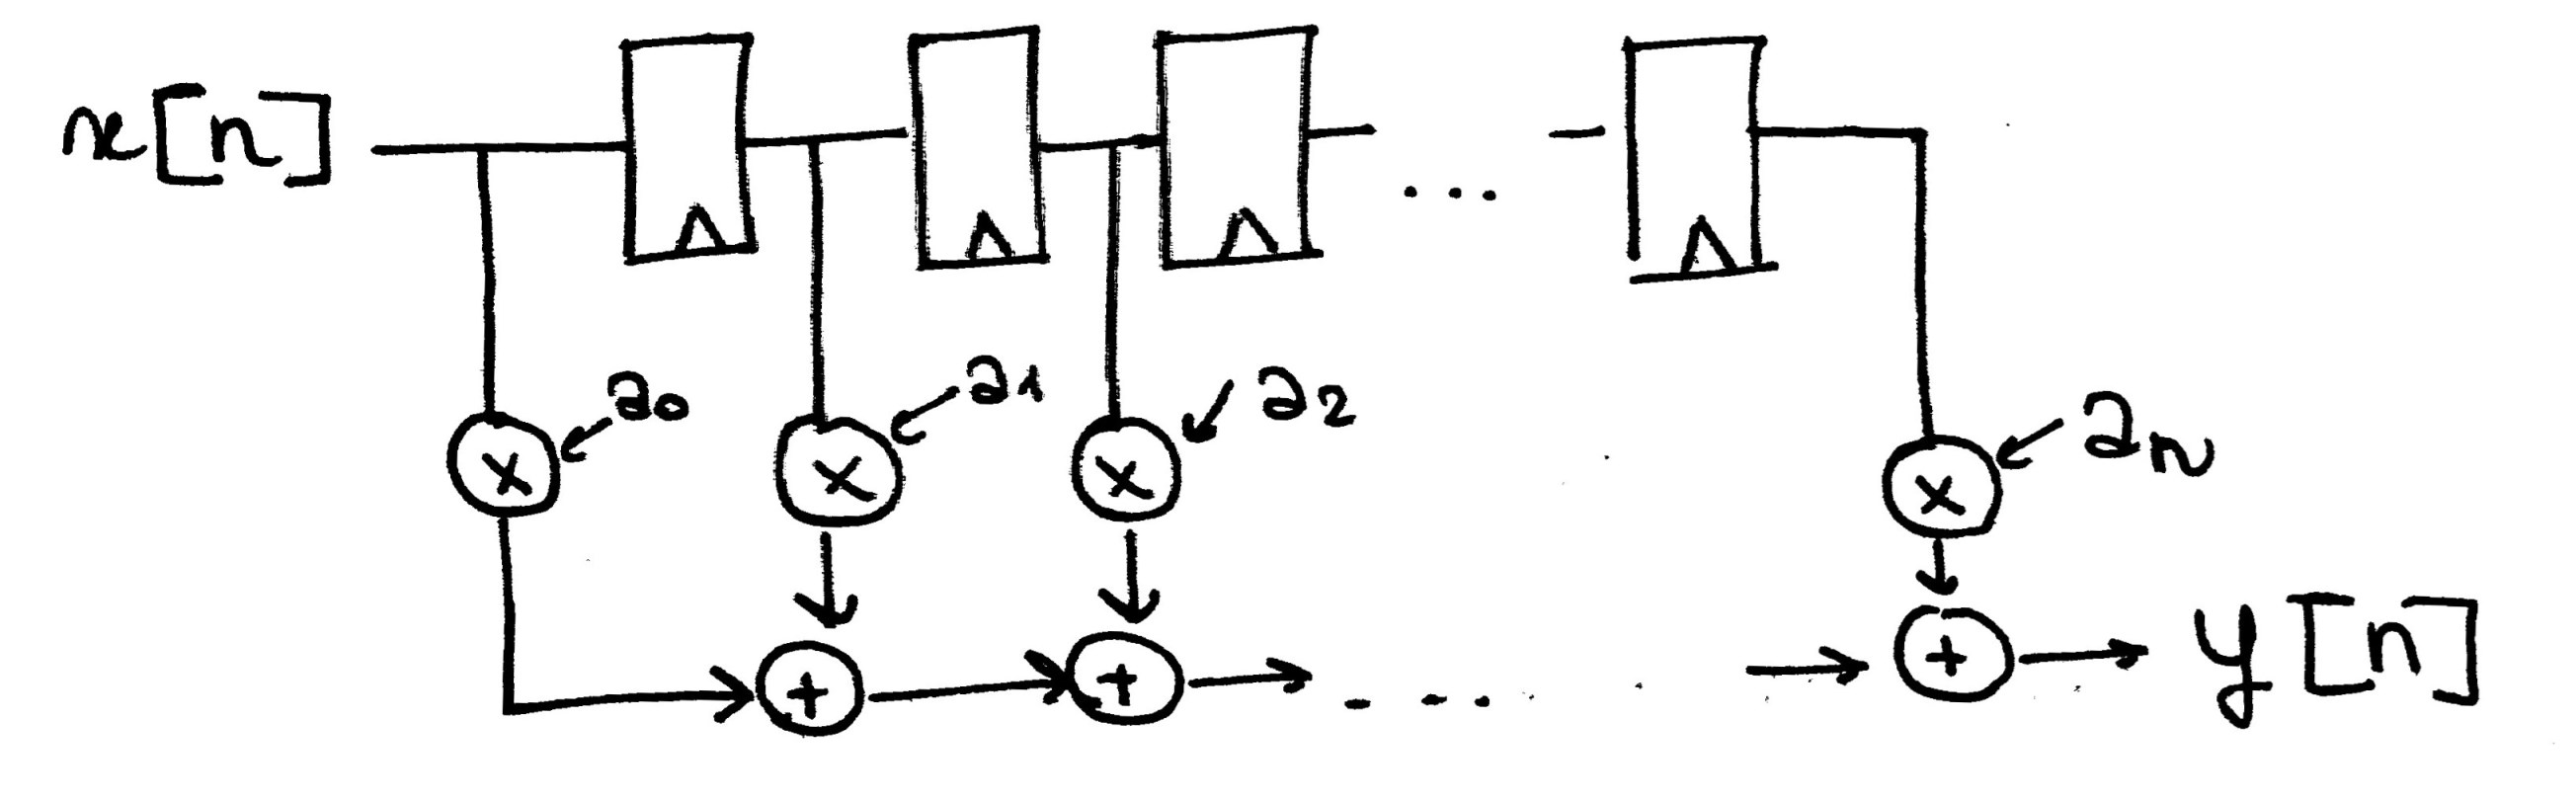
\includegraphics[width=0.7\linewidth]{img/img1/01}
  \captionof{figure}{FIR direct form.}
\end{center}

\begin{center}
  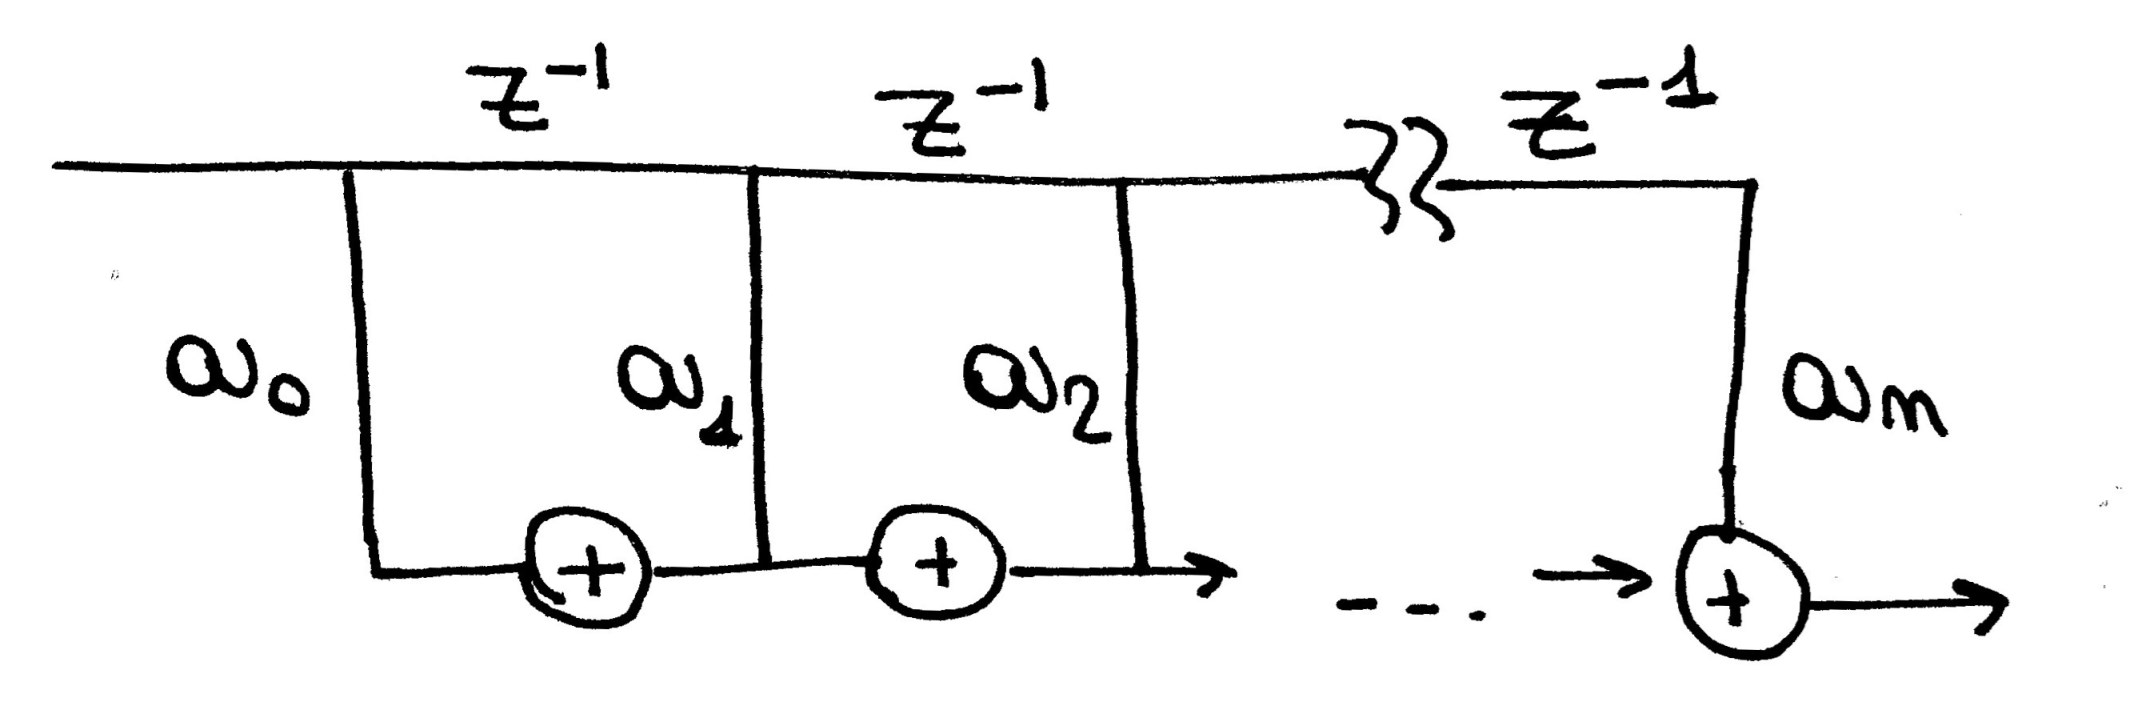
\includegraphics[width=0.7\linewidth]{img/img1/02}
  \captionof{figure}{SFG of same FIR filter.}
\end{center}

In the second figure instead of regs and multipliers, we keep labels on the edges (SFG).

It consists of three elements: adders, multipliers and delayer line. Once we have this flow graph, we can allocate exactly the same hardware or apply pipelining (adding registers) or decrease the complexity (just using one adder and one multiplier). If the main purpose instead is to increase the speed, we can choose a parallel implementation.

Applying some rules, we are able to transform this DFG in a new one.

\subsubsection{Transposed form}

Applying the \textit{transposition theorem}, starting from a graph representing a computational flow, it is possible to obtain a new equivalent DFG by:

\begin{enumerate}
  \item Exchange all edges direction.
  \item Exchange input $\leftrightarrow$ output.
  \item Keep the same gain for every edge (instead of allocate explicitly multipliers, we can refer to SFG representation).
  \item A node that is a fork (i.e. that node replicates its input on two arcs) must be replaced with a new node with 2 inputs and 1 output (due to rule number 1): this means that every fork node must be replace with an adder. Viceversa a summing node in the original graph has to be replaced with a fork node.
  \begin{center}
    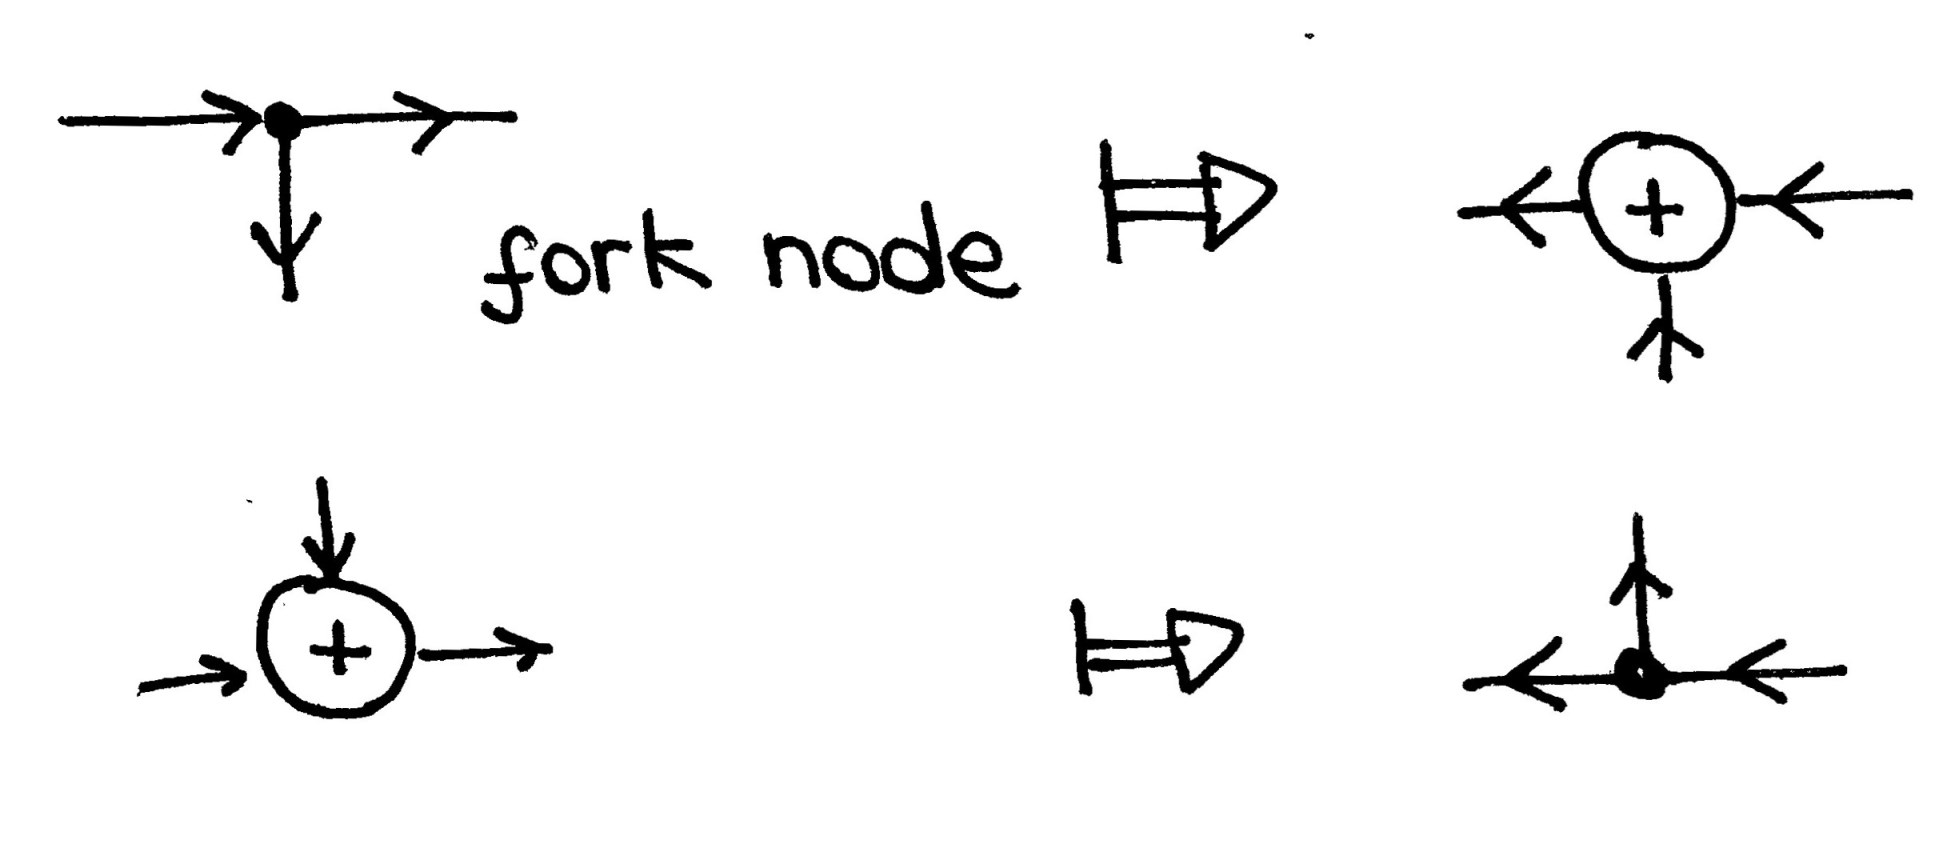
\includegraphics[width=0.7\linewidth]{img/img1/04}
  \end{center}

\end{enumerate}

Applying this theorem to the previous filter:
\begin{center}
  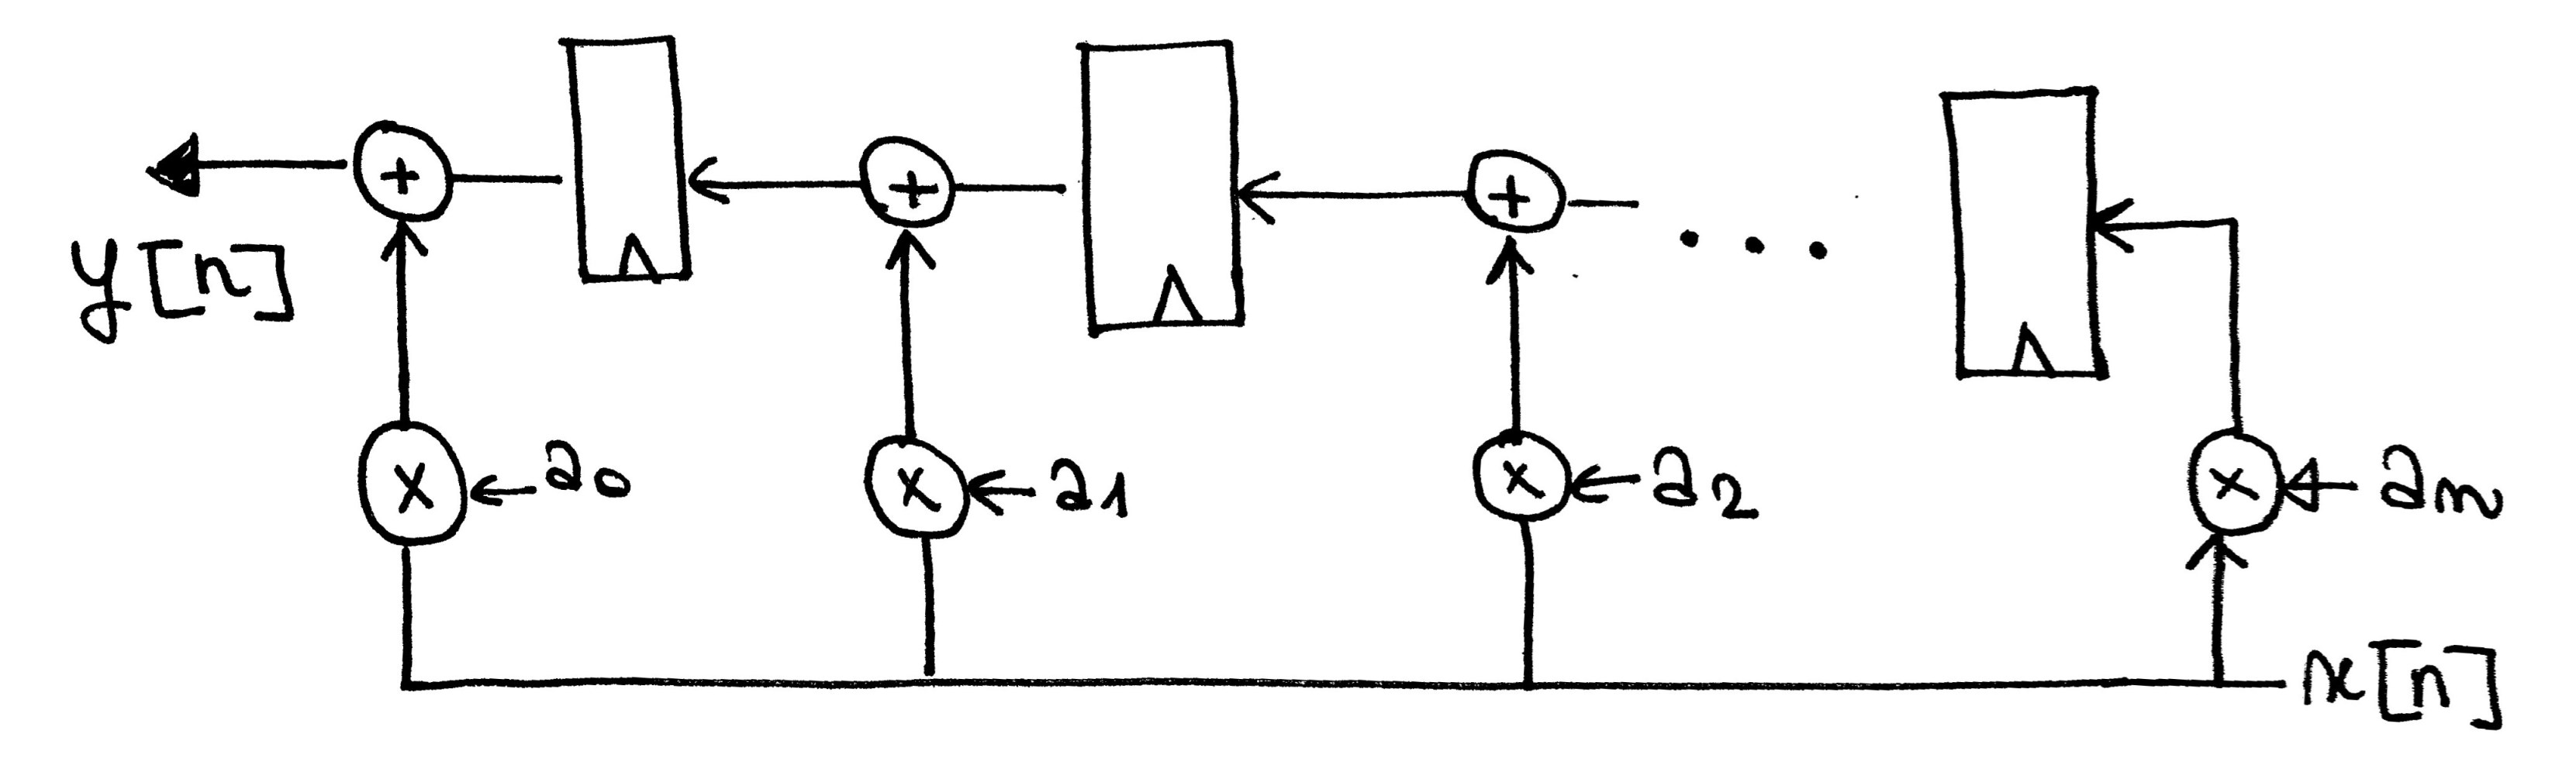
\includegraphics[width=0.7\linewidth]{img/img1/03}
\end{center}

In the transposed form, first we multiply in parallel the input sample for all the coefficients and then we delay it. In order to implement it in hardware, we can decide to apply some techniques like pipelining, etc.

With this representation, the critical path is different since in the direct form it was the one across one multiplier and all the adders (so increasing the filter order it may be a problem) while in the transposed form the critical path is associated to one multiplier and one adder independently on the filter order. It means that probably using transposed form the circuit will have good performance without applying pipelining. \\

One drawback of using transposed form is fanout since it's necessary to apply the same input to many multipliers: in a FPGA this fact can lead to interconnect problems since multiplier blocks may not be near one each other.

\subsubsection{Cascade form}
One of the additional forms for a FIR filter is the cascade. Using Z-transform, we know that:
$$H(z)= \sum_{i=0}^{N} a_i z^{-i} $$

Since it is a polynomial, we can rewrite it using its roots:

$$\sum_{i=0}^{N} a_i z^{-i}= A_0 (1-\frac{z_0}{z}) (1-\frac{z_1}{z})... = A_0 \Pi_{i=0}^{N}(1-\frac{z_i}{z}) $$

In terms of computational structure, it can be seen as:
\begin{center}
  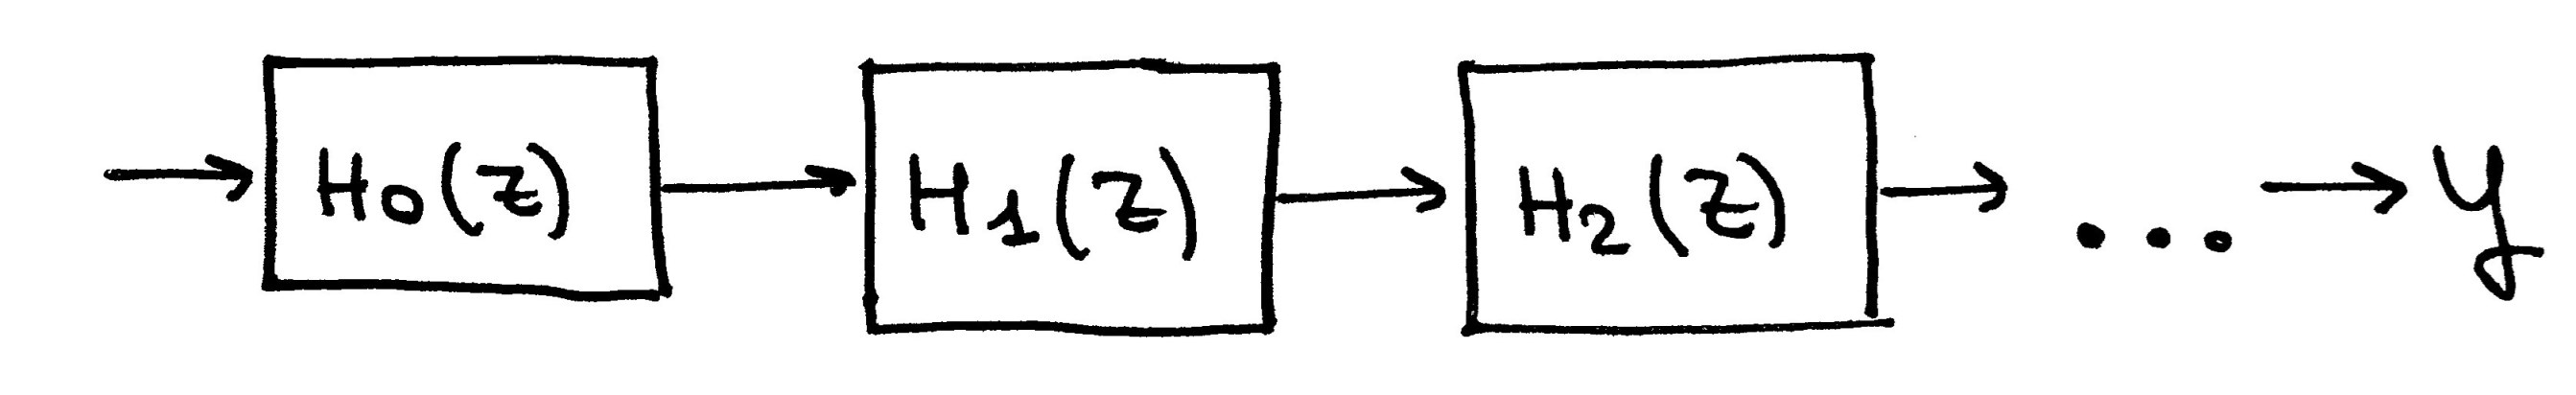
\includegraphics[width=0.7\linewidth]{img/img1/05}
\end{center}

since in Z-tranform the convolution in time is still an algebraic product, the input is passed through many steps where every stage is different from the previous one. For very complex filter, this representation can be employed since it's possible to optimize/tuning each coefficient (or a limited set of them) independently from the others, thus in some way we are applying the divide-et-impera principle.

\subsection{IIR filter implementation}
In general the expression for an IIR filter can be written as:

$$y[n]=\sum_{i=0}^{N} (a_i x[n-i]) + \sum_{j=0}^{M} (b_j y[n-j]) $$

IIR stands for infinite impulse response: we are not able to write the answer to the applied pulses using a limited number of input.

\subsubsection{Direct form I}
Again the first representation is the direct one (just like FIR filters) where the second contribution has been added:

\begin{center}
  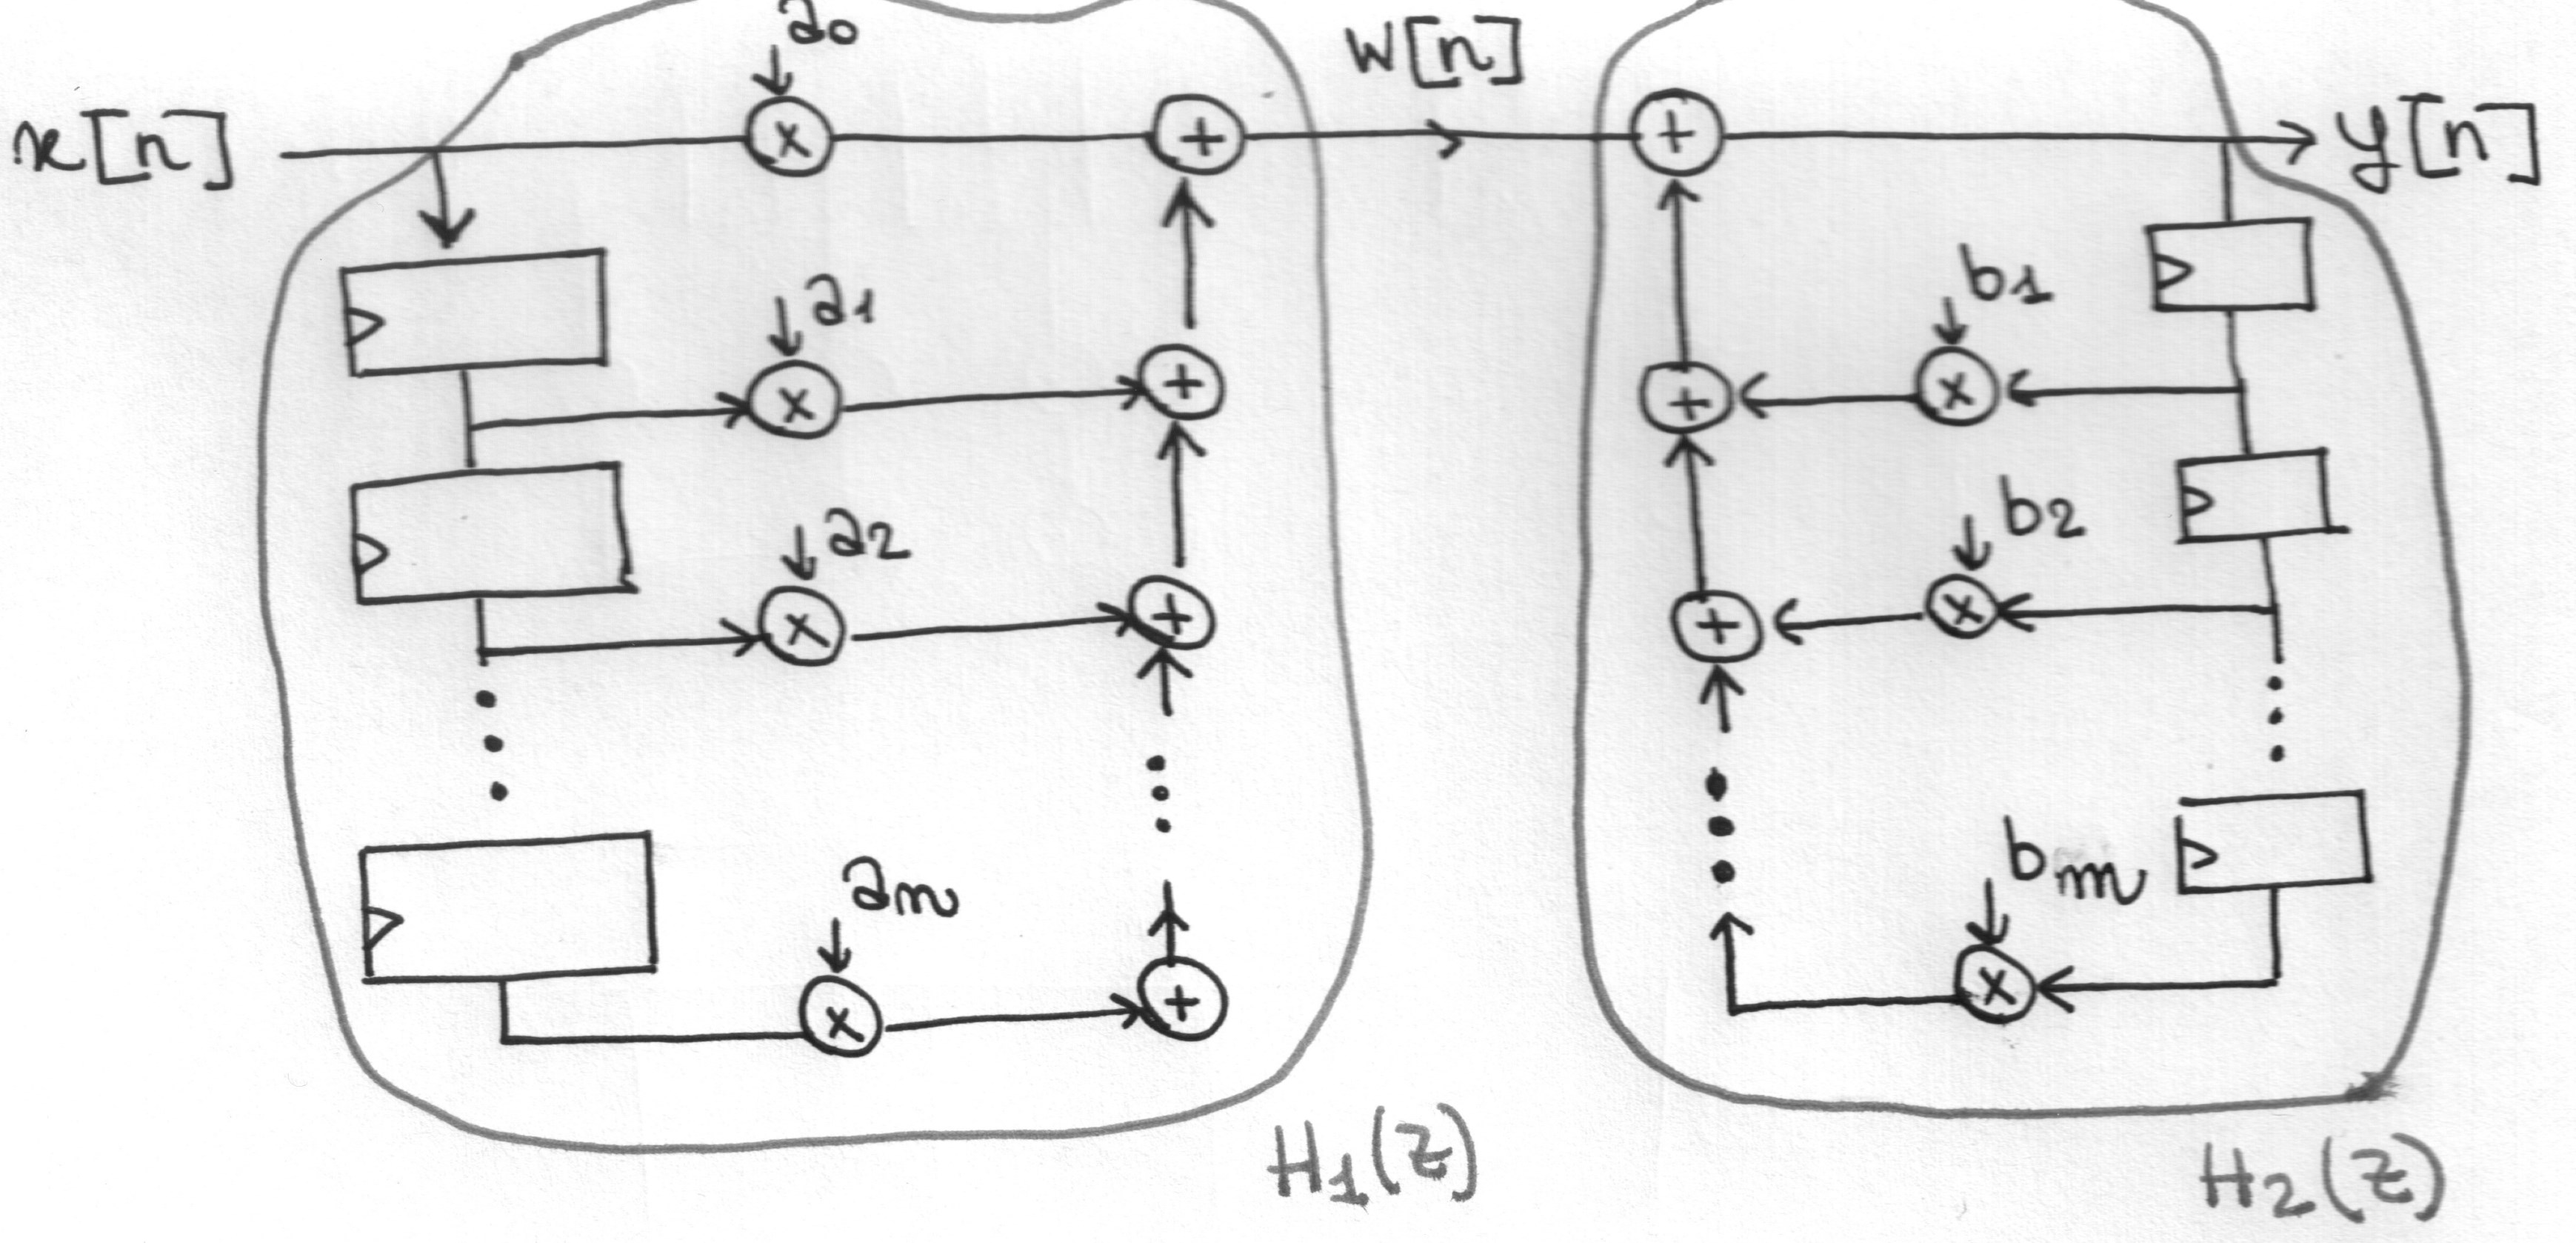
\includegraphics[width=0.7\linewidth]{img/img1/06}
  \captionof{figure}{Direct mapping - direct form I.}
\end{center}

The key differences with respect to FIR filter is that there are loops and that output samples have to been reused. Here we need N+M multipliers, a similar number of adders and two sequences of registers.

\subsubsection{Direct form II}
The first part $x[n] \rightarrow w[n] = H_1(z)$ is just like a FIR filter, while the second part (on the right) has as input $w[n]$ and generates $Y[n]$. This is a cascade of two filters, so the overall response will be $H(z)=H_1(z) \cdot H_2(z)$ (algebraic product). Applying the commutative property, we can exchange $H_1$ and $H_2$. Apparently it's the same, in reality with this transformation we can merge registers saving half of them (resulting in a small device area).
\begin{center}
  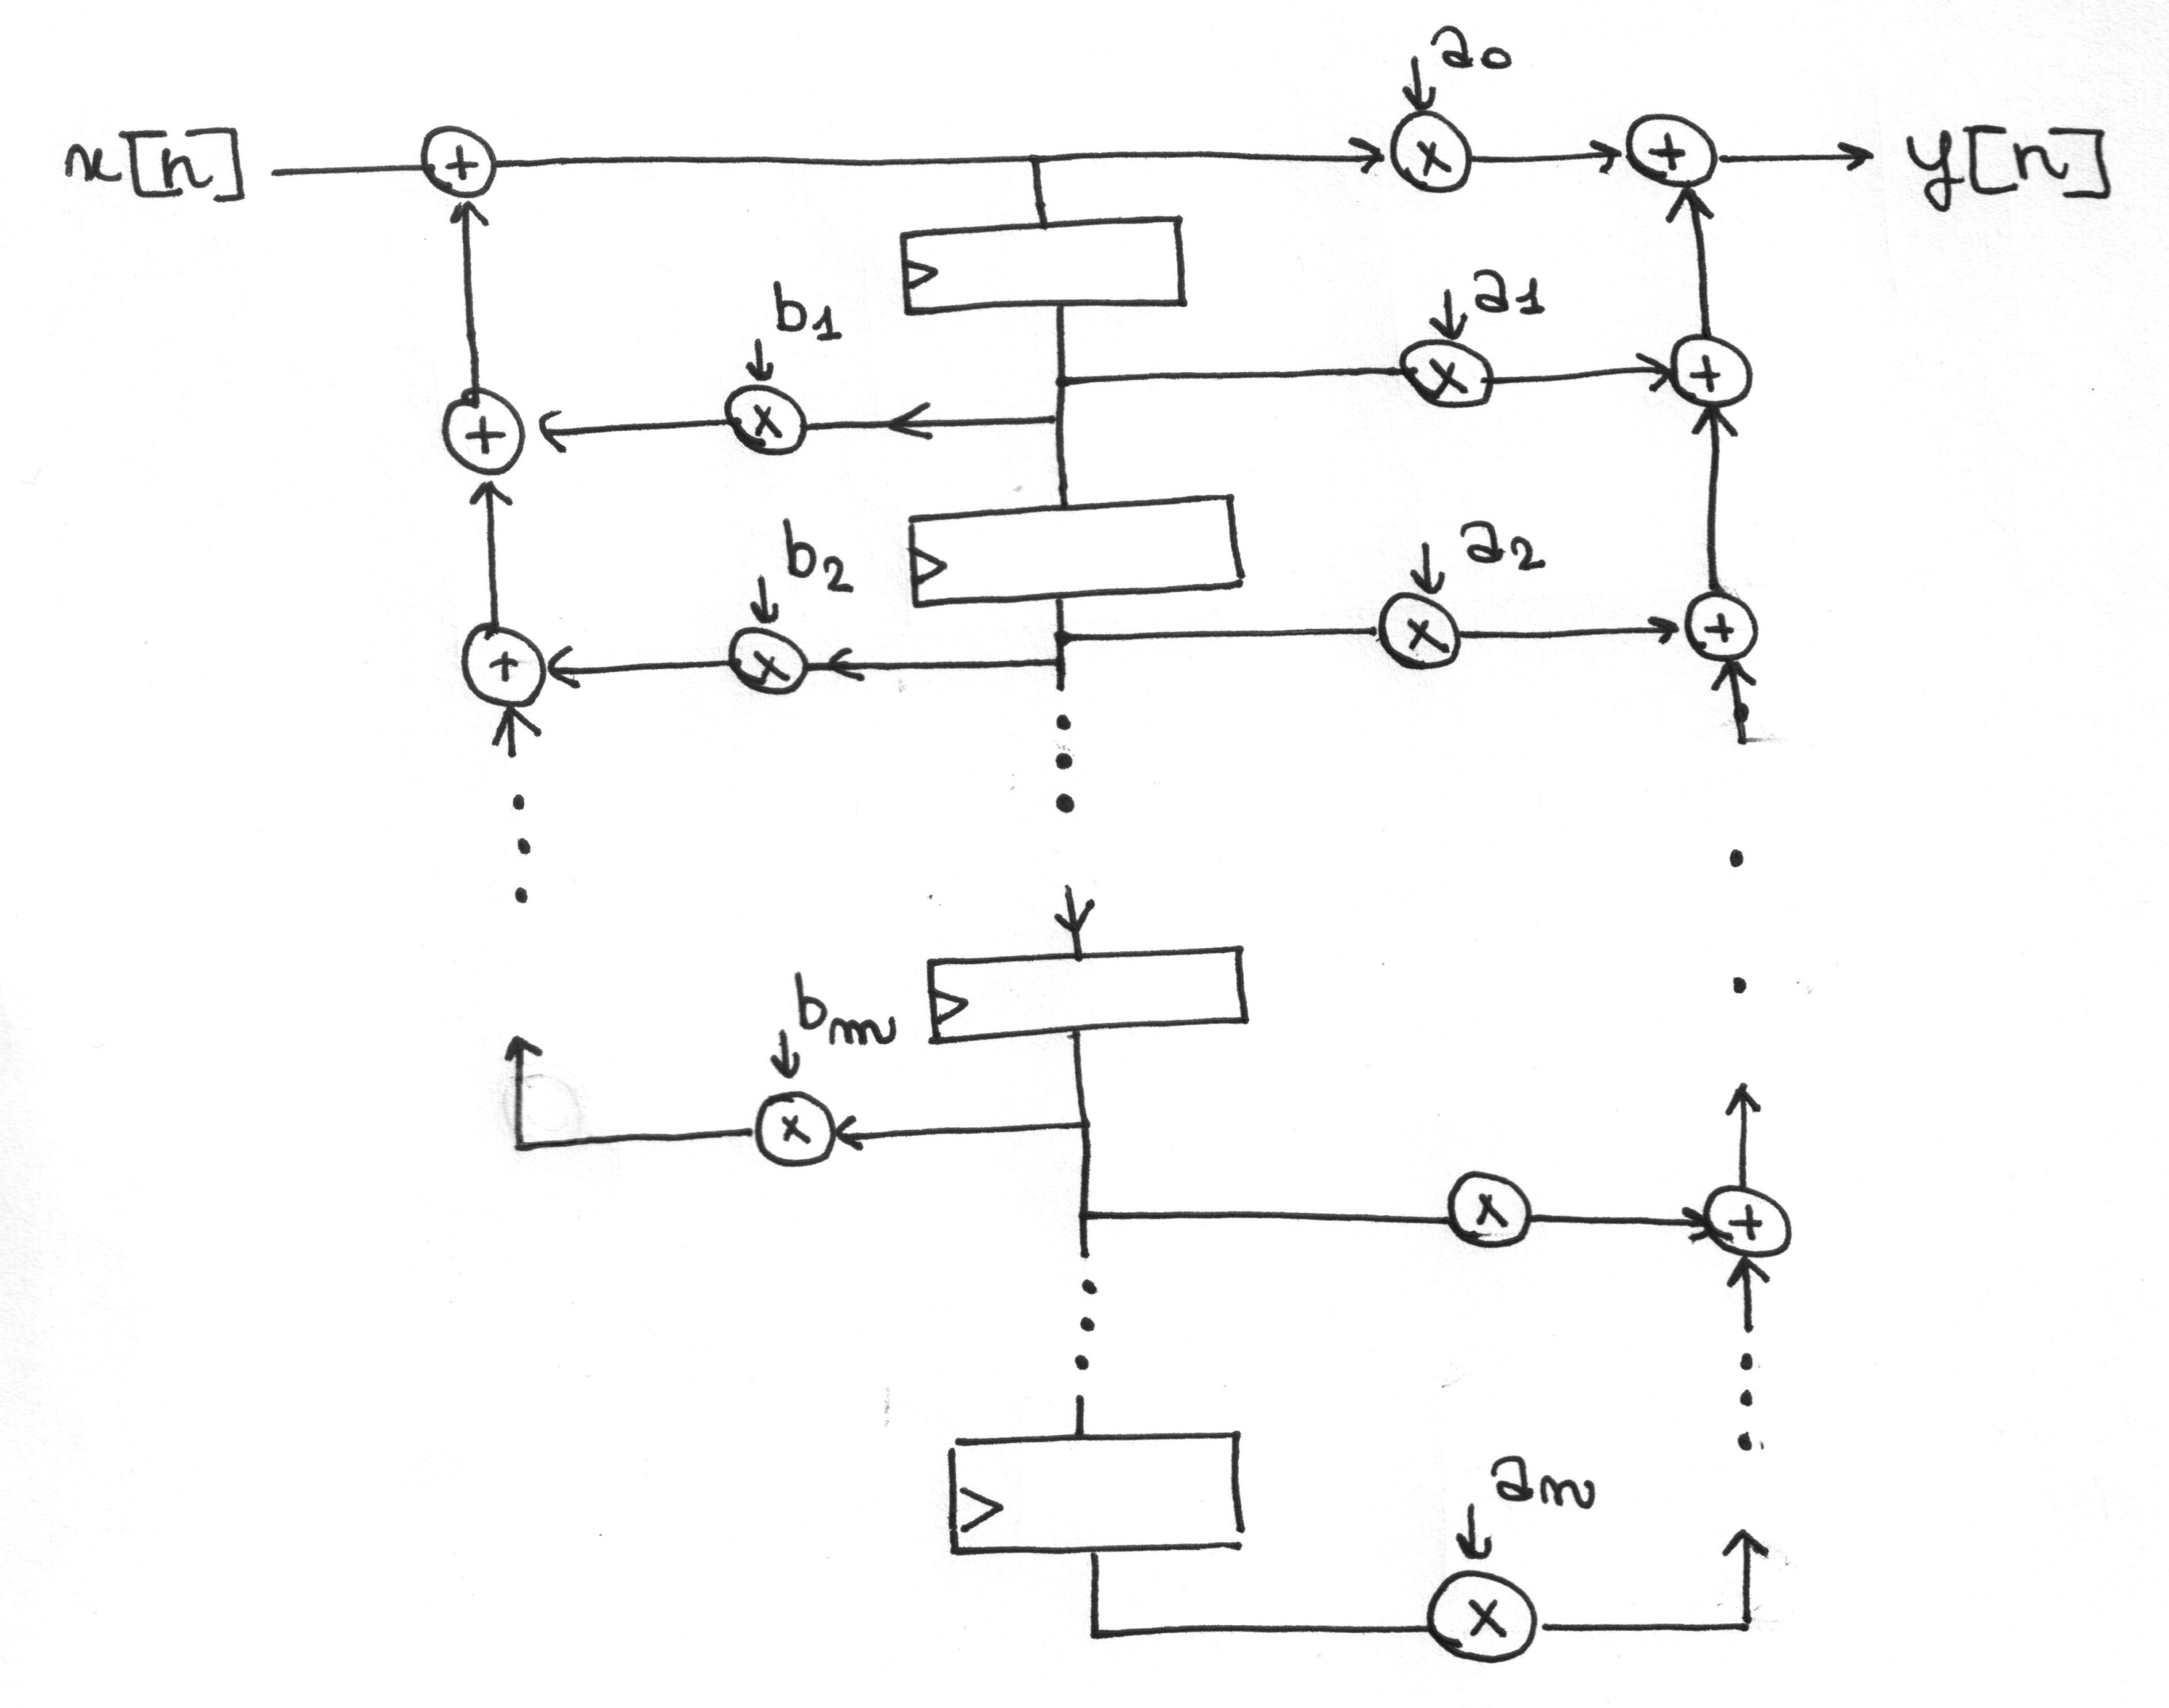
\includegraphics[width=0.7\linewidth]{img/img1/07}
  \captionof{figure}{Direct mapping - direct form II.}
\end{center}

If $N=M$, there is a perfectly overlapping of the two delayer line and the saving of registers is 50\%, otherwise this amount will be lower. In the cascade representation with a degree equal to 2, this representation is often used.
\begin{center}
  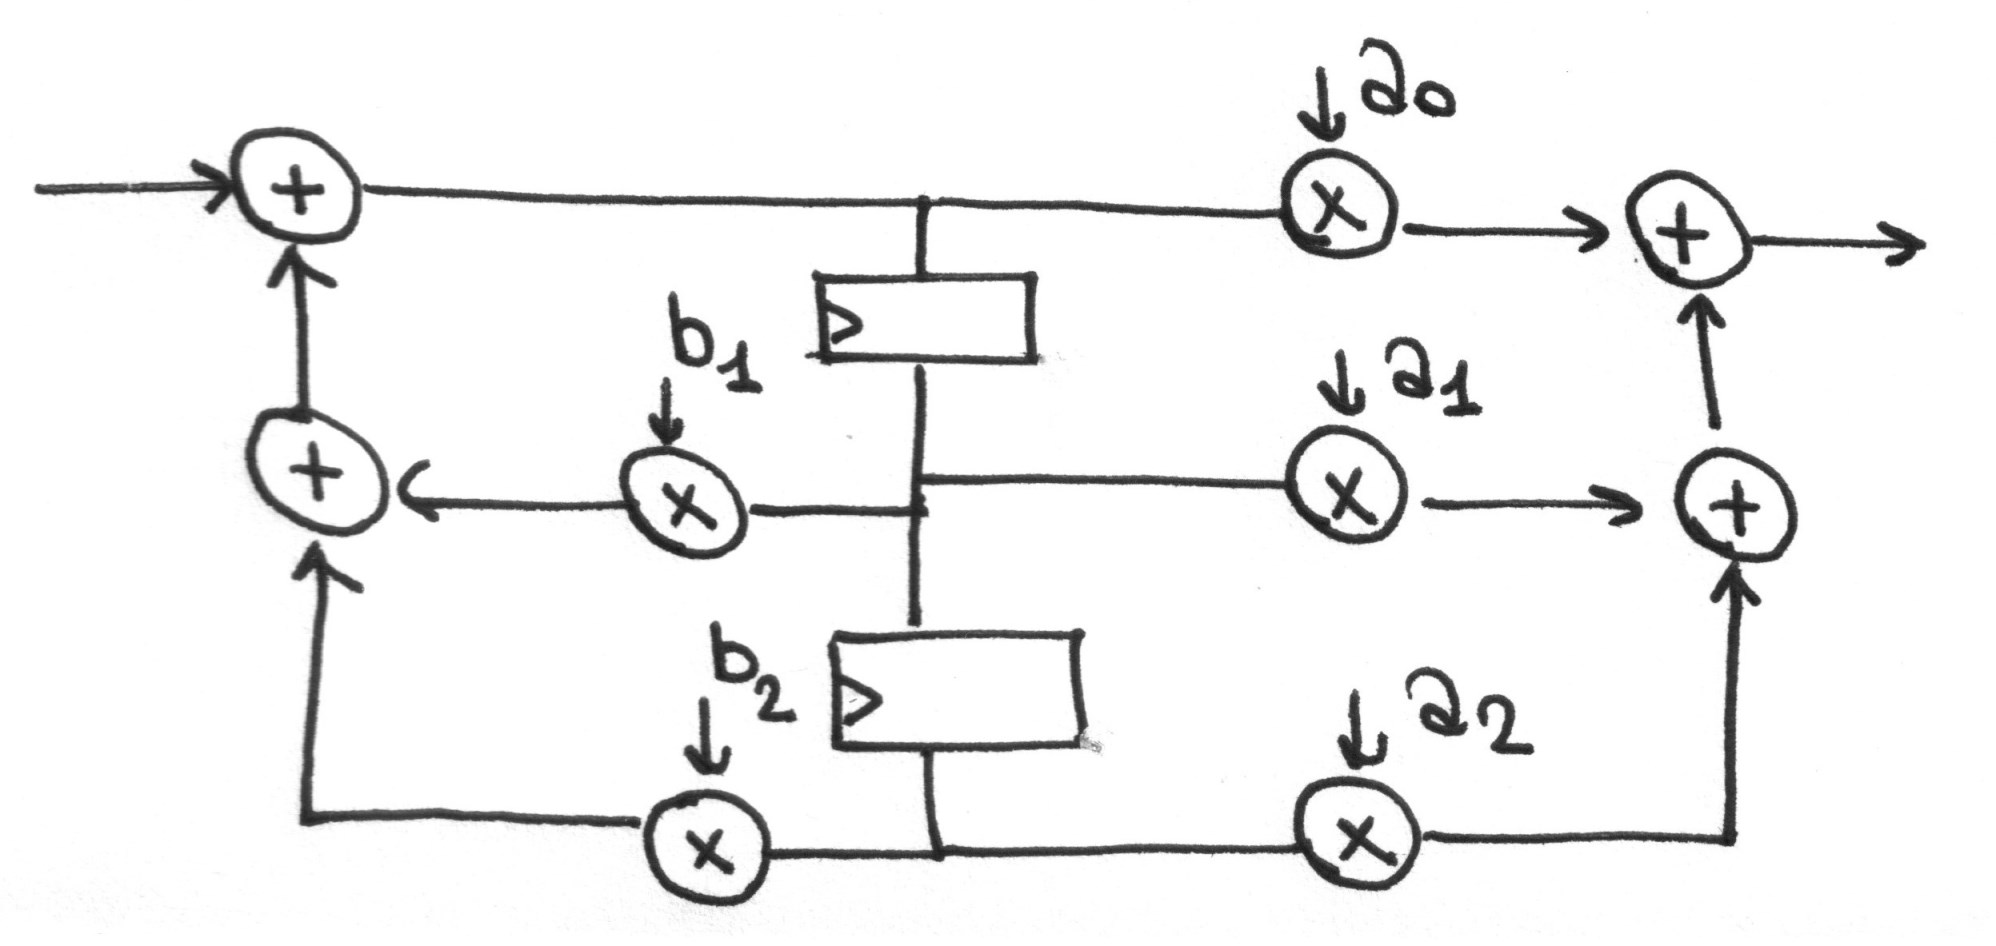
\includegraphics[width=0.7\linewidth]{img/img1/08}
  \captionof{figure}{Second order IIR filter, direct form II.}
\end{center}

In addition there are also all the transposition forms for each of these computational structures (for DF-I, DF-II, cascade).


\section{Filters with loops}
Example where no pipelining can be applied:
\begin{center}
  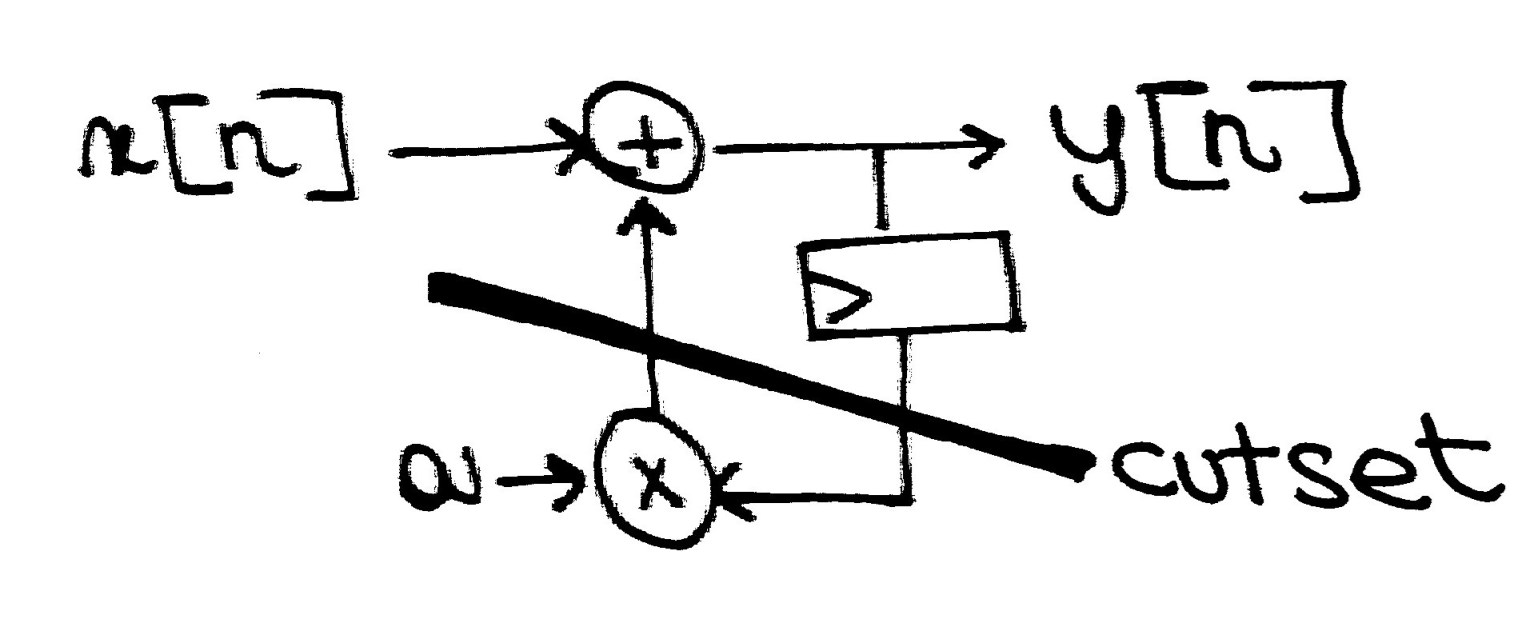
\includegraphics[width=0.6\linewidth]{img/img1/09}
\end{center}

The mathematical expression is:
$$y[n]=x[n]+ay[n-1]$$
The critical path will be $T_{cp}=T_m+T_a$. In order to improve performances, a first idea is to apply pipeline to separate the adder from the multiplier. The point is that, trying to make a cut, the cutset is not feed-forwing since the directions of the arrow are different. So we need other kinds of techniques.

\subsection{Loop bound}
Given a loop, we have the possibility to evaluate the \textbf{loop bound} ($lp$) as the ratio between the total amount of combinational delay and the number of registers/sequential delayer along the loop.\\

Regarding the previous example:

$$ lp= \frac{T_m+T_a}{1} $$

In this particular case we can notice that the loop bound is exactly equal to the critical path delay. It's called \textit{bound} because it is the maximum in term of delay that we can obtain, i.e. we cannot rearrange the loop so that the critical path is smaller than the loop bound. The best implementation therefore is the one for which $T_{cp}=lp$.

If a DFG has more than one loops, we define the \textbf{iteration bound} as the maximum between loop bounds, so in other words:

$$ iteration \hspace{5 pt} bound= max_i (lb_i) $$

\subparagraph{Example}

\begin{center}
  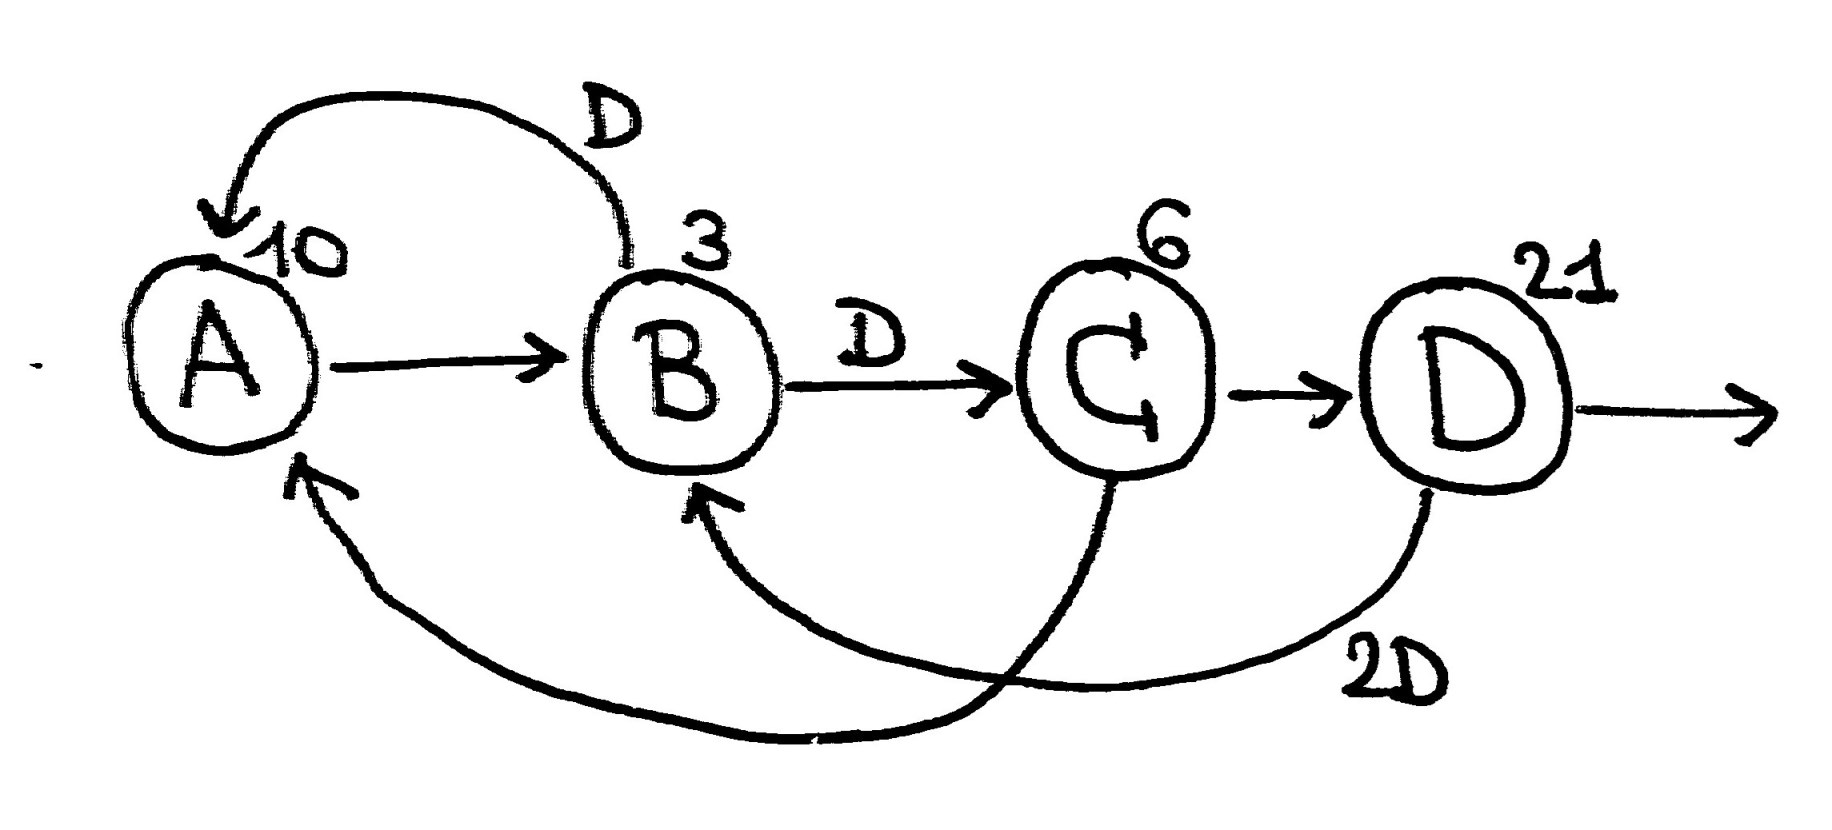
\includegraphics[width=0.6\linewidth]{img/img1/10}
\end{center}

In this example there are three loops, so:

loop 1 (a-b-a): $T_{lb,1}=\frac{10+3}{1}=13$\\
loop 2 (a-b-c-a): $T_{lb,2}=\frac{10+3+6}{1}=19$\\
loop 3 (b-c-d-b): $T_{lb,3}=\frac{3+6+21}{3}=10$\\

iteration bound: $T_{\inf}=max{T_{lb,1},T_{lb,2},T_{lb,3}}=19$\\

Since the critical path delay is equal to 27 and the iteration bound is 19, it means that is possible to improve the performances to make the critical path becoming equal to the iteration bound.

\section{Retiming}
It is the first technique we can apply to a DFG. The key idea is to move the position of registers without affecting the behavior of the algorithm. Retiming can also be applied in order to reduce the number of registers.

\subsection{Solution by inspection}
\begin{center}
  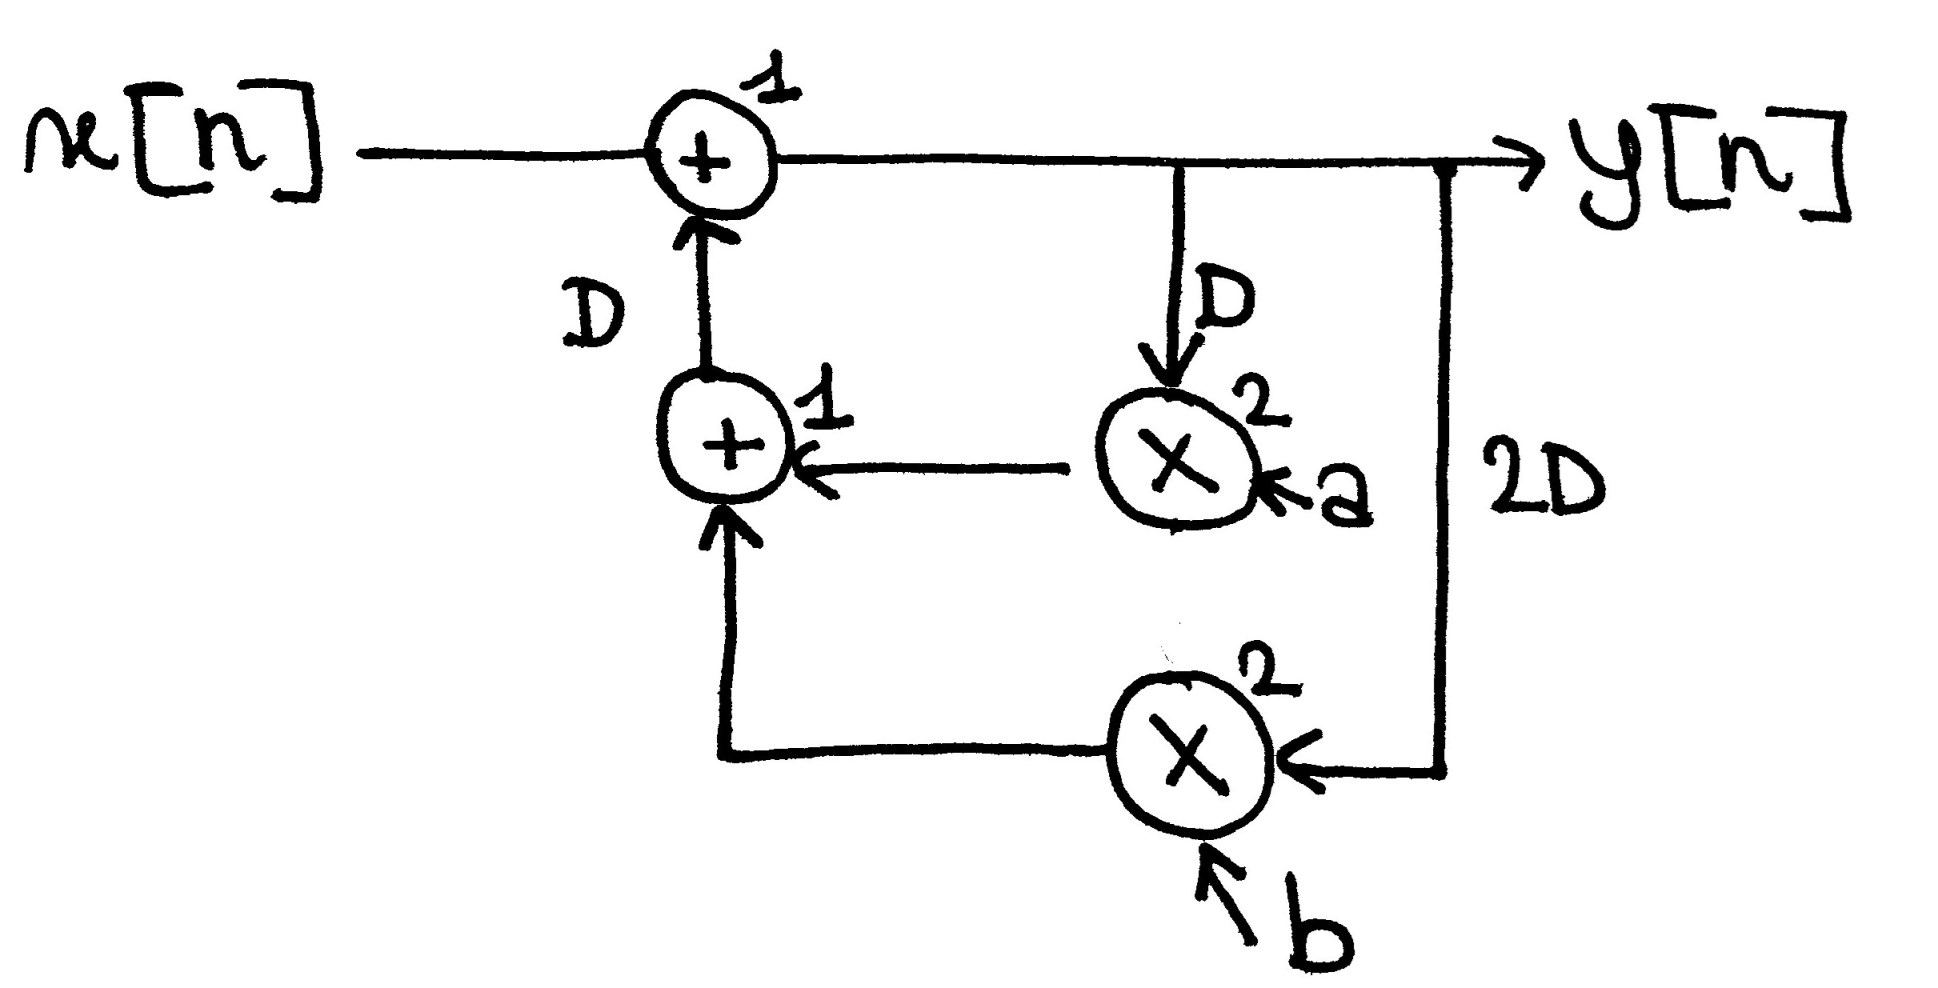
\includegraphics[width=0.6\linewidth]{img/img1/11}
\end{center}

The time discrete representation of this IIR is:
$$y[n]=x[n]+w[n]=x[n]+ay[n-2]+by[n-3]$$

A first approach is to map directly the DFG in an architecture: in this way the critical path will go through one multiplier and one adder ($T_{cp}=T_m+T_a=3$) and the system will generate one output each 3 clock cycles. Since pipelining cannot be implement (no feed-forward cut), we can try to move some registers but before doing it we need to evaluate the iteration loop in order to understand if we can actually improve performances. Since there are one inner loop and one outer loop:
$T_{lb,1}=\frac{4}{2}=2$ (inner loop) \\
$T_{lb,2}=\frac{4}{3}$ (out loop)\\
$T_{\inf}=2 < T_{CP}$

This implies that it makes sense try to speed up the implementation.

By direct inspection, one idea is the following: since the critical path comes from the concatenation of adder and multiplier and between them there is no registers we need to perform in one single cycle 2 operations. We cannot add more registers like in pipeling, the best solution is to move the registers between two adder and moving it back, in this way we obtain $T_{CP}=2$.

\begin{center}
  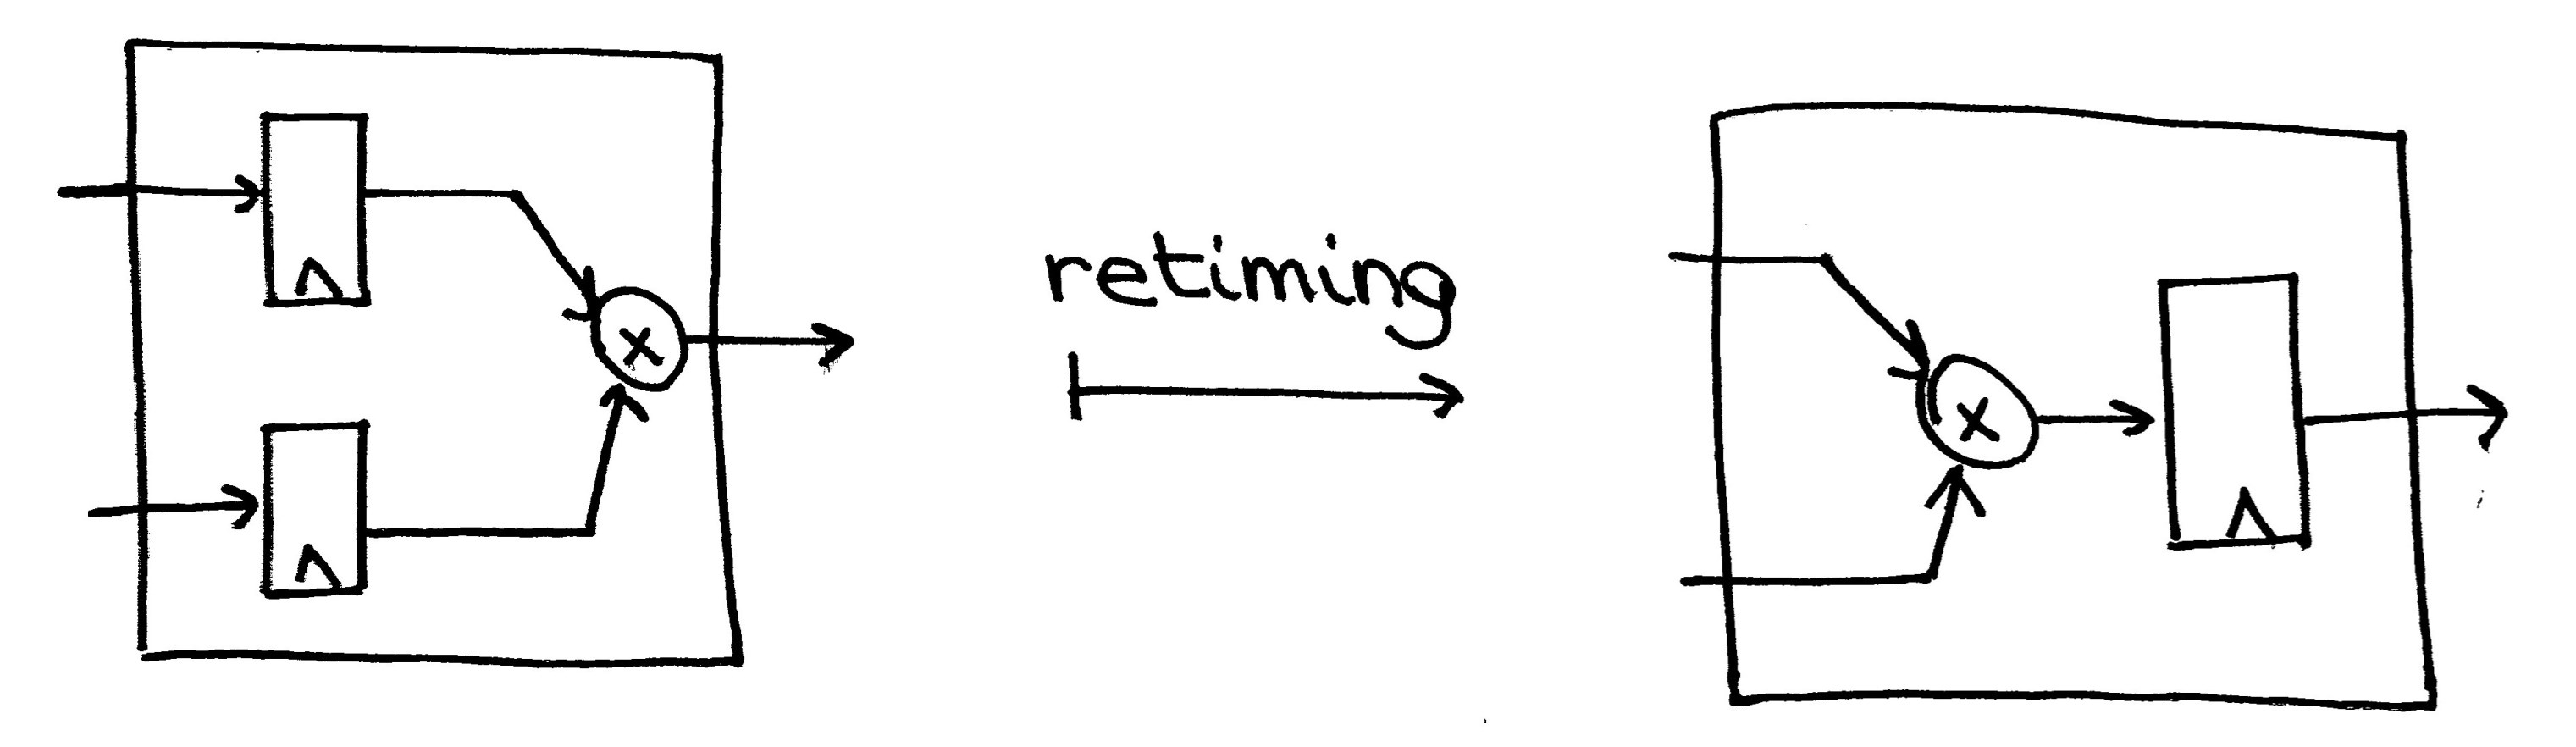
\includegraphics[width=0.7\linewidth]{img/img1/12}
\end{center}

\subsection{Formal method}
Assuming to have one node and some registers, let's call $r(v)$ the number of registers we cancel from the input edge and we move on the output. This amount can also be negative (registers on the output are moved back), the only limitation is not having a negative number of registers.
\begin{center}
  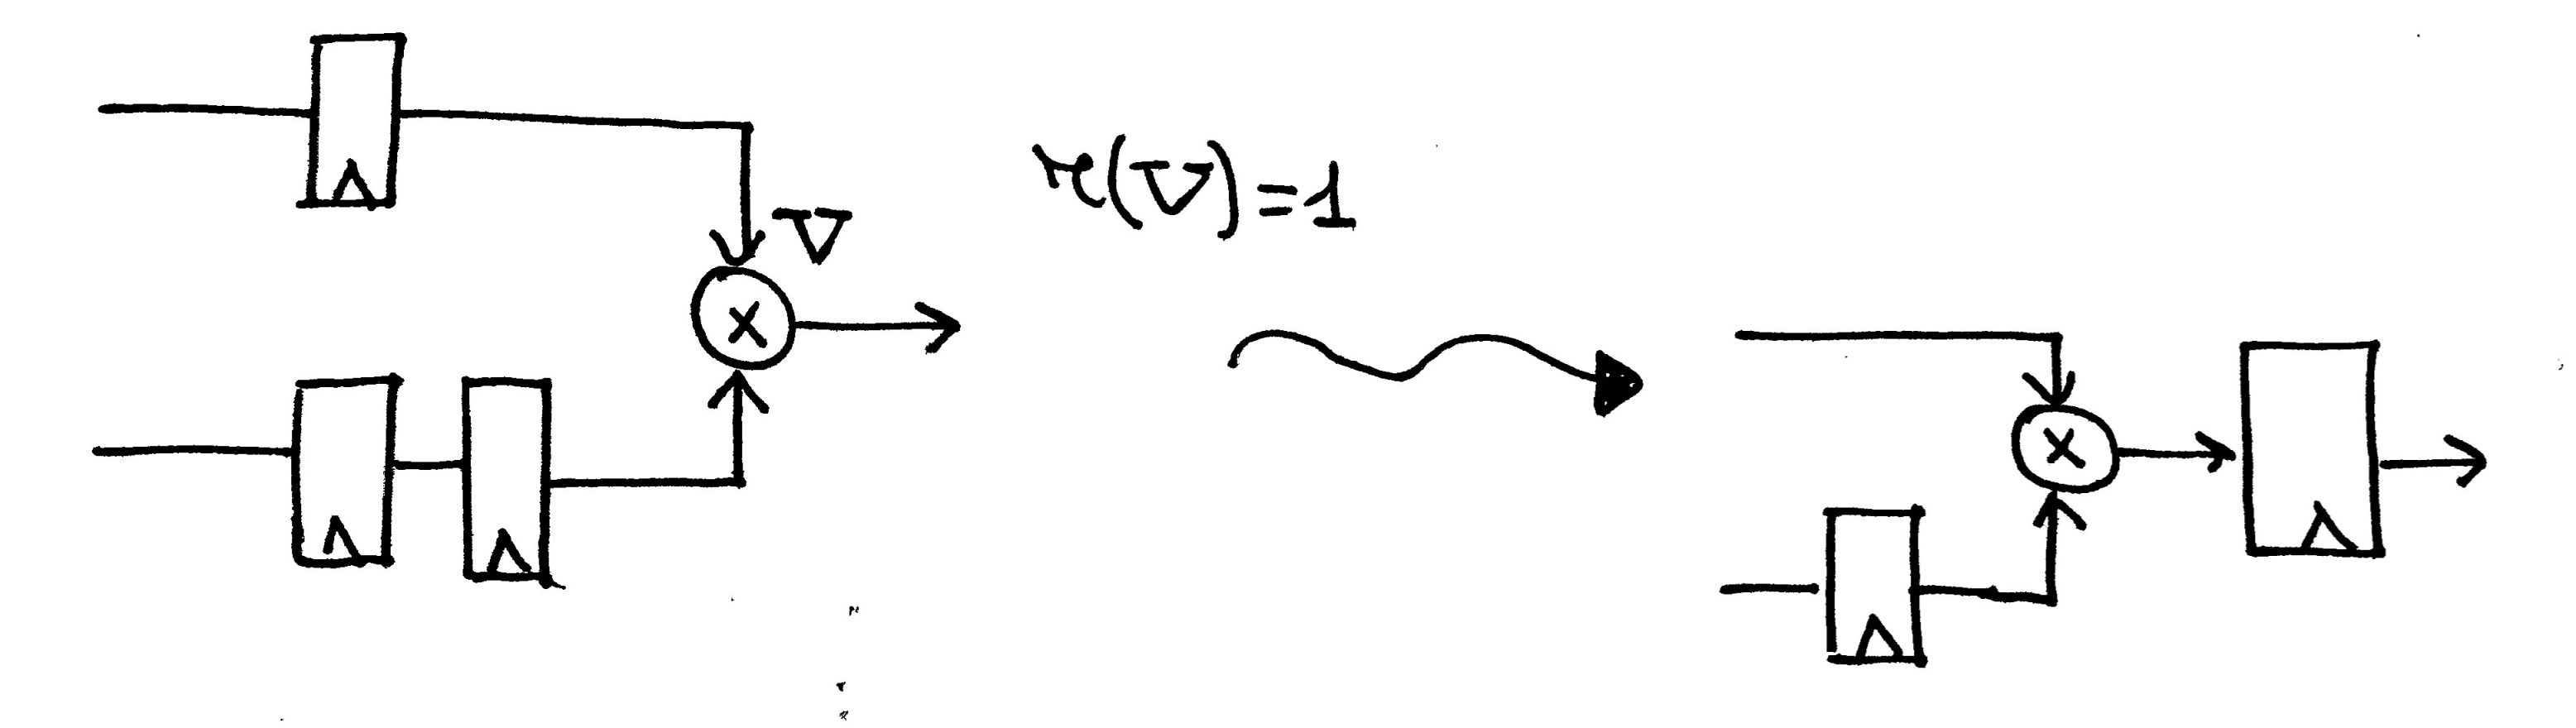
\includegraphics[width=0.7\linewidth]{img/img1/13}
\end{center}

Applying the algorithm to the previous example, we need that all edges satisfy the following condition:
\begin{center}
  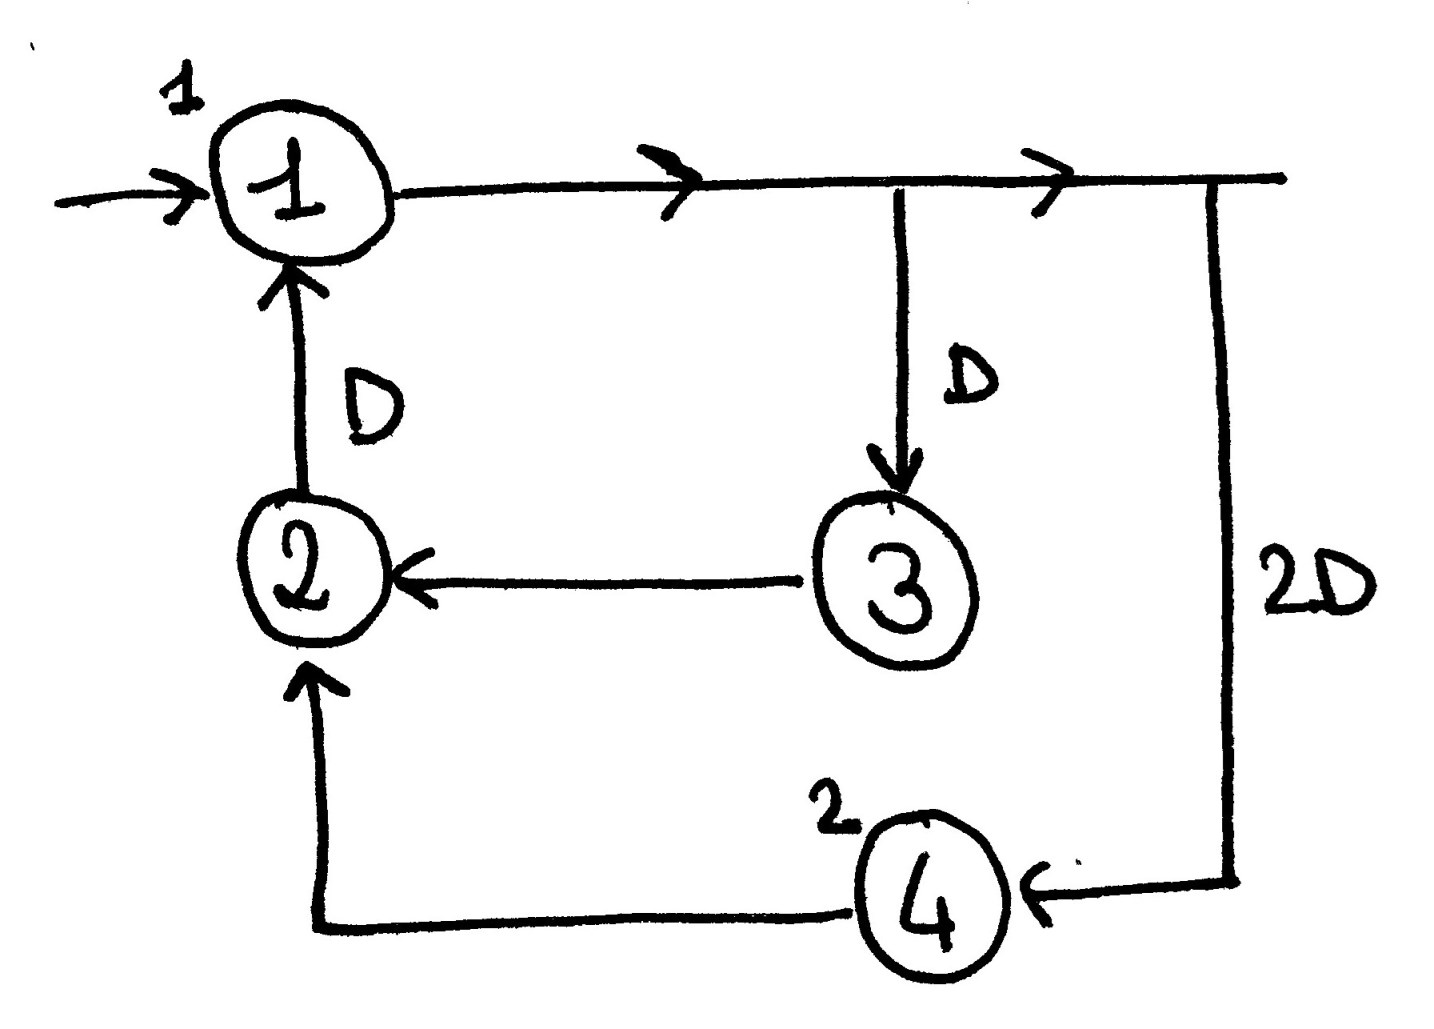
\includegraphics[width=0.5\linewidth]{img/img1/14}
\end{center}
\begin{center}
  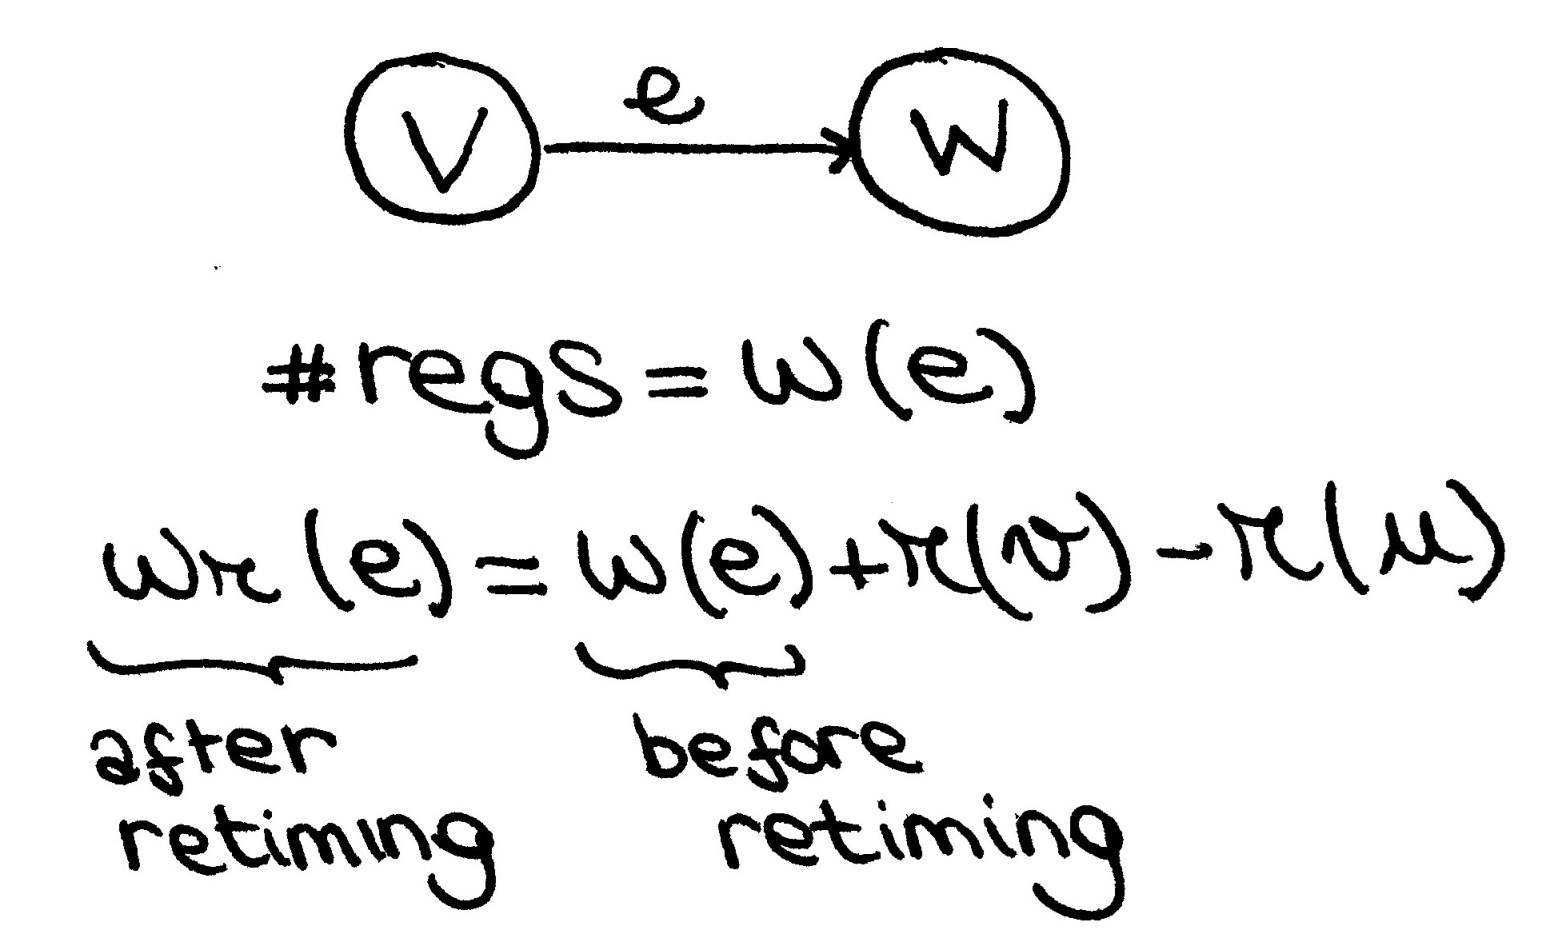
\includegraphics[width=0.5\linewidth]{img/img1/15}
\end{center}

So what we obtain is a set of equations. To find a reasonable solution, we need to set some constrains, like $W_r()<0$ and the fact that we want at least one registers in the edges inside the critical path. Looking at the example:

$$w_r(e_{21}) = w(e_{21}) + r(2) -r(1) \geq 0  \rightarrow 1+r(2)-r(1) >=0$$ (any value of r(2), r(1) is acceptable except not having a negative number of registers)\\
$$w_r(e_{13}) -> 1+r(1)-r(3) >=1 $$ -> not only >=0, but we want to have regs in this subpart 'cause we already know what kind of critical path (separate multipliers from adders).
$$2+r(1)-r(4) >= 1$$
$$0+r(3)-r(2) >= 1$$
$$0+r(4)-r(2) >= 1$$

There are as many equations as many edges on the graph, with certain constrains depending on the fact that the edge is or not inside the critical path. At this point, this comes a mathematical problem that can lead to no solution, one single solution (the ideal case) or many solutions.

One possible solution for the previous set of equations is:
$r(1)=0, r(2)=-1, r(3)=r(4)=0$  that corresponds to the solution found manually.
Another solution is given by:
$r(1)=0, r(2)=-1, r(3)=0 r(4)=1$ that corresponds to the solution by-inspection plus moving one register after multiplier number 4, from the practical point of view nothing changes.\\

\textbf{Issue}: applying retiming $T_{\infty}$ must not change, since it's an intrinsic property of the algorithm . If applying retiming we obtain a different $T_{\infty}$, something is wrong.

\subsection{Cutset retiming}
It is a little easier than the previous method. We need to identify a cutset in the DFG that breaks the critical path and along this cut we're able to perform some modifications.

Taking the same example as before, we already know which are the critical paths. One possibility is to use the shown cutset (it's a cutset since no connections between two subgraphs exists, but it is not a feed-forward one so no pipeling is allowed). Redrawing the DFG after the cut what we obtain is:

Then we add k-registers to every edge from G1 to G2 provided to remove k-registers to every edge from G2 to G1, where k is an integer number greater or lower than zero. While in pipeling we can add as many registers as we want, here if we want to add some registers in the critical path, we need to remove some of them from other path. So applying this method to the previous example, we are able to break the critical path between 2-3. Choosing a different cutset we can obtain the first solution found manually.


\paragraph{Why T infinity is a bound?}
The critical path is defined as $T_{cp}=max(T_a, T_b+T_c)$, i.e. worst case for a specific implementation.
Loop bound is defined as $T_{\infty}=\frac{T_a+T_b+T_c}{2}$ : it means that we can distribute the global computational effort equally in two parts by placing registers exactly in the position required to obtain equal paths.

Assuming $T_a=4$, $T_b=2$, $T_c=4$ then $T_{\infty}=6$ while $T_{cp}=8$: the position of the registers is not the best one since in the first clock cycle we're just doing one operation which is neither the longest one, and in the next clock cycle we're doing two long tasks. The aim is to obtain an equal distribution of computational effort.

There's no guarantee to distribute the computational effort in a uniform way.

\section{Unfolding}
It's also called loop unrolling. to speed up the processing we can unroll the interaction, obtaining multiple interactions executed in a single loop/feedback. In many cases doing this it becomes possible to speed up the processing. These techniques can also be applied to not loop but to feed-forwarding algorithms leading to a parallel implementation.

\subsection{Method I: working on equations}
This is a very simple example, just to see how it works:

\subparagraph{Example I}
\begin{center}
  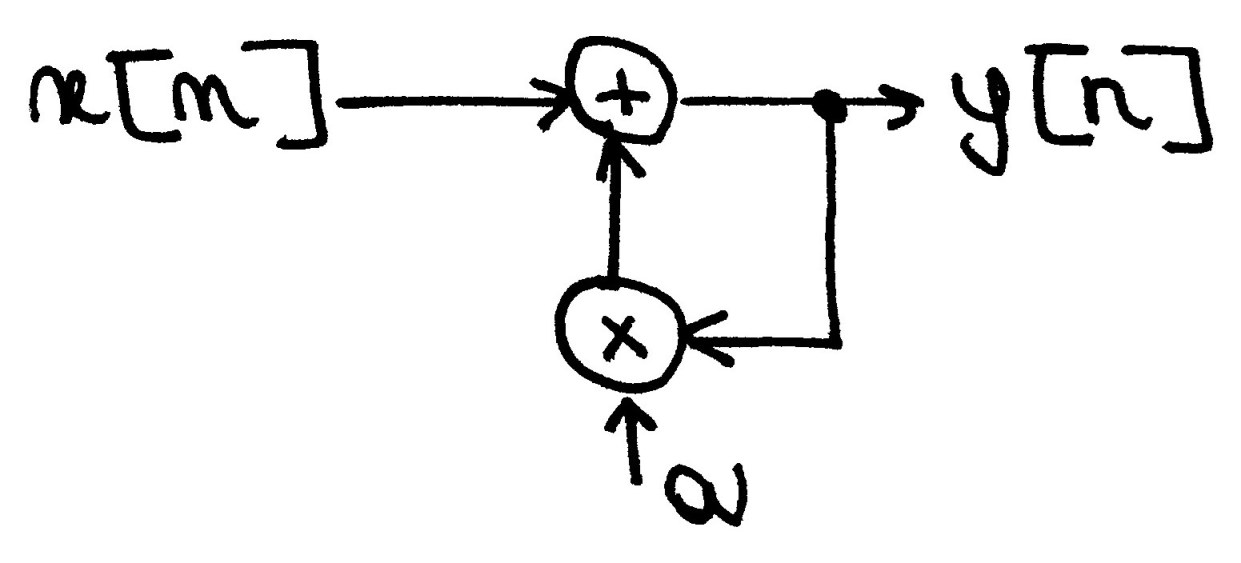
\includegraphics[width=0.6\linewidth]{img/img1/20}
\end{center}

We already know that the filter representation in time domain is the following:
$$y[n]=x[n]+ay[n-1]$$

The key idea is try to unroll it, i.e. apply two interaction at the same time: in order to get this result we cannot anymore use a single input single output system (SISO) but we have to move to a MIMO, meaning that input samples have to be divided into two streams, $x[2k]$ and $x[2k+1]$. Therefore we expect to produce also two output at the same time. Starting from the original representation and substituting index $n$ with $2k, 2k+1$ what we get is:
\begin{eqnarray}
y[2k]=x[2k]+ay[2k-1]\\
y[2k+1]=x[2k+1]+ay[2k]
\end{eqnarray}

Map it directly in hardware leads to:

\begin{center}
  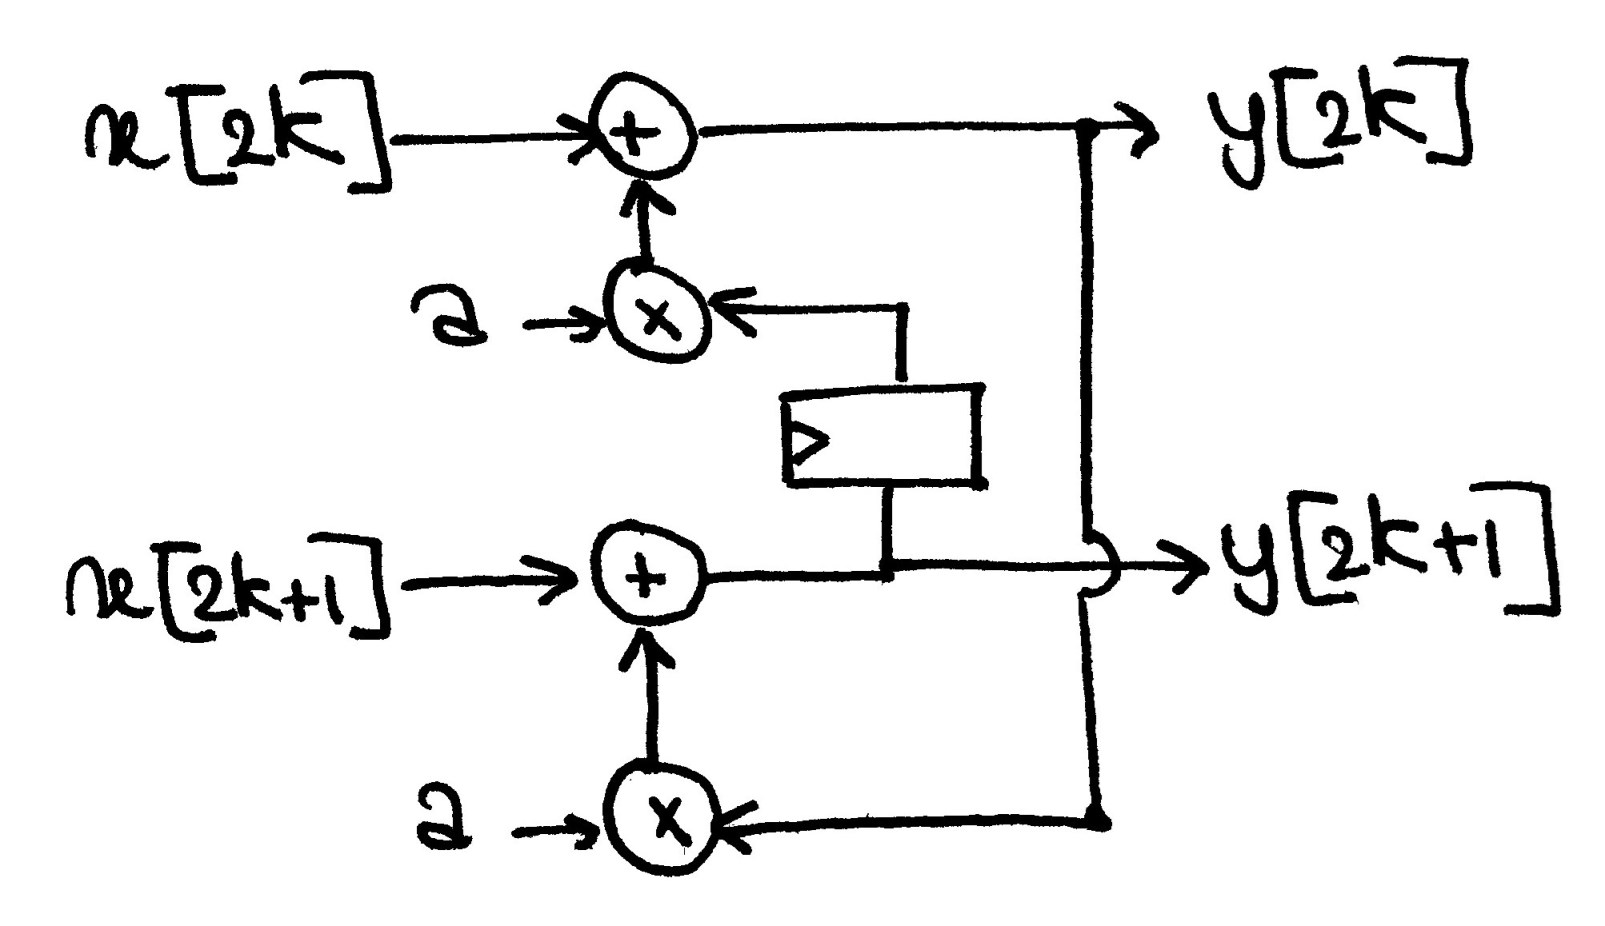
\includegraphics[width=0.6\linewidth]{img/img1/21}
\end{center}

\textbf{Warning}: we only need a register (and not two) for the first stream, while for the second we don't need any delayer.\\
This parallel implementation is not a simply replication of the previous DFG but there's a mixing between signals. To not produce any error, we need to adopt a method. In this case we use the first method which consists of working on equations, obtaining a new representation and then mapping it in a new DFG. Another method allow us to work directly on DFG.

\subparagraph{Example II}

Let's apply the same method (the one with equations) to a little more complicated filter:

\begin{center}
  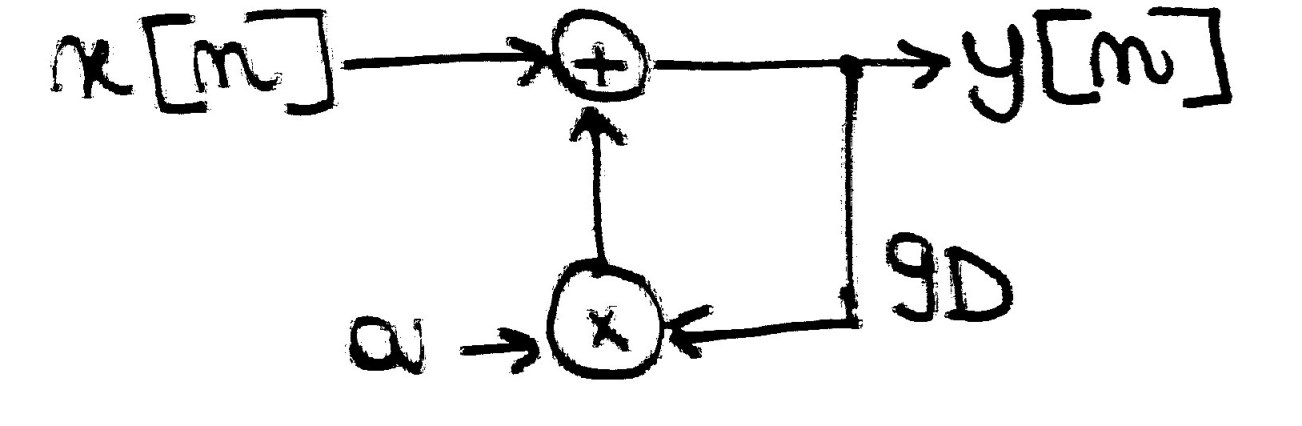
\includegraphics[width=0.6\linewidth]{img/img1/22}
\end{center}

Now the starting point is:
\begin{equation}
y[n]=x[n]+ay[n-9]
\end{equation}

Again we want to instantiate two streams working in parallel:
\begin{eqnarray}
y[2k]=x[2k]+ay[2k-9];     \\
y[2k+1]=x[2k+1]+ay[2k-8];
\end{eqnarray}

In order to map these equations in hardware, we first need to determine the number of delayers to be inserted. Looking at the equation is not so clear. Rewriting the second equation we understand that we need an even sample delayed of 4 steps. Similarly for the first one:
\begin{equation}
y[2k+1]=x[2k+1]+ay[2(k-4)] \\
y[2k]=x[2k]+ay[2(k-5)+1]
\end{equation}

\begin{center}
  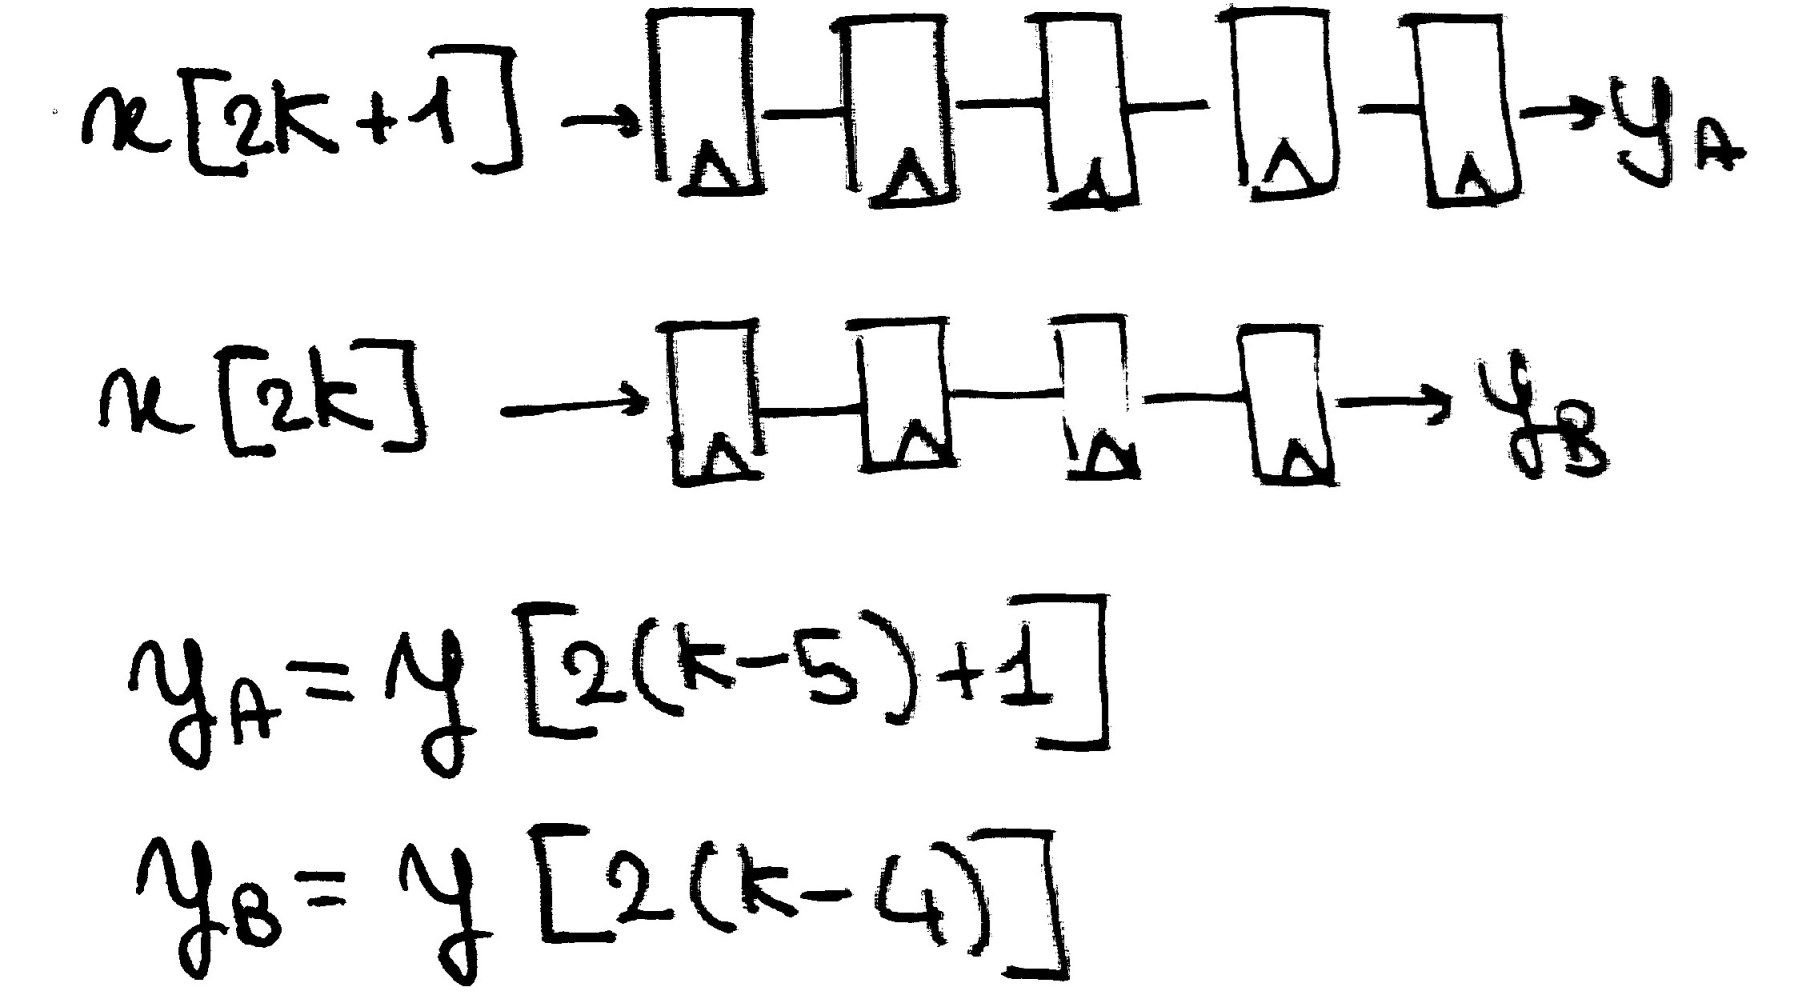
\includegraphics[width=0.6\linewidth]{img/img1/23}
\end{center}

So instead of working with $n$, it's better to deal with index $k$, that is already splitted for two instances. Now we can draw the new DFG like:

\begin{center}
  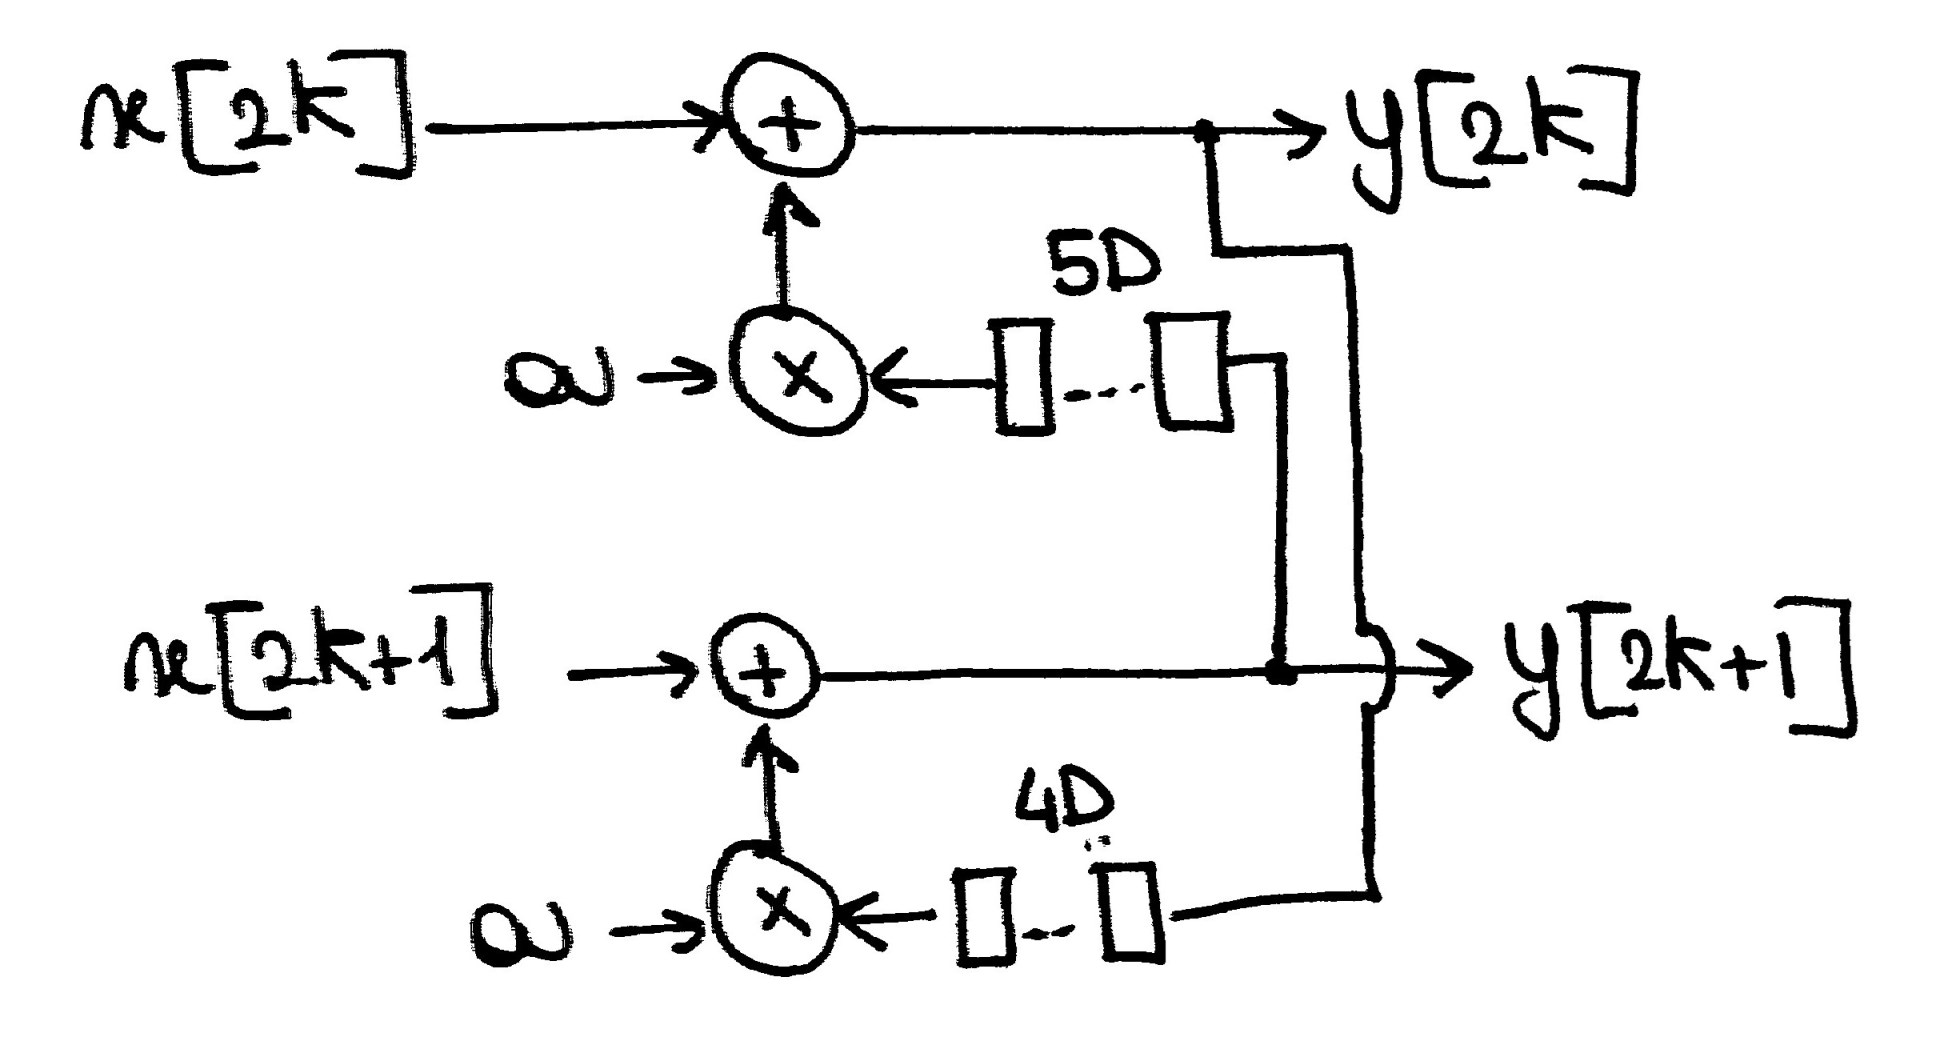
\includegraphics[width=0.6\linewidth]{img/img1/24}
\end{center}

Looking at the performance of the original DFG (the one with 9D):
\begin{eqnarray}
T_{cp}=T_a+T_m=1+3=4\\
th=\frac{1}{4}\\
T_{\infty}=\frac{T_a+T_m}{9}=\frac{4}{9}
\end{eqnarray}

It means that the original architecture can be improved, so we try to apply unfolding. After that, performances become:
\begin{eqnarray}
T_{cp}=T_a+T_m=4\\
th=\frac{2}{T_a+T_m}=\frac{1}{2}\\
\end{eqnarray}
Where $th$ (throughput) is defined as the amount of samples we are able to produce per unit time, since $T_{clk}$ is determined by $T_{cp}$, it will be the same as before (we don't increase clock frequency) but $th$ doubles because it's no more a SISO but it's a MIMO system.

Increasing the degree of parallelism, speed up factor will be 3 instead of 2 (ideally). Can we increase the throughput with no limit? We expect a saturation not only because we are adding registers, but also due to $T_{\infty}$, so it makes sense increase the parallelism of the architecture until reaching $T_{\infty}$. This is why is so important evaluate this parameter before starting an optimization.

\subparagraph{Example: degree of parallelism equals to 3}

It's straightforward derive the new equations for a degree od parallelism equal to 3, it's only a matter of replacing index $n$ with $3k, 3k+1, 3k+2$:
\begin{eqnarray}
y[3k]=x[3k]+ay[3k-1];\\
y[3k+1]=x[3k+1]+ay[3k];\\
y[3k+2]=x[3k+2]+ay[3k+1];
\end{eqnarray}

\subsection{Method II: working on DFG}

Starting from an original DFG, we want to map it to an unfolded DFG (called DFG') applying a degree of unfolding equal to J. The required steps are:
\begin{enumerate}
  \item For every node in DFG, allocate J nodes of the same type, called $u_0$, $u_1$...$u_{J-1}$.
% \item For every edge in DFG, $e: u  \overset{w}{\rightarrow} v$ (stands for edge $e$ connecting node $u$ with $v$ with $w$ delayer), allocate J edges (one for each replica of $u$) $e_j: u_i \overset{w_i}{\rightarrow} V_j$ where $j=\frac{i+w}{J}\% J$ and along this new edge we have to place $w_i$ delayer with $i= \integer{\frac{i+w}{J}}$.
\end{enumerate}

\subparagraph{Example: the previous one with 9D}

\begin{center}
  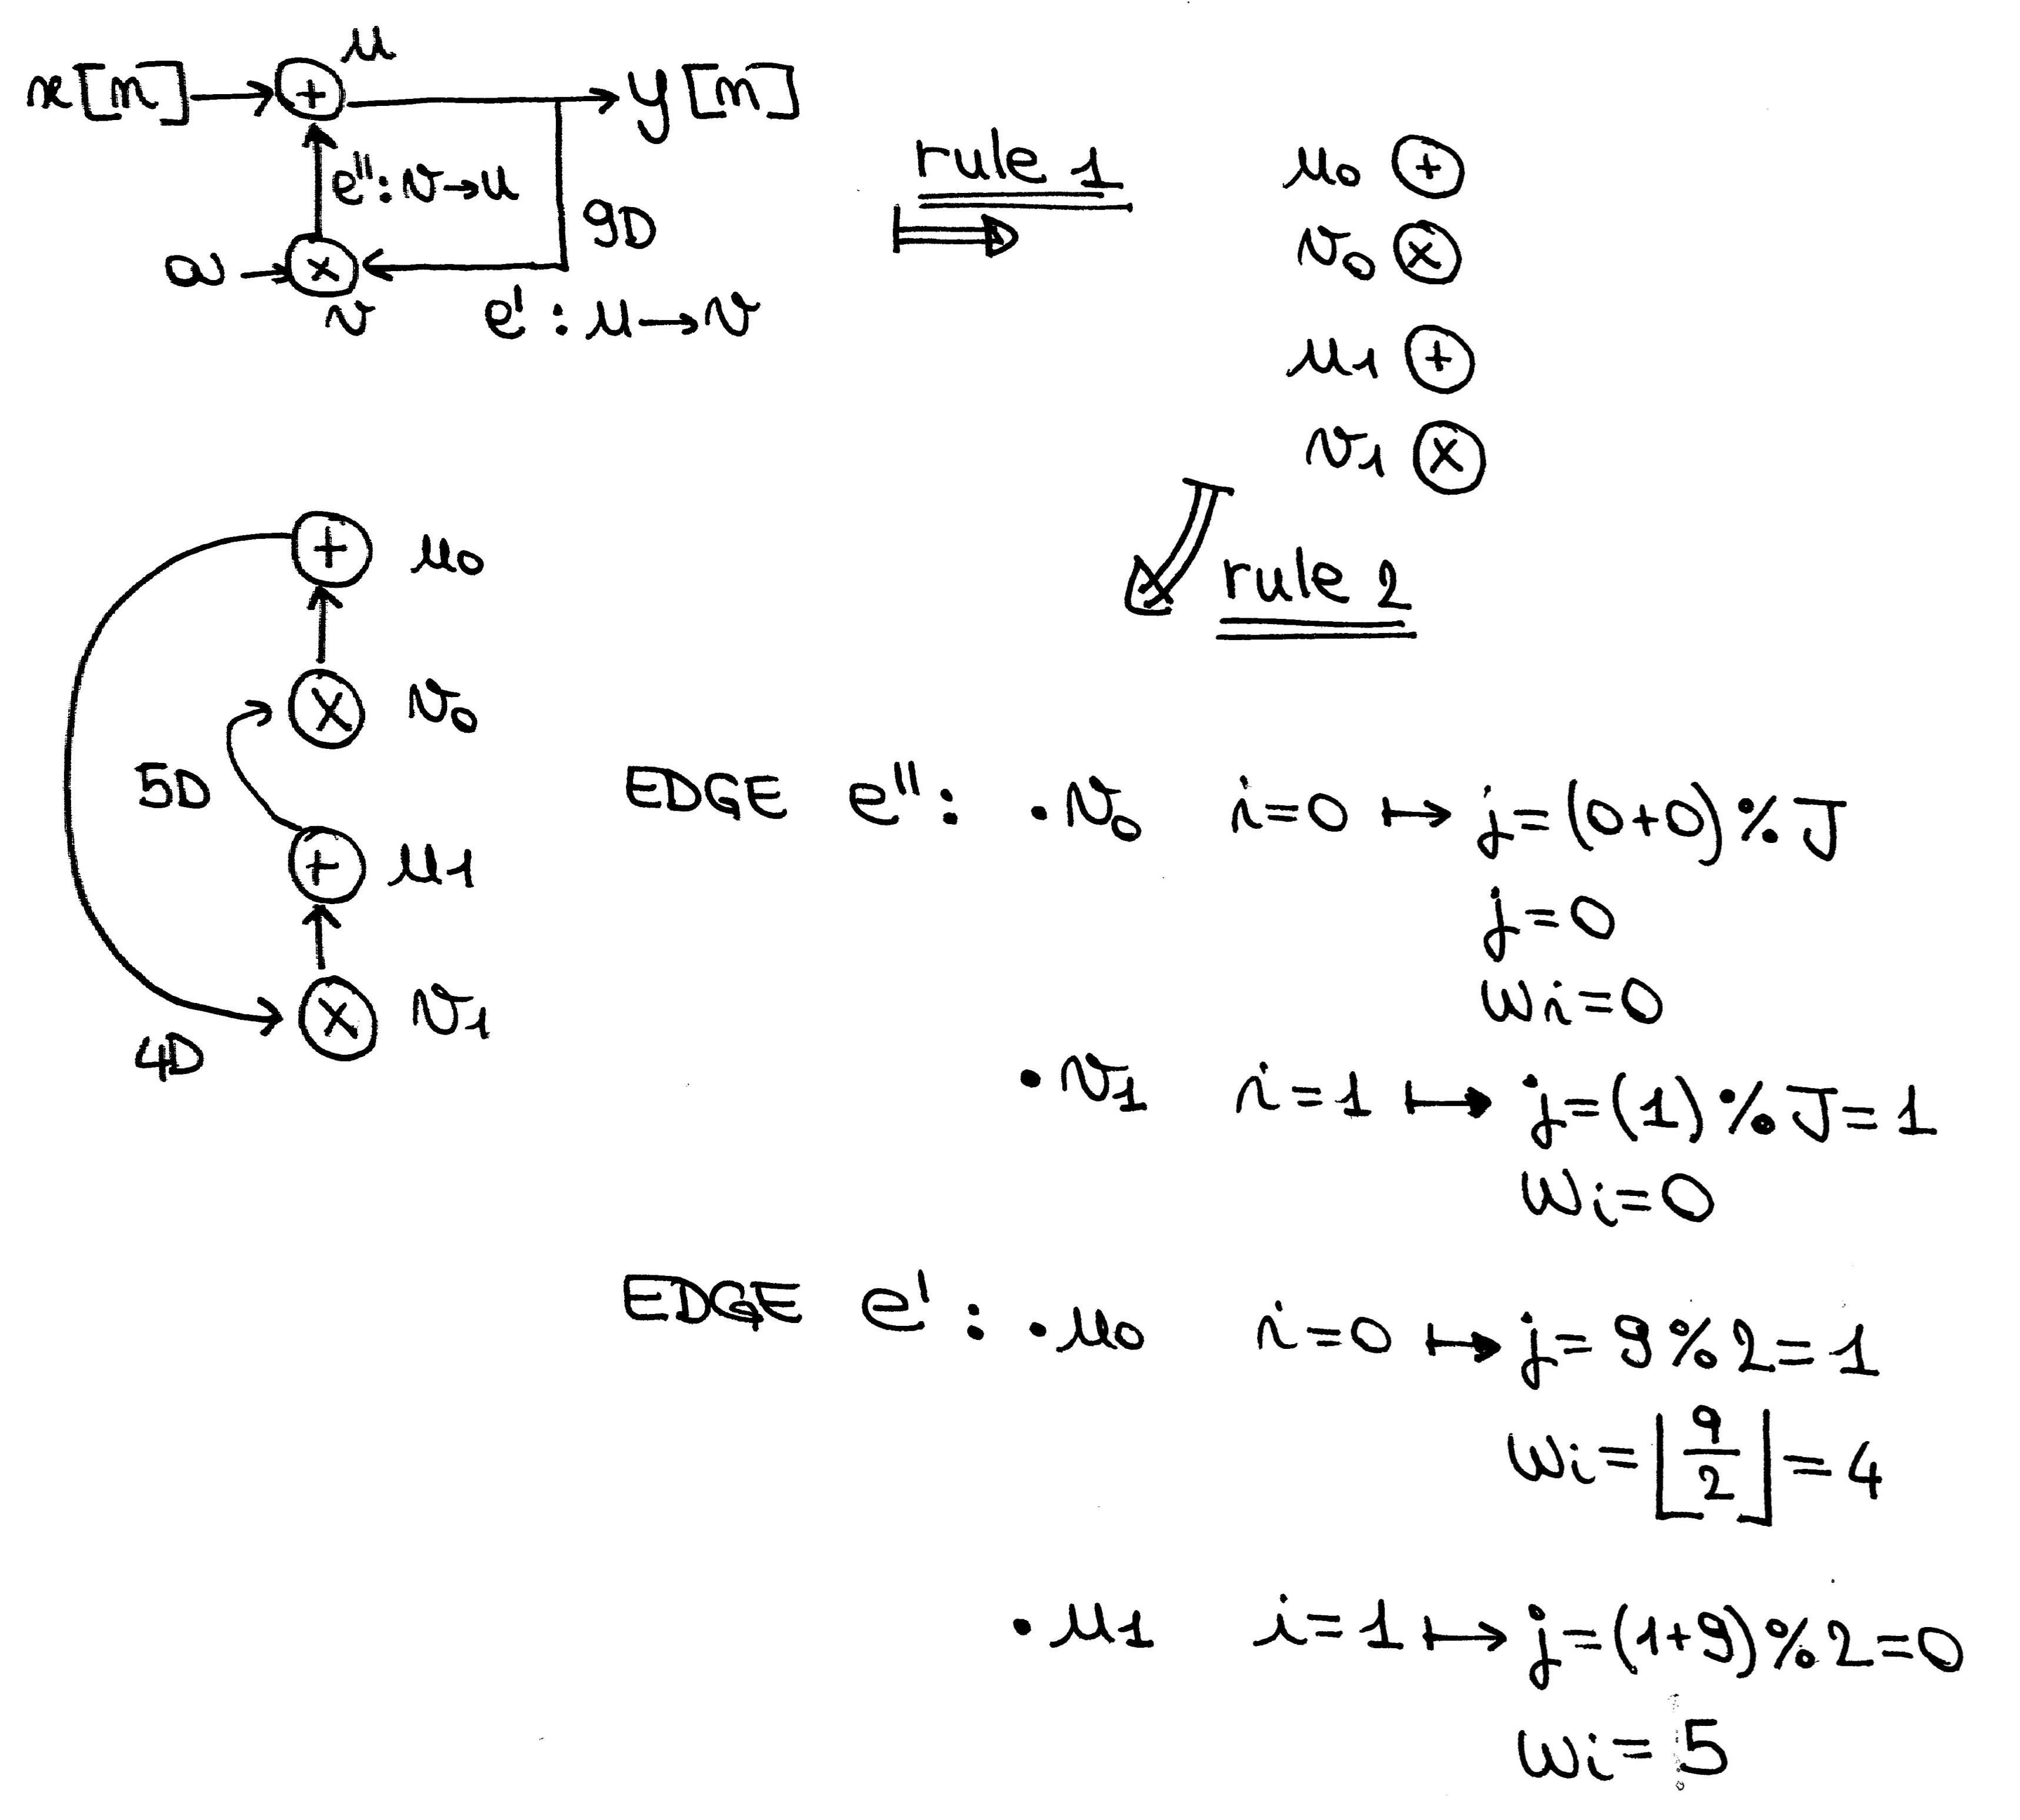
\includegraphics[width=0.7\linewidth]{img/img1/25}
\end{center}

We obtain exactly the same DFG as before.

\subparagraph{Example 2}

\begin{center}
  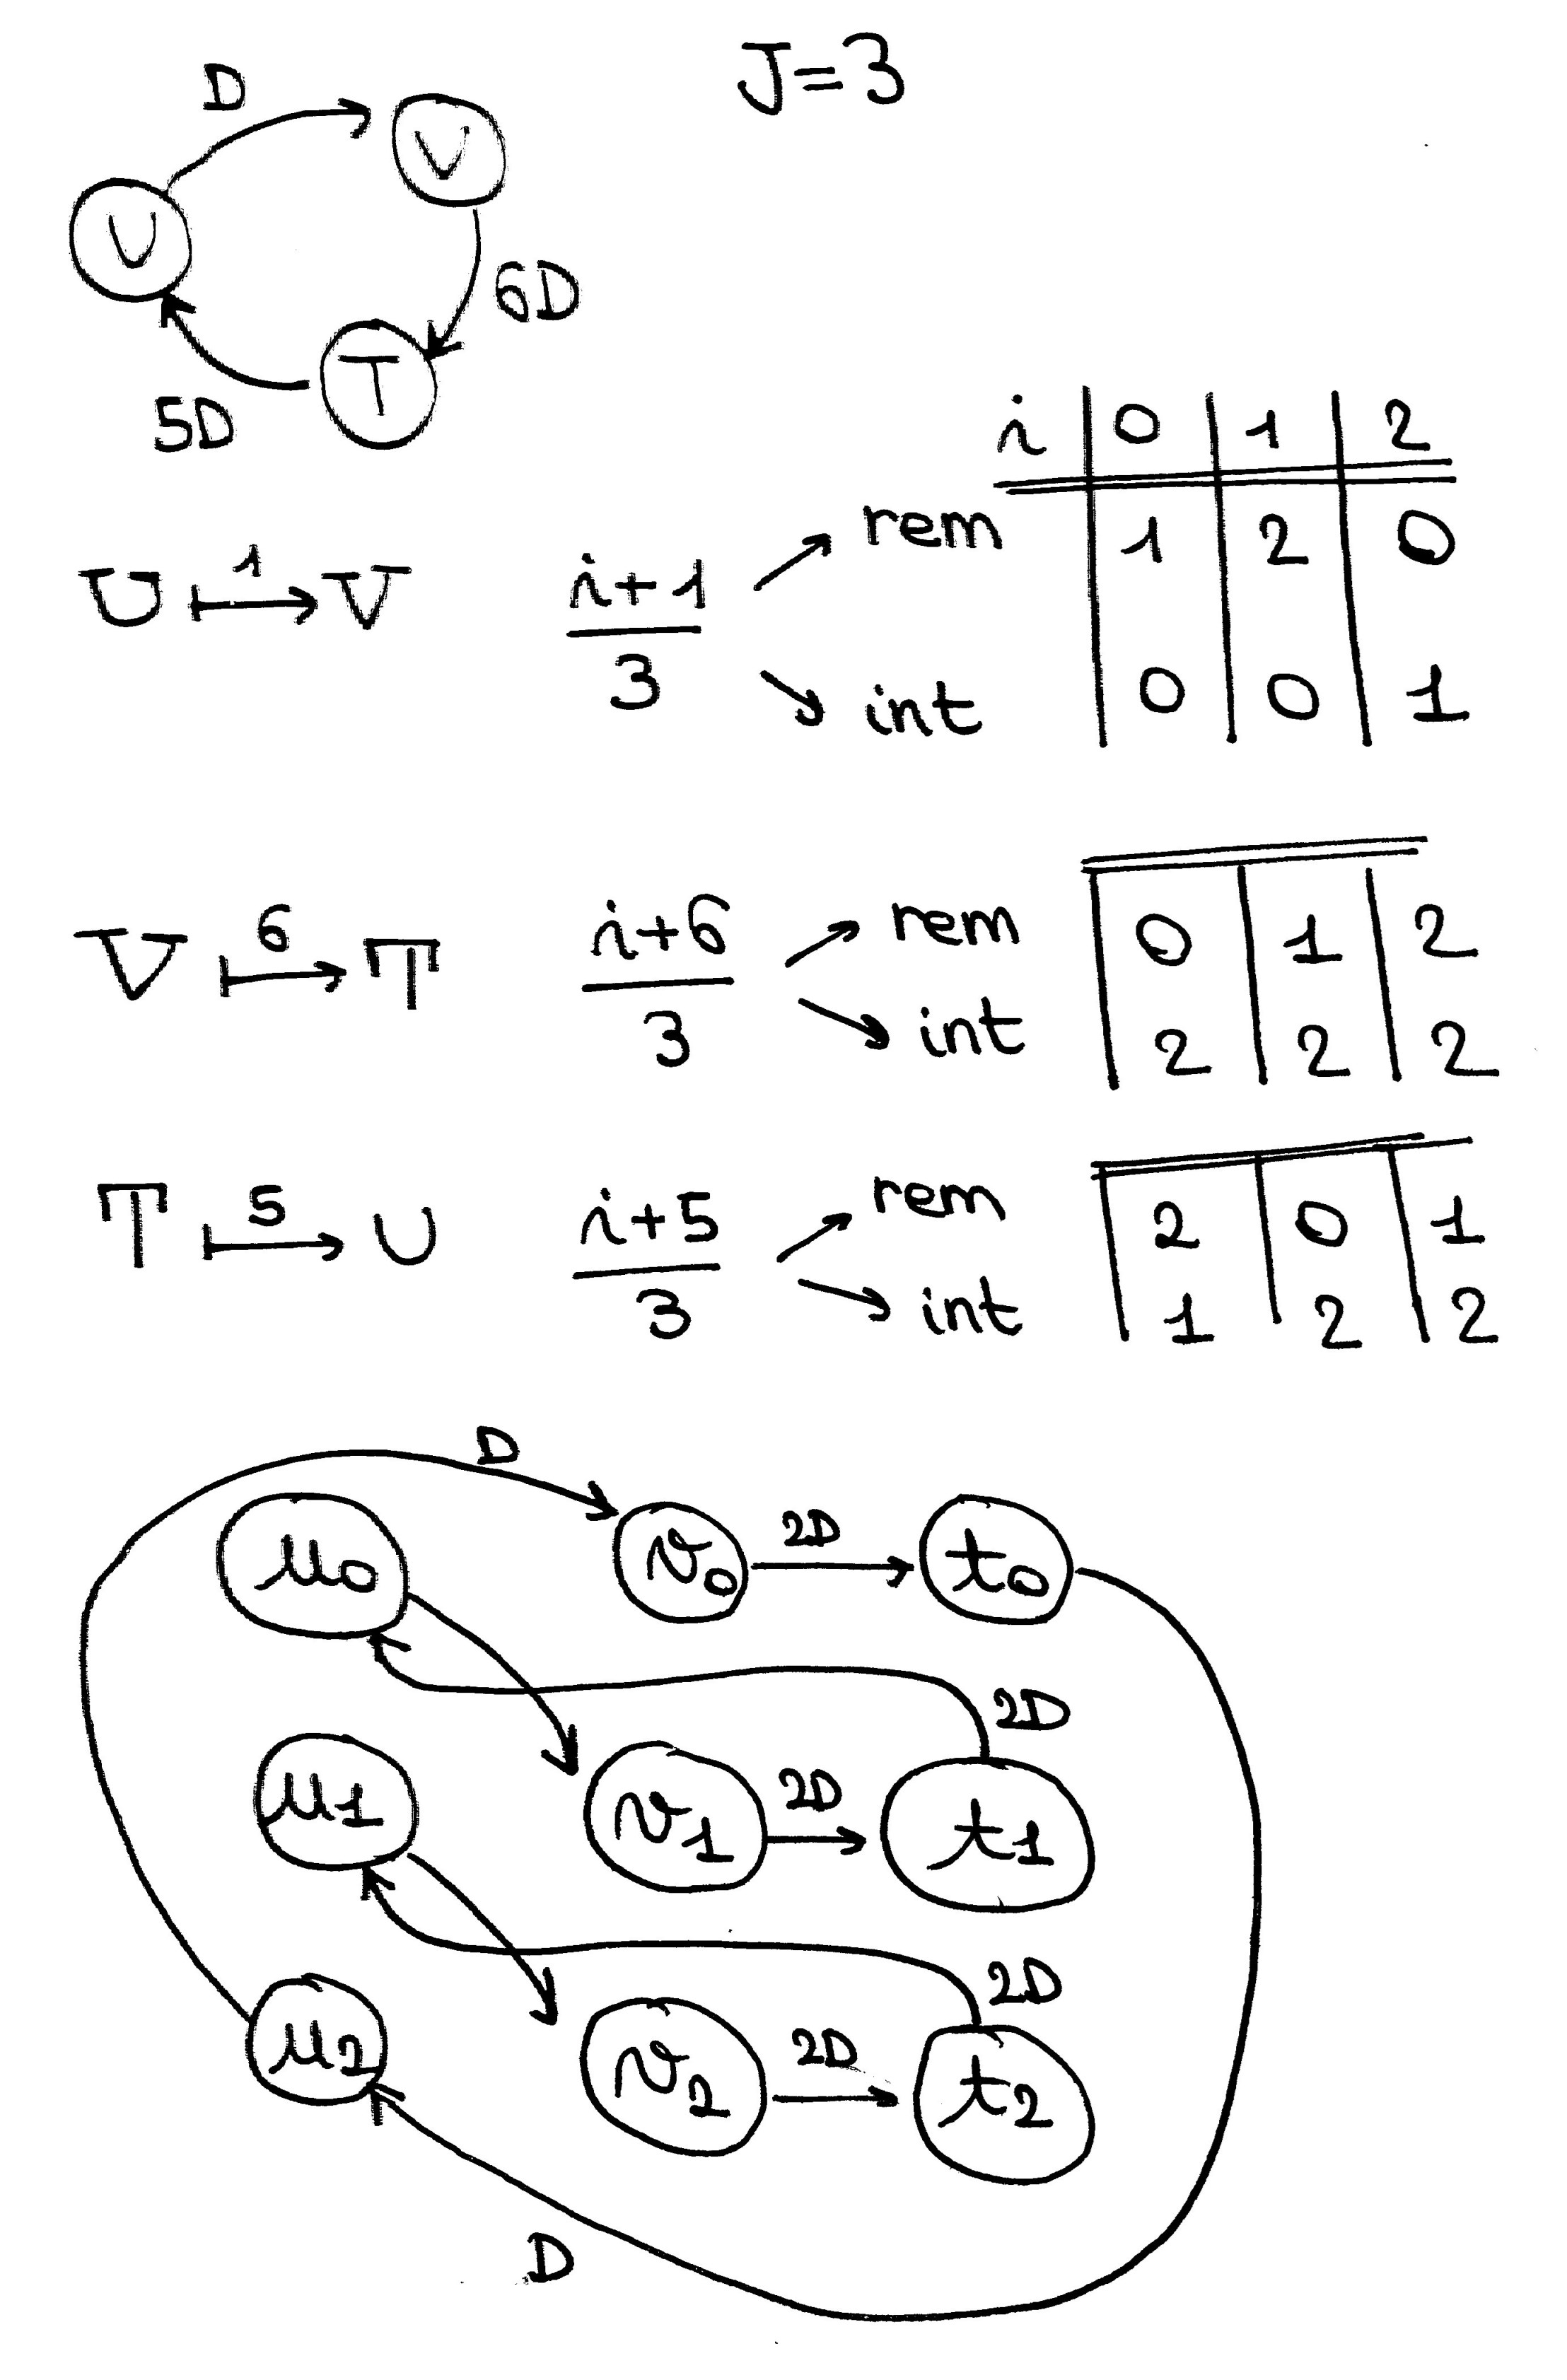
\includegraphics[width=0.7\linewidth]{img/img1/26}
\end{center}

Regarding speed up, implementing the original DFG (assuming all node v,u,t having same unit delay):
\begin{equation}
  T_{cp}=1  \hspace{10pt} th=1 \hspace{10 pt}  T_{\infty}=\frac{3}{12}=\frac{1}{4} < T_{cp}
\end{equation}
So we have the possibility to increase the throughput. Since retiming has no effect (because critical path is just across one node), we can apply a 3-degree unfolding, resulting in:
\begin{equation}
T_{cp}=2  \hspace{10pt} th=\frac{3}{2}=1.5
\end{equation}
So the critical path increases (this is quite common when applying unfolding) and the new throughput is not just the old one multiplies J but it is a little bit less. However now we can apply retiming to the new DFG (there are 2D between $T\rightarrow U$ which can be splitted one before and one after U), so:
\begin{equation}
T_{cp}=1  \hspace{10pt} th=3
\end{equation}

\subparagraph{Example fir filter}

\begin{center}
  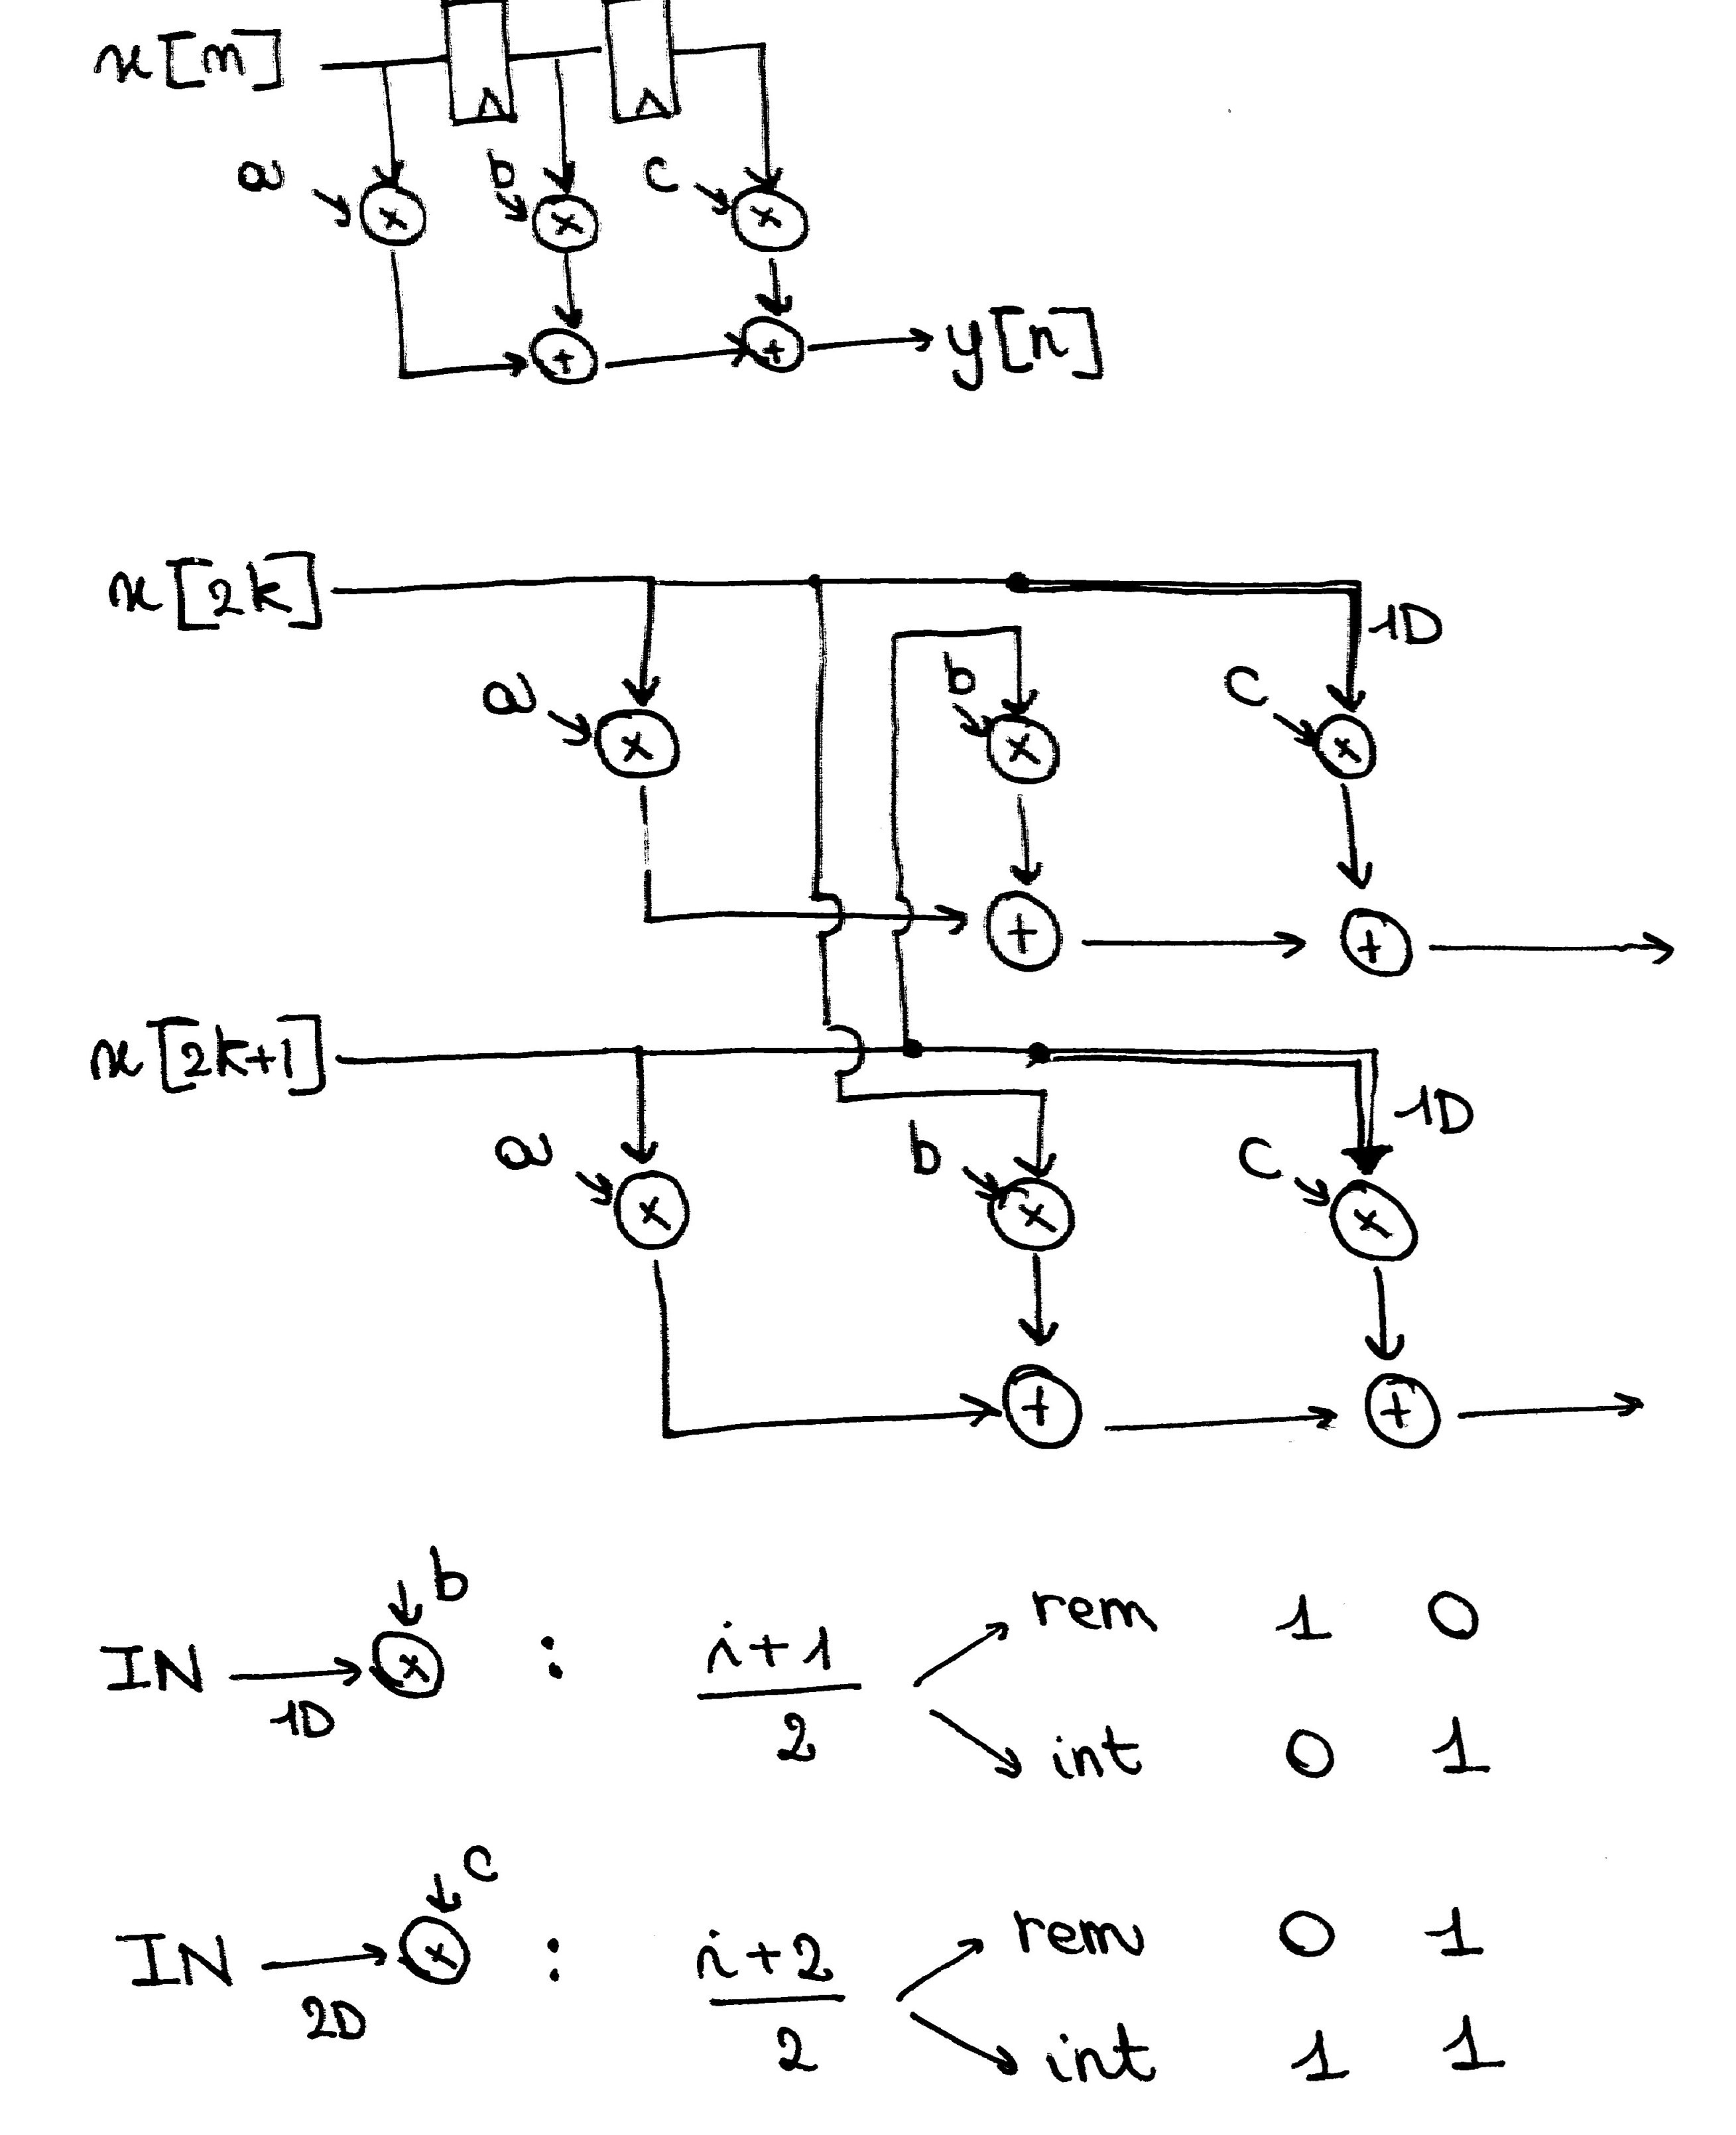
\includegraphics[width=0.9\linewidth]{img/img1/27}
\end{center}

In this particular case we can apply pipelining or unfolding (actually there are no loops but this technique can be applied to increase parallelism). Setting $J=2$ and noticing that for edges having $w=0$, it means that $j=i \% J= i$, as in the original DFG, therefore $w_i=\lfloor \frac{i}{J} \rfloor=0$, so no registers have to be added.\\

\textbf{Issue}: we can merge two registers together, so the number of registers doesn't change from the original one, meaning that applying unfolding the same amount of registers should be present in the original and unfolded DFG, provided some optimizations.


---- 17.10.2016
\section{Folding}
forse mancano i primi minuti...


Applying folding, we switch between two inputs:
\begin{center}
  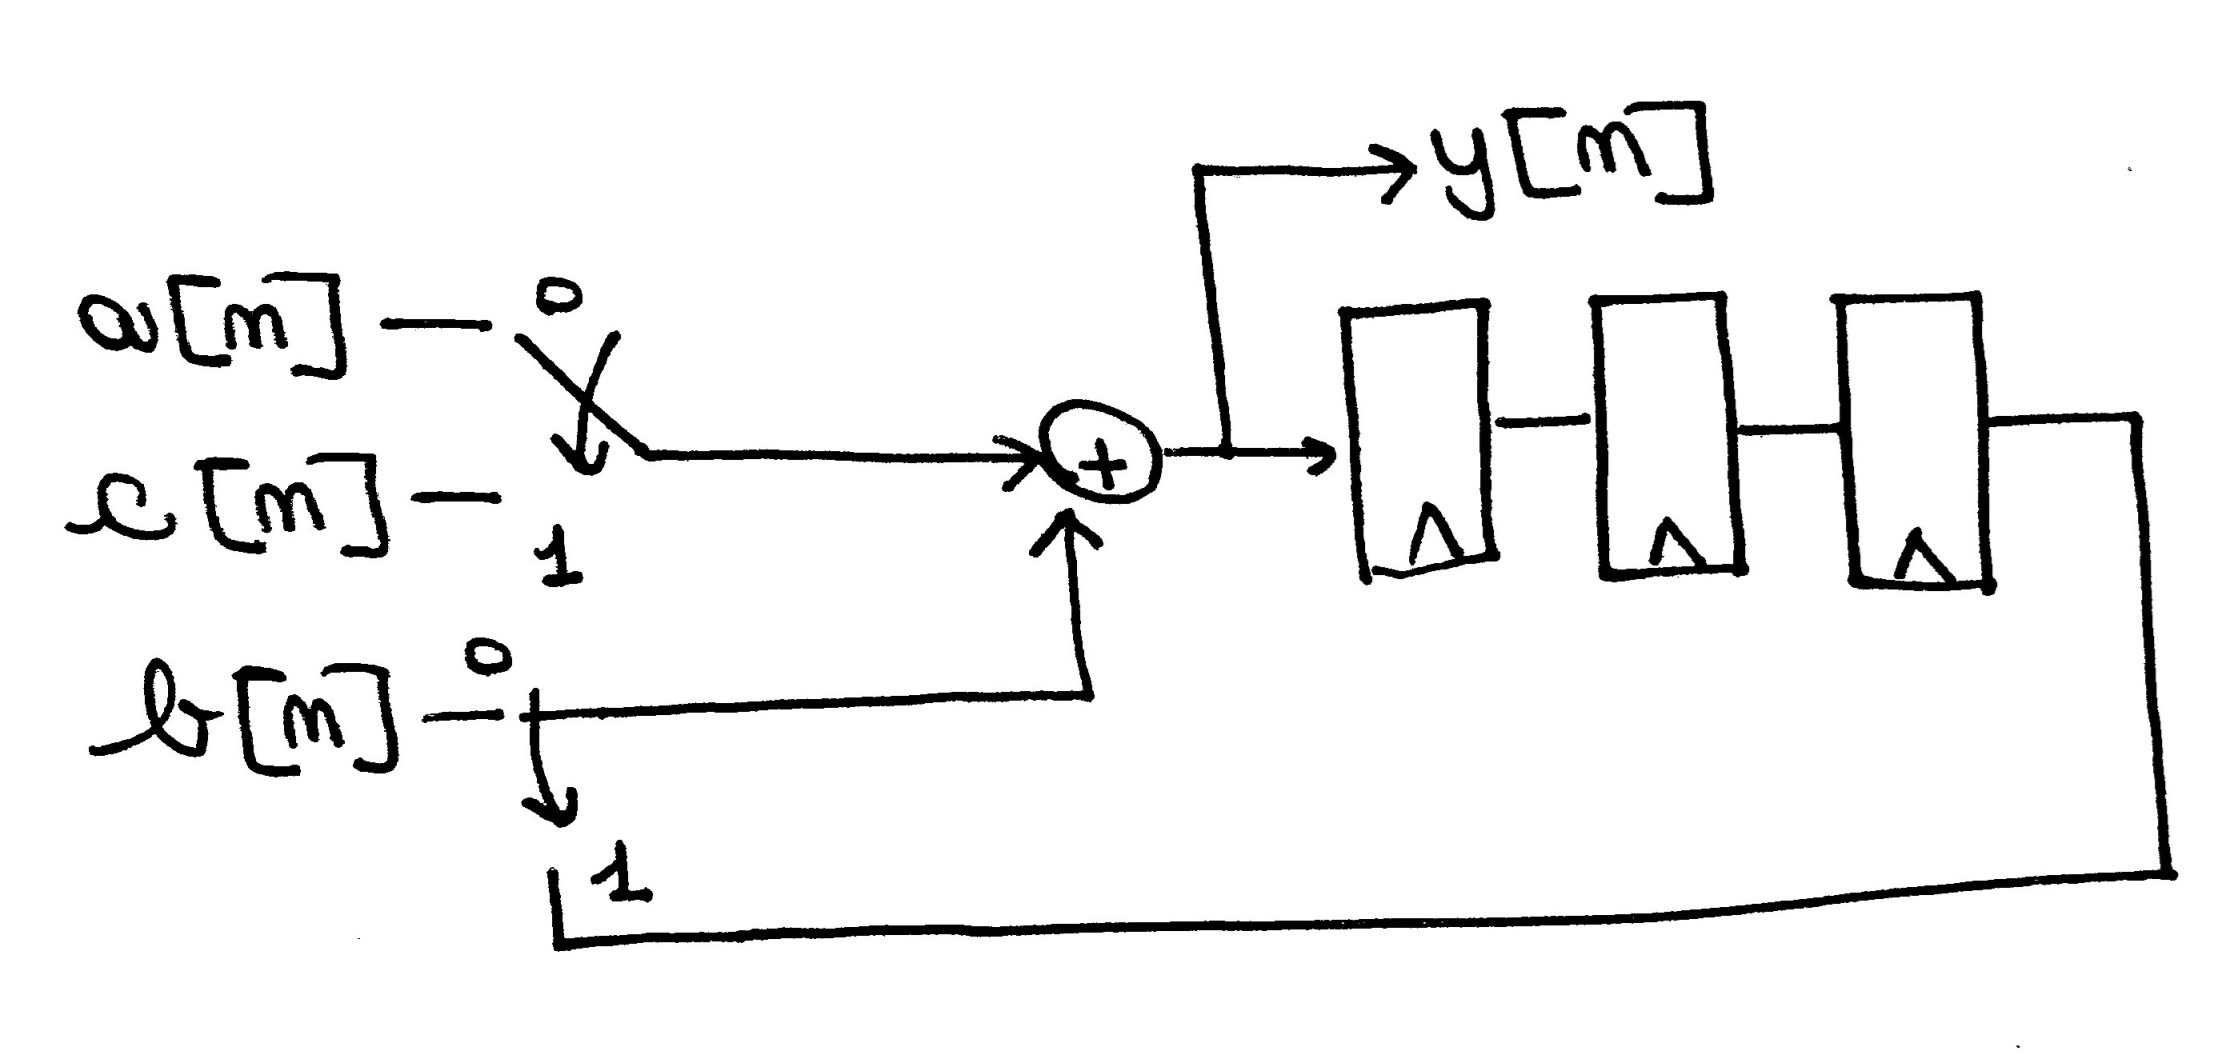
\includegraphics[width=0.6\linewidth]{img/img1/30}
\end{center}
In order to understand how many registers we need, we look at the same graph as before:
\begin{center}
  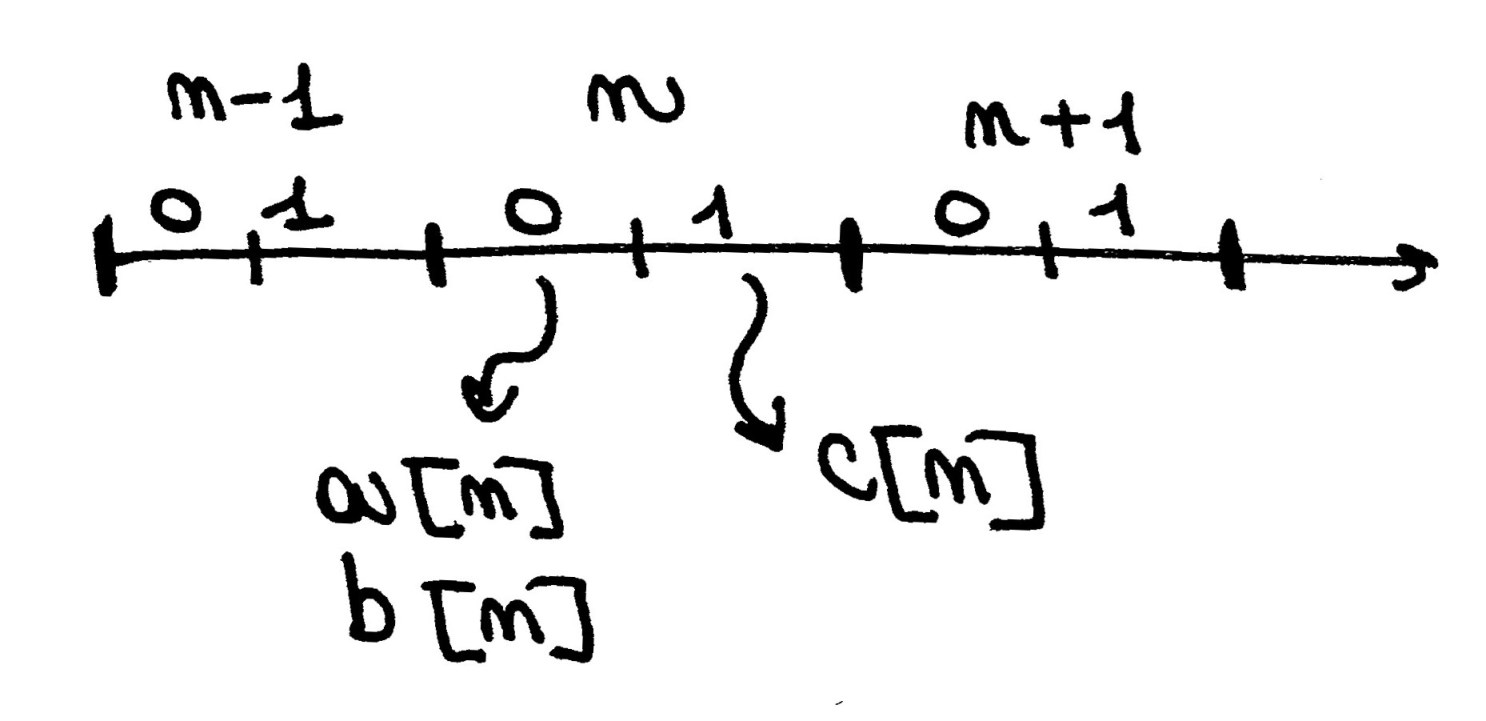
\includegraphics[width=0.6\linewidth]{img/img1/31}
\end{center}

At time index $n$ we receive $a[n]$ and $b[n]$, in the following clock cycle we receive $c[n]$ and since we cannot perform immediately the sum we need to insert three registers so we can delay $a[n-1]+b[n-1]$ to receive the third contribution $c[n]$.\\

In order to reuse hardware for different operations (such as the adder in the previous example), it's needed to properly evaluate the delay in order to insert the correct number of registers. In general we can proceed in the following way:

\begin{center}
  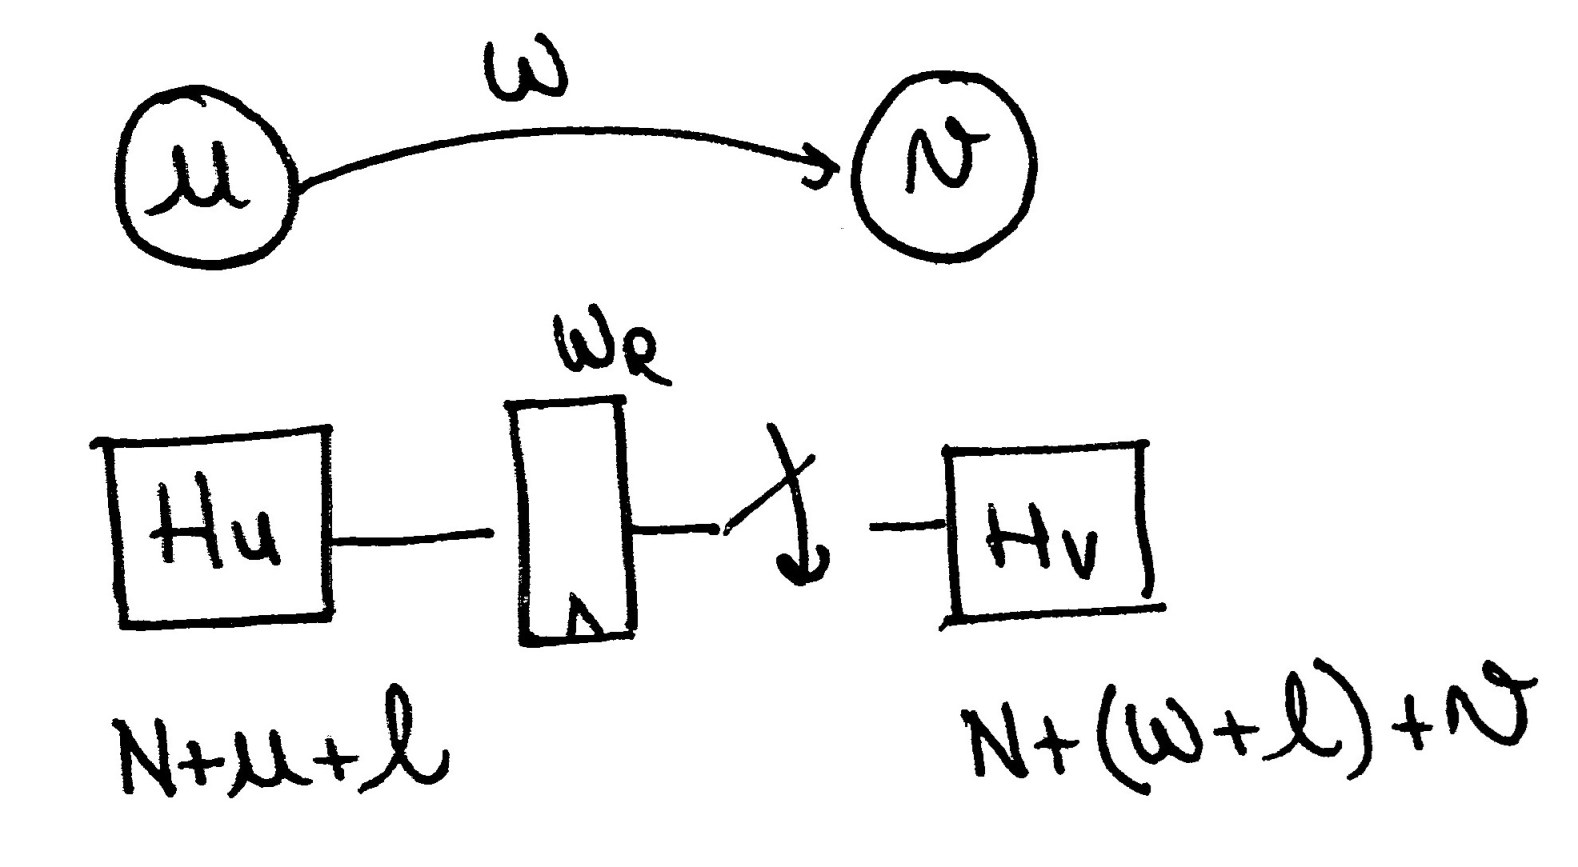
\includegraphics[width=0.6\linewidth]{img/img1/32}
\end{center}
Calling $u$ and $v$ two different operations (i.e. a certain sum in our algorithm), we need a certain type of hardware component in order to execute the operations, and this hardware block will be reuse in different steps. So we allocate hardware block $H_u$ and $H_v$ (i.e. adder, multiplier) that will be employed in different operation:
$$u \longrightarrow H_u$$
$$v \longrightarrow H_v$$

Calling $N$ the number of operations to be performed by a certain block hardware, the sample interval has to been divided in at least $N$ clock cycle. After that we have to \textbf{schedule the operations}, that means decide at which clock cycle execute a particular operation $u$:

scheduling time: u for U executed by $H_u$
v for V executed by $H_v$

In the final DFG we will have block $H_u$ and  $H_v$ , then the output of a certain operation $u$ will be available at the output of $H_u$ at time $N+l+u$. In the same way at the input of $H_v$ TODO NON CHIARO N+(l+w)+v, meaning that $u$ and $v$ determine the scheduling of operation in $N$, $l$ is an integer value, $w$ is the number of register in the original DFG. At the end we have to place between $H_u$ and $H_v$ a number of registers equal to:
$w_f=N+w+v-u$

\subparagraph{Example with FIR filter}

\begin{center}
  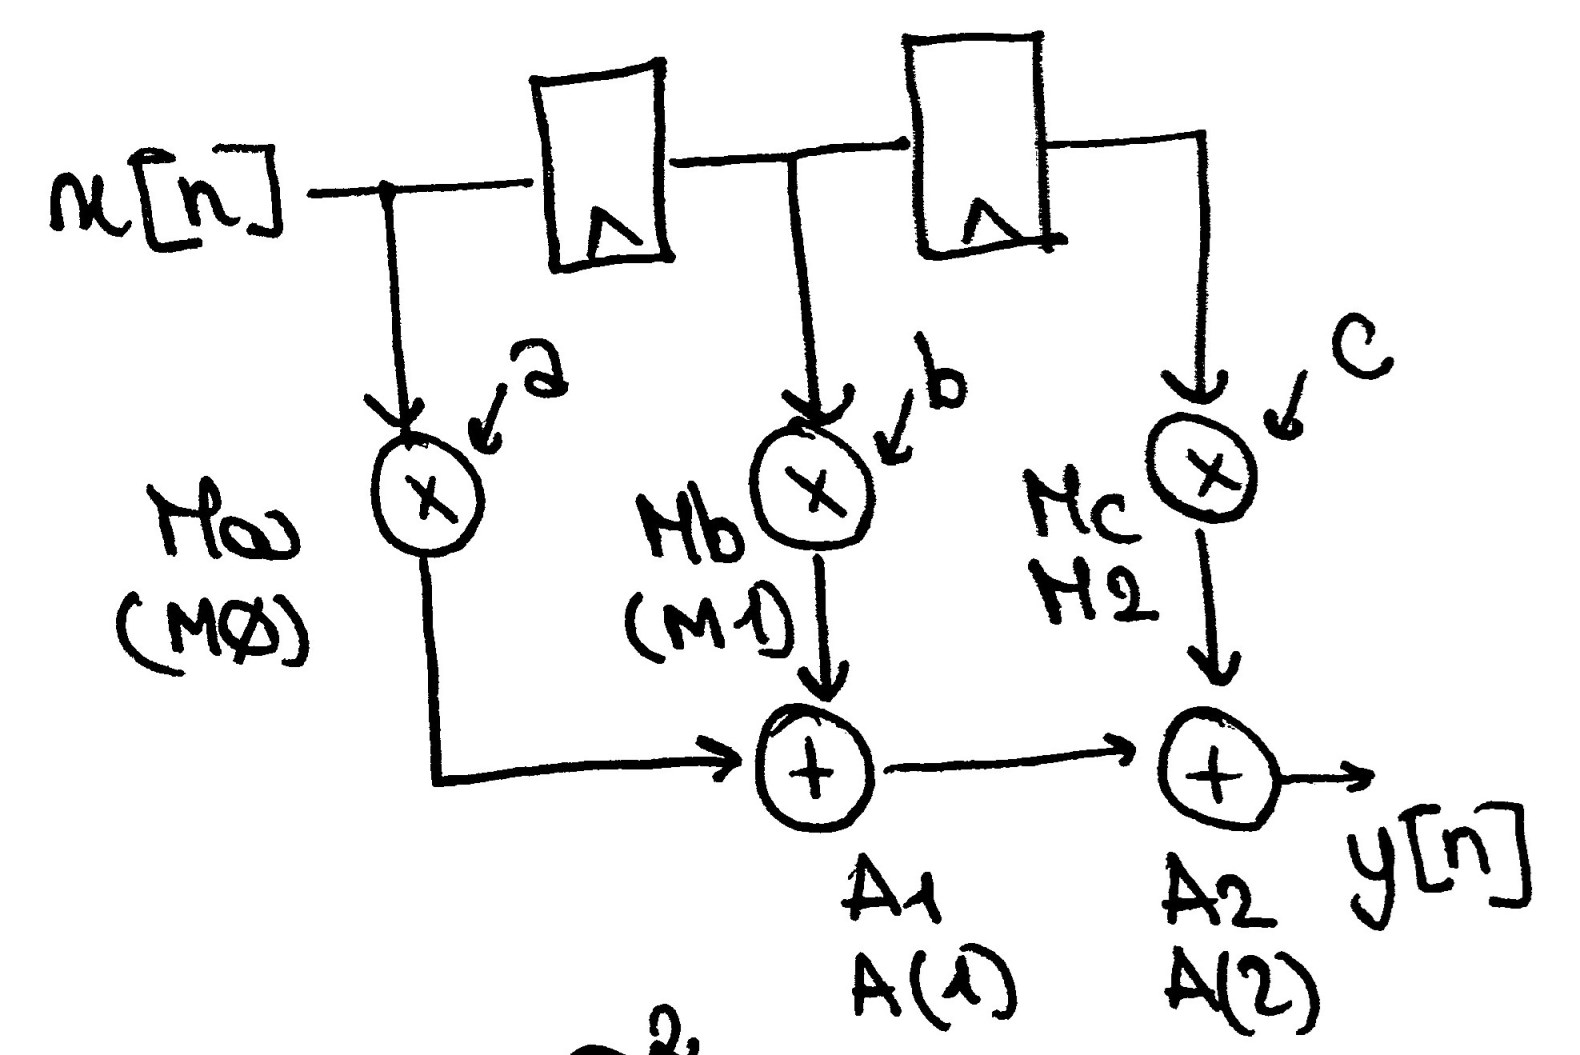
\includegraphics[width=0.6\linewidth]{img/img1/33}
\end{center}

We have to perform two addition and three multiplications using one adder and one multiplier. In this case we select $N=3$.

Scheduling for multiplication:
\begin{verbatim}
in c.c =0  -> multiplier: multiplication *a
in c.c =1  -> multiplier: multiplication *b
in c.c =2  -> multiplier: multiplication *c
\end{verbatim}

Scheduling for sum (multiple choices):
\begin{verbatim}
in c.c =0  -> none
in c.c =1  -> adder: (+b*..)  (A_1)
in c.c =2  -> adder: (+c*..)  (A_2)
\end{verbatim}

The new DFG becomes:

\begin{center}
  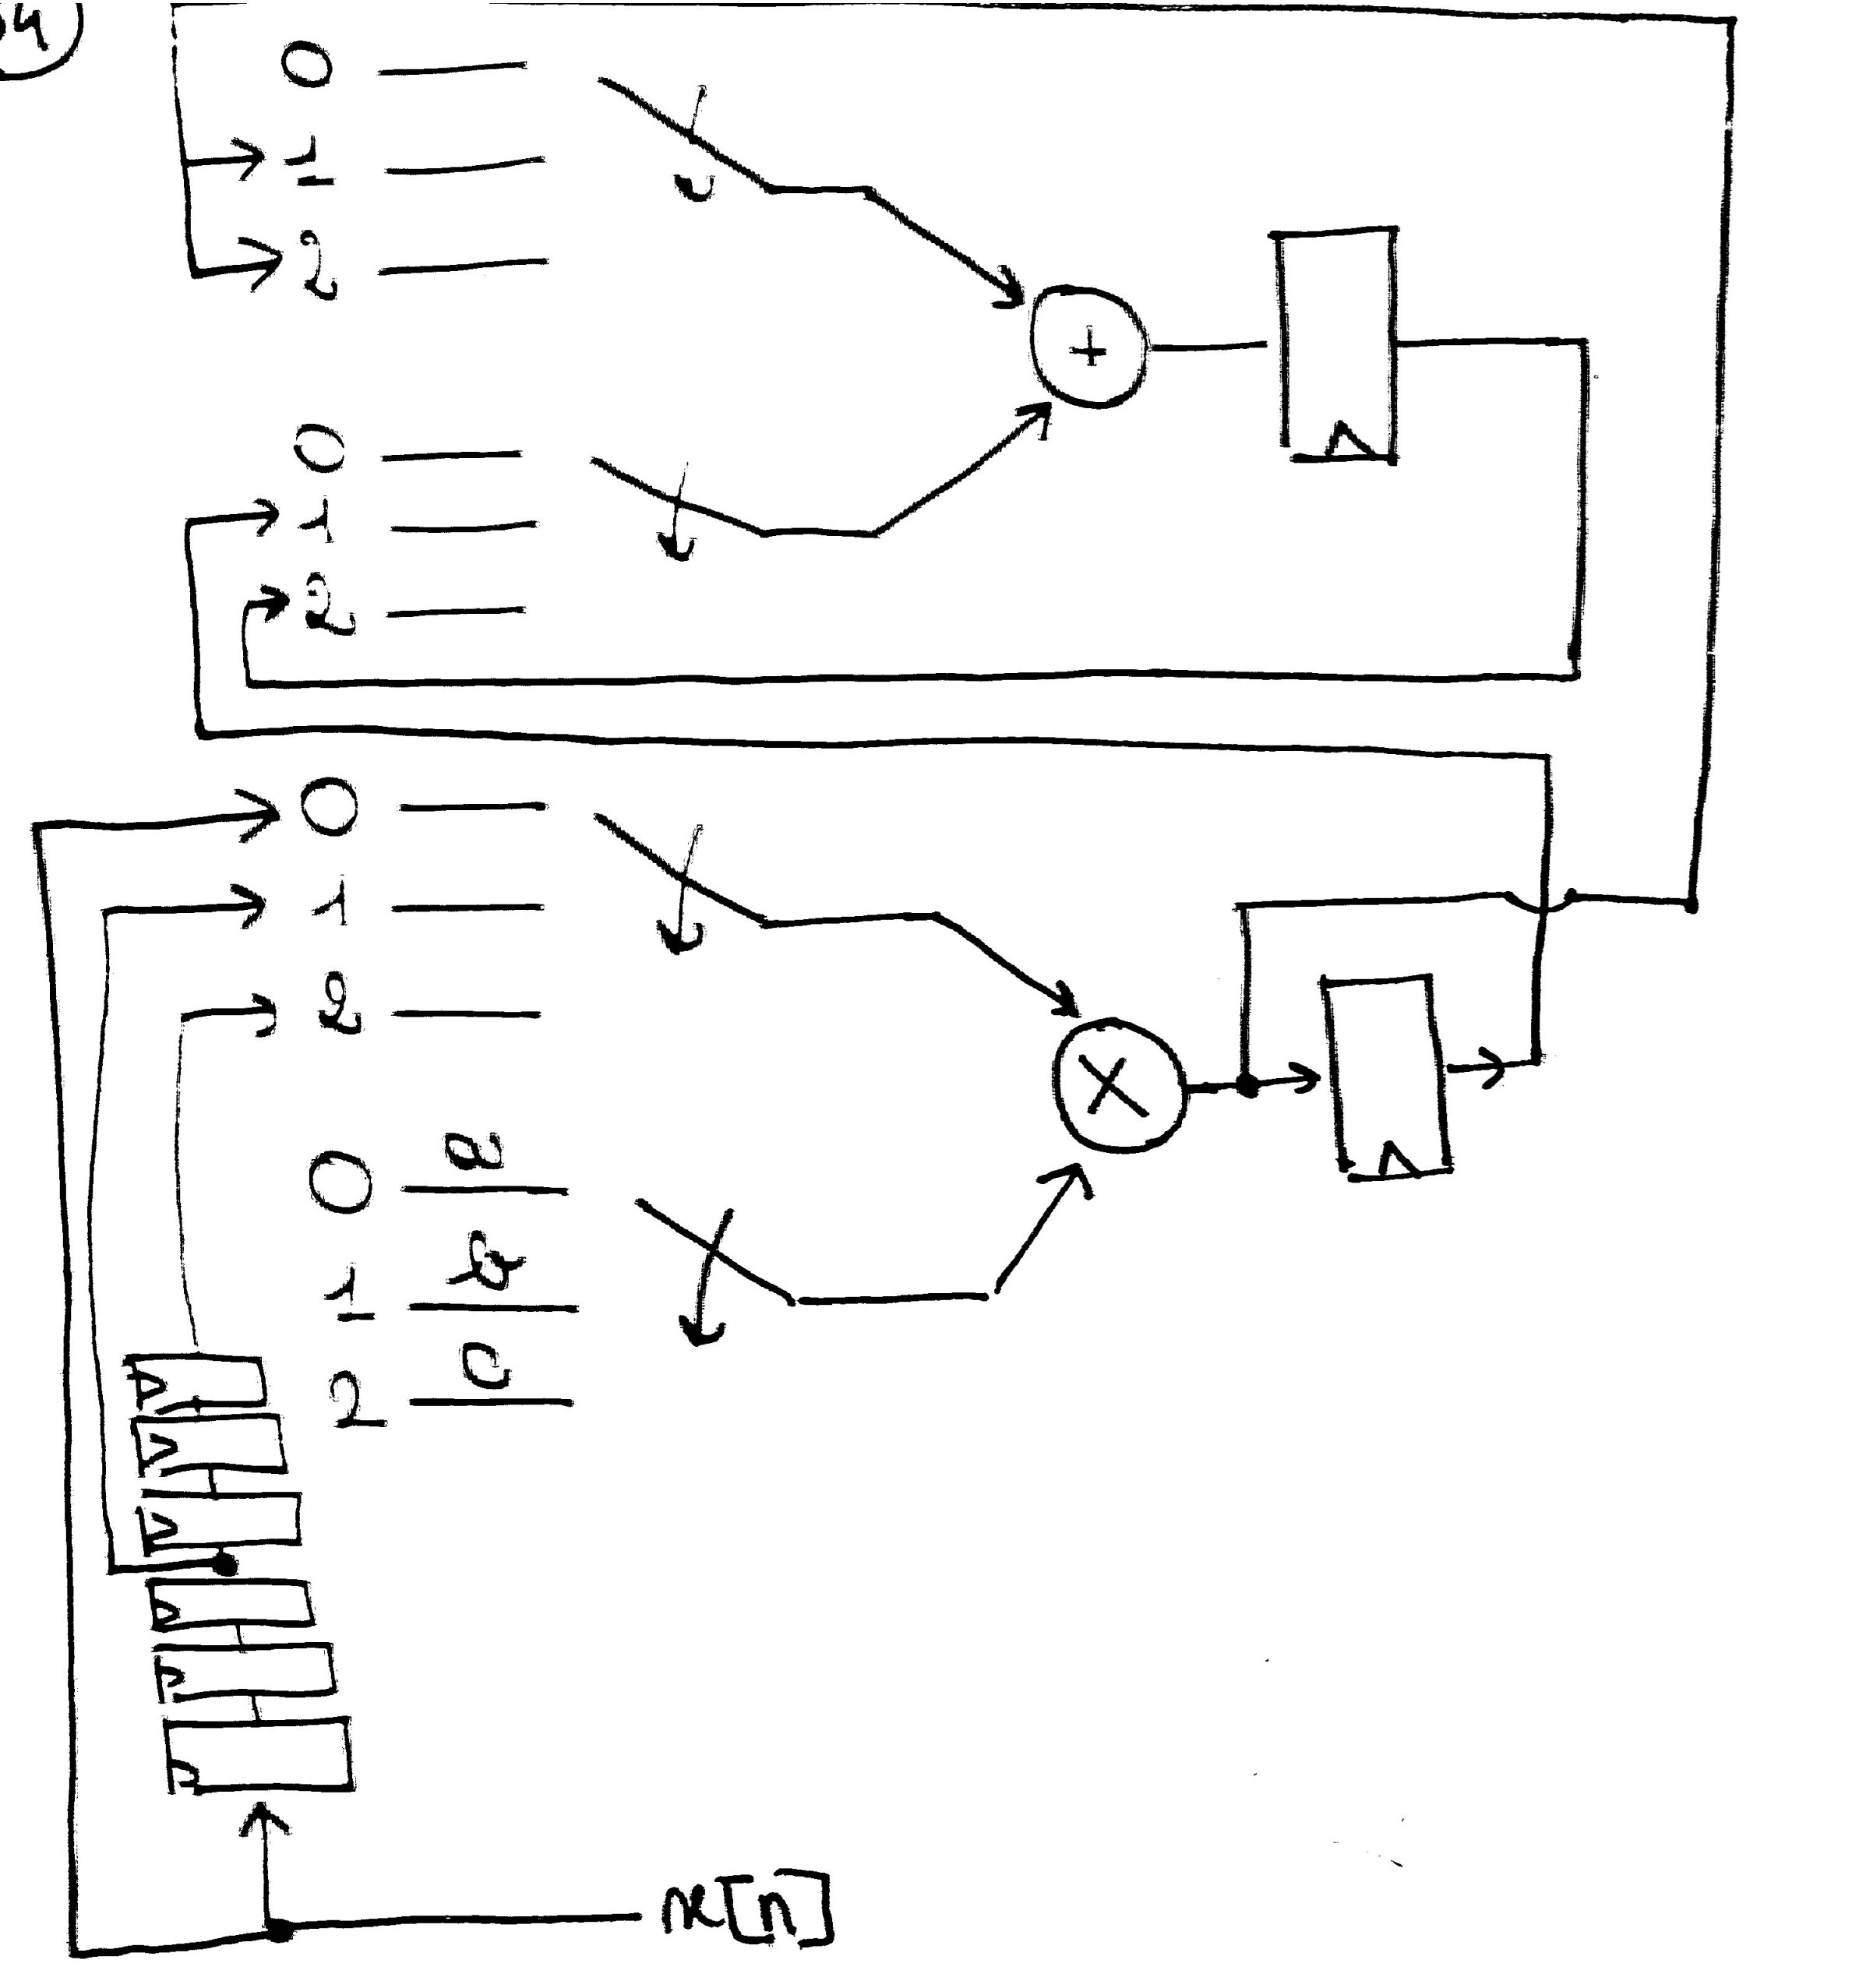
\includegraphics[width=0.7\linewidth]{img/img1/34}
\end{center}

For every connection between the adder ant the multiplier, we need to derive the proper number of registers to be inserted:
\begin{center}
  \begin{tabular}{|l|c|c|c|c|}
  \hline
  Edge &                $w$&    $u$ (source node)&    $v$ (dest node)&    $w_f=N+w+v-u$\\
  \hline
  $M_a \longrightarrow A_1$&      0&      0&            1&            1\\
  $M_b \longrightarrow A_1$&      0&      1&            1&            0 \\
  $M_c \longrightarrow A_2$&      0&      2&            2&            0 \\
  $A_1 \longrightarrow A_2$&      0&      1&            2&            1\\
  $IN \longrightarrow M_a$&     0&      0&            0&            0 \\
  $IN \longrightarrow M_b$&     1&      1?&           1&            3\\
  $IN \longrightarrow M_c$&     2&      2?&           2&            6\\
  \hline
  \end{tabular}
\end{center}

In clock cycle number 1 the adder receive on one side the multiplication executed in the same clock cycle and on the other side the output of the multiplier delayed by 1. In clock cycle 0  nothing has to been connected to the adder since it's not used.\\

We still have to understand how the input samples have to be applied to the multiplier, so we can apply the same methodology for the edge from $x[n]$ (virtual node IN) to the multiplier. Making some assumptions, we assume that the input data $x[n]$ is valid for three clock cycles (meaning that for 3 clock cycles there will be at the input $x[n]$ and for the next 3 clock cycles $x[n+1]$): for all the sampling interval data are stable. Therefore we can choose as $u$ for the last three operation a number that reduce the amount of required registers.\\

In this example there are three multiplications in 3 clock cycles, so the scheduling it's already fixed. Regarding sums, we could have choice a different scheduling ($A_1$ in c.c. 0 and $A_2$ in c.c. 1). However the starting DFG also gives us data dependencies: ignoring them results in $w_f < 0$ which is unphysical. To fix this problem, we need to change the scheduling time so that for each edge $w_f$ is always non negative: since this is a global problem, just fixing an edge we can affect the others and not resolve the problem. If we are not able to find a solution, we can change the original DFG using re-timing to have at least one register on the edge resulting in $w_f<0$. In this way we can respect data dependencies working in different sampling interval.

\subparagraph{example 2}

\begin{center}
  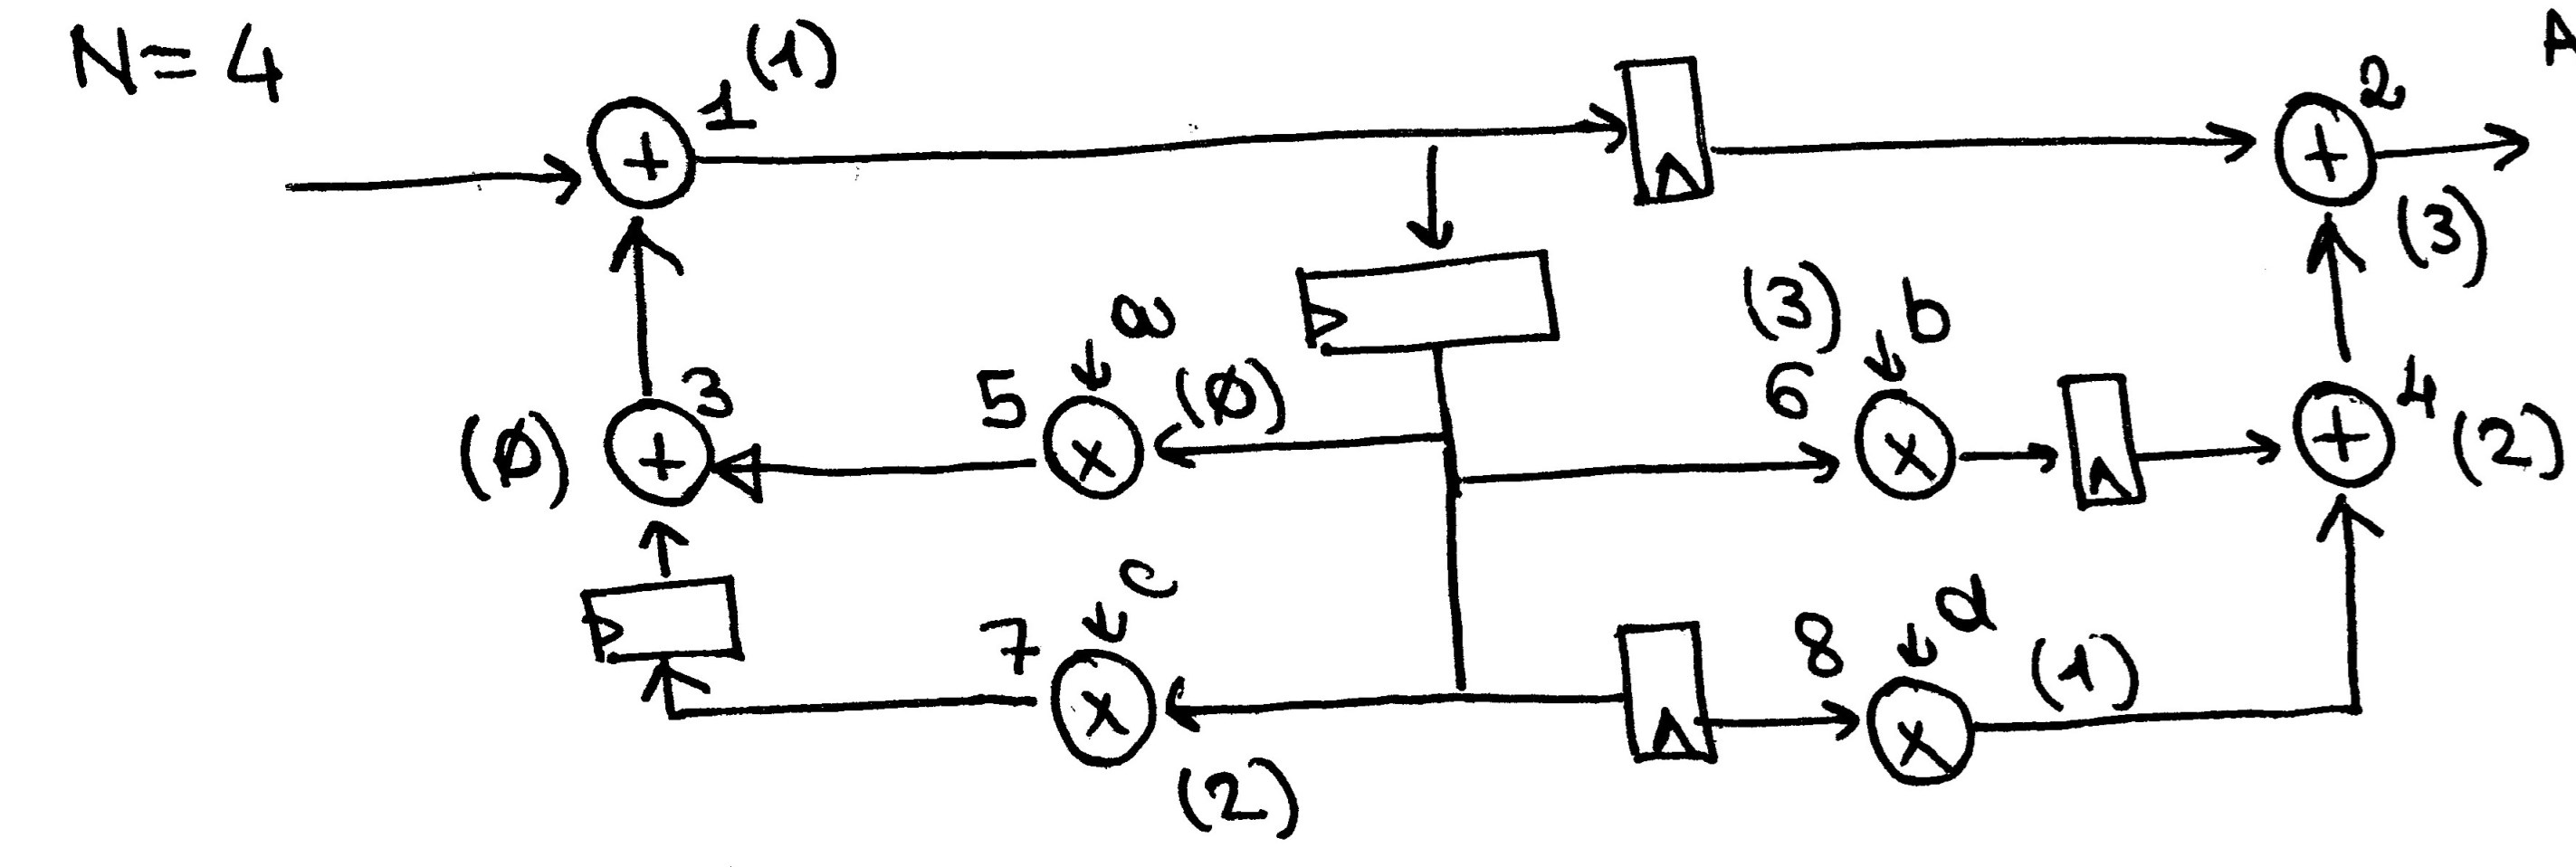
\includegraphics[width=0.7\linewidth]{img/img1/35}
\end{center}

Operations 1..4 represent 4 sums, 5..8 are 4 multiplications. Choosing as scheduling time the one in brackets:

Since $N=4$ it means that we have one adder and one multiplier. The criterion used for this assignment is that where there are no registers on one edge, it's convenient to use increasing index to respect data dependencies, instead where there is at least one register no problem regarding data dependencies will occur independently from the chosen scheduling.

\begin{center}
  \begin{tabular}{|c|c|c|c|c|c|}
    \hline
    Source &  Destination&  $w$ & $v$&  $u$&  $w_f=N+w+v-u$\\
    \hline
      1&      2&      1&    3&    1&    6\\
      1&      5&      1&    0&    1&    3\\
      1&      6&      1&    3&    1&    6\\
      1&      7&      1&    2&    1&    5\\
      1&      8&      2&    1&    1&    8\\
      \hline
      3&      1&      0&    1&    0&    1\\
      5&      3&      0&    0&    0&    0\\
      7&      3&      1&    0&    2&    2\\
      4&      2&      0&    3&    2&    1\\
      6&      4&      1&    2&    3&    3\\
      8&      4&      0&    2&    1&    1\\
    \hline
  \end{tabular}
\end{center}

So it's possible to map directly the architecture as in the previous cases, obtaining:

\begin{center}
  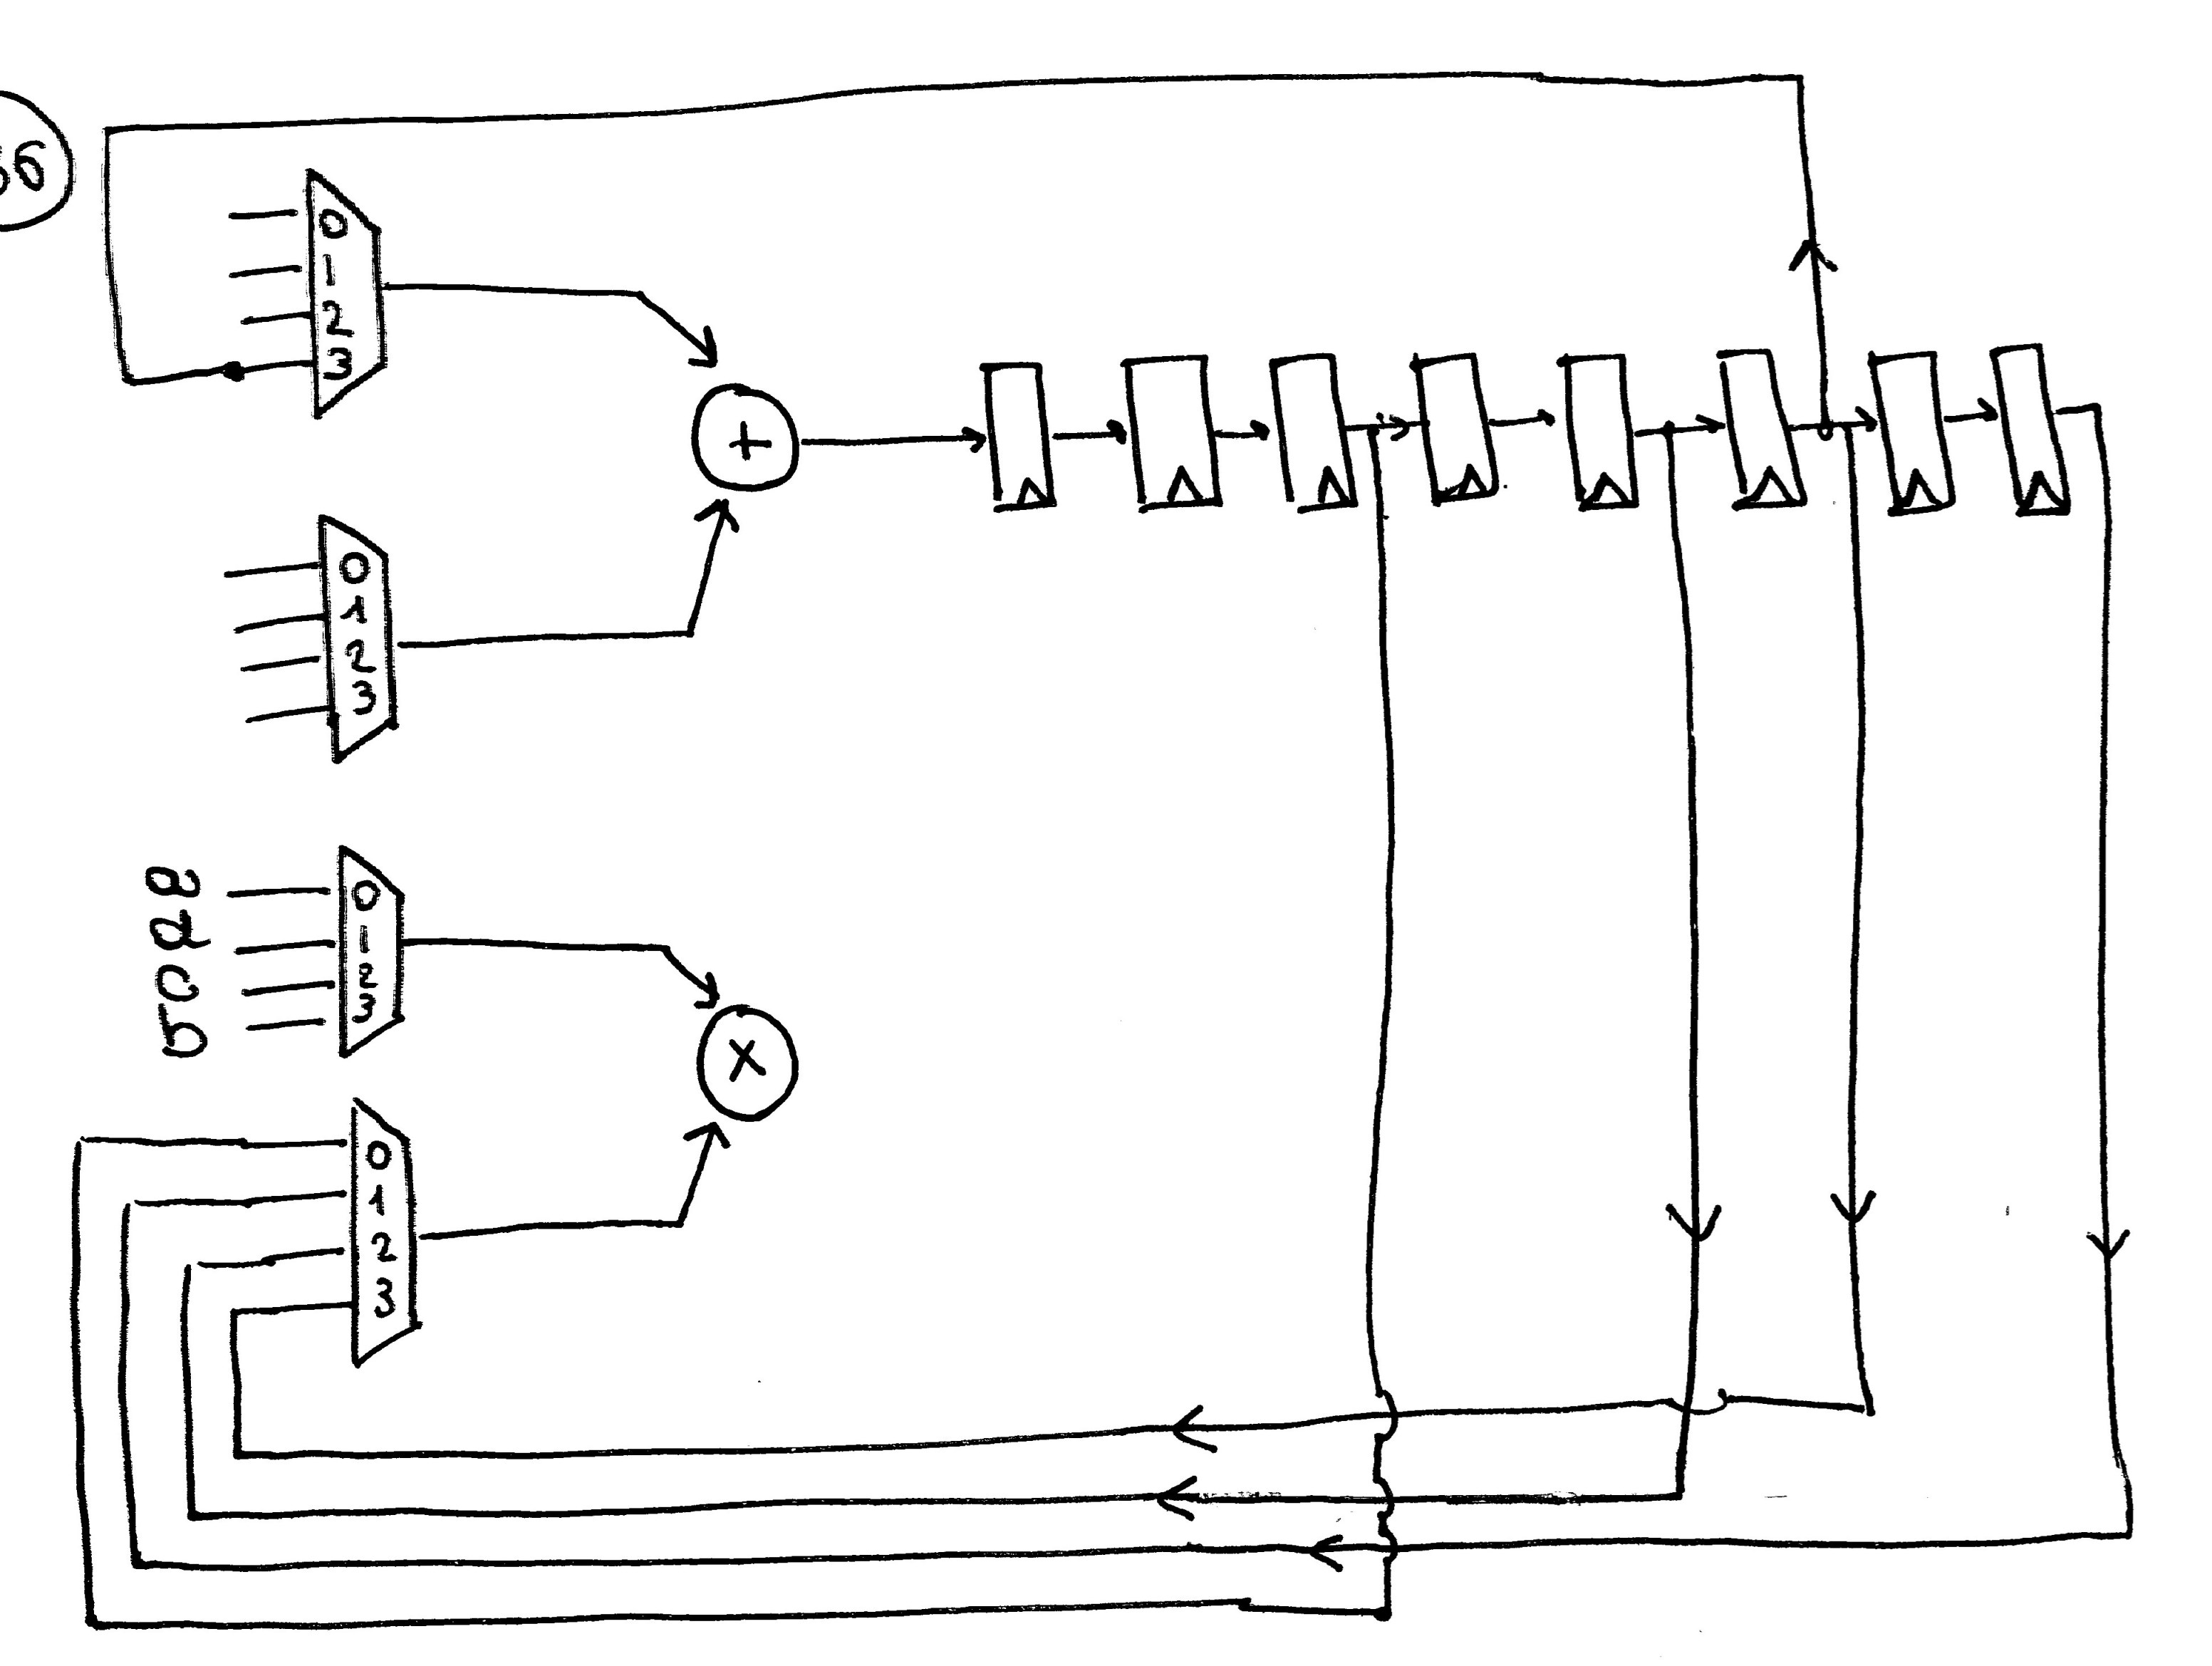
\includegraphics[width=0.7\linewidth]{img/img1/36}
\end{center}

At the input of multiplier we have coefficients and always the output of node 1 with a different delay.

\section{Decomposition}

\paragraph{Summary}
\begin{center}
  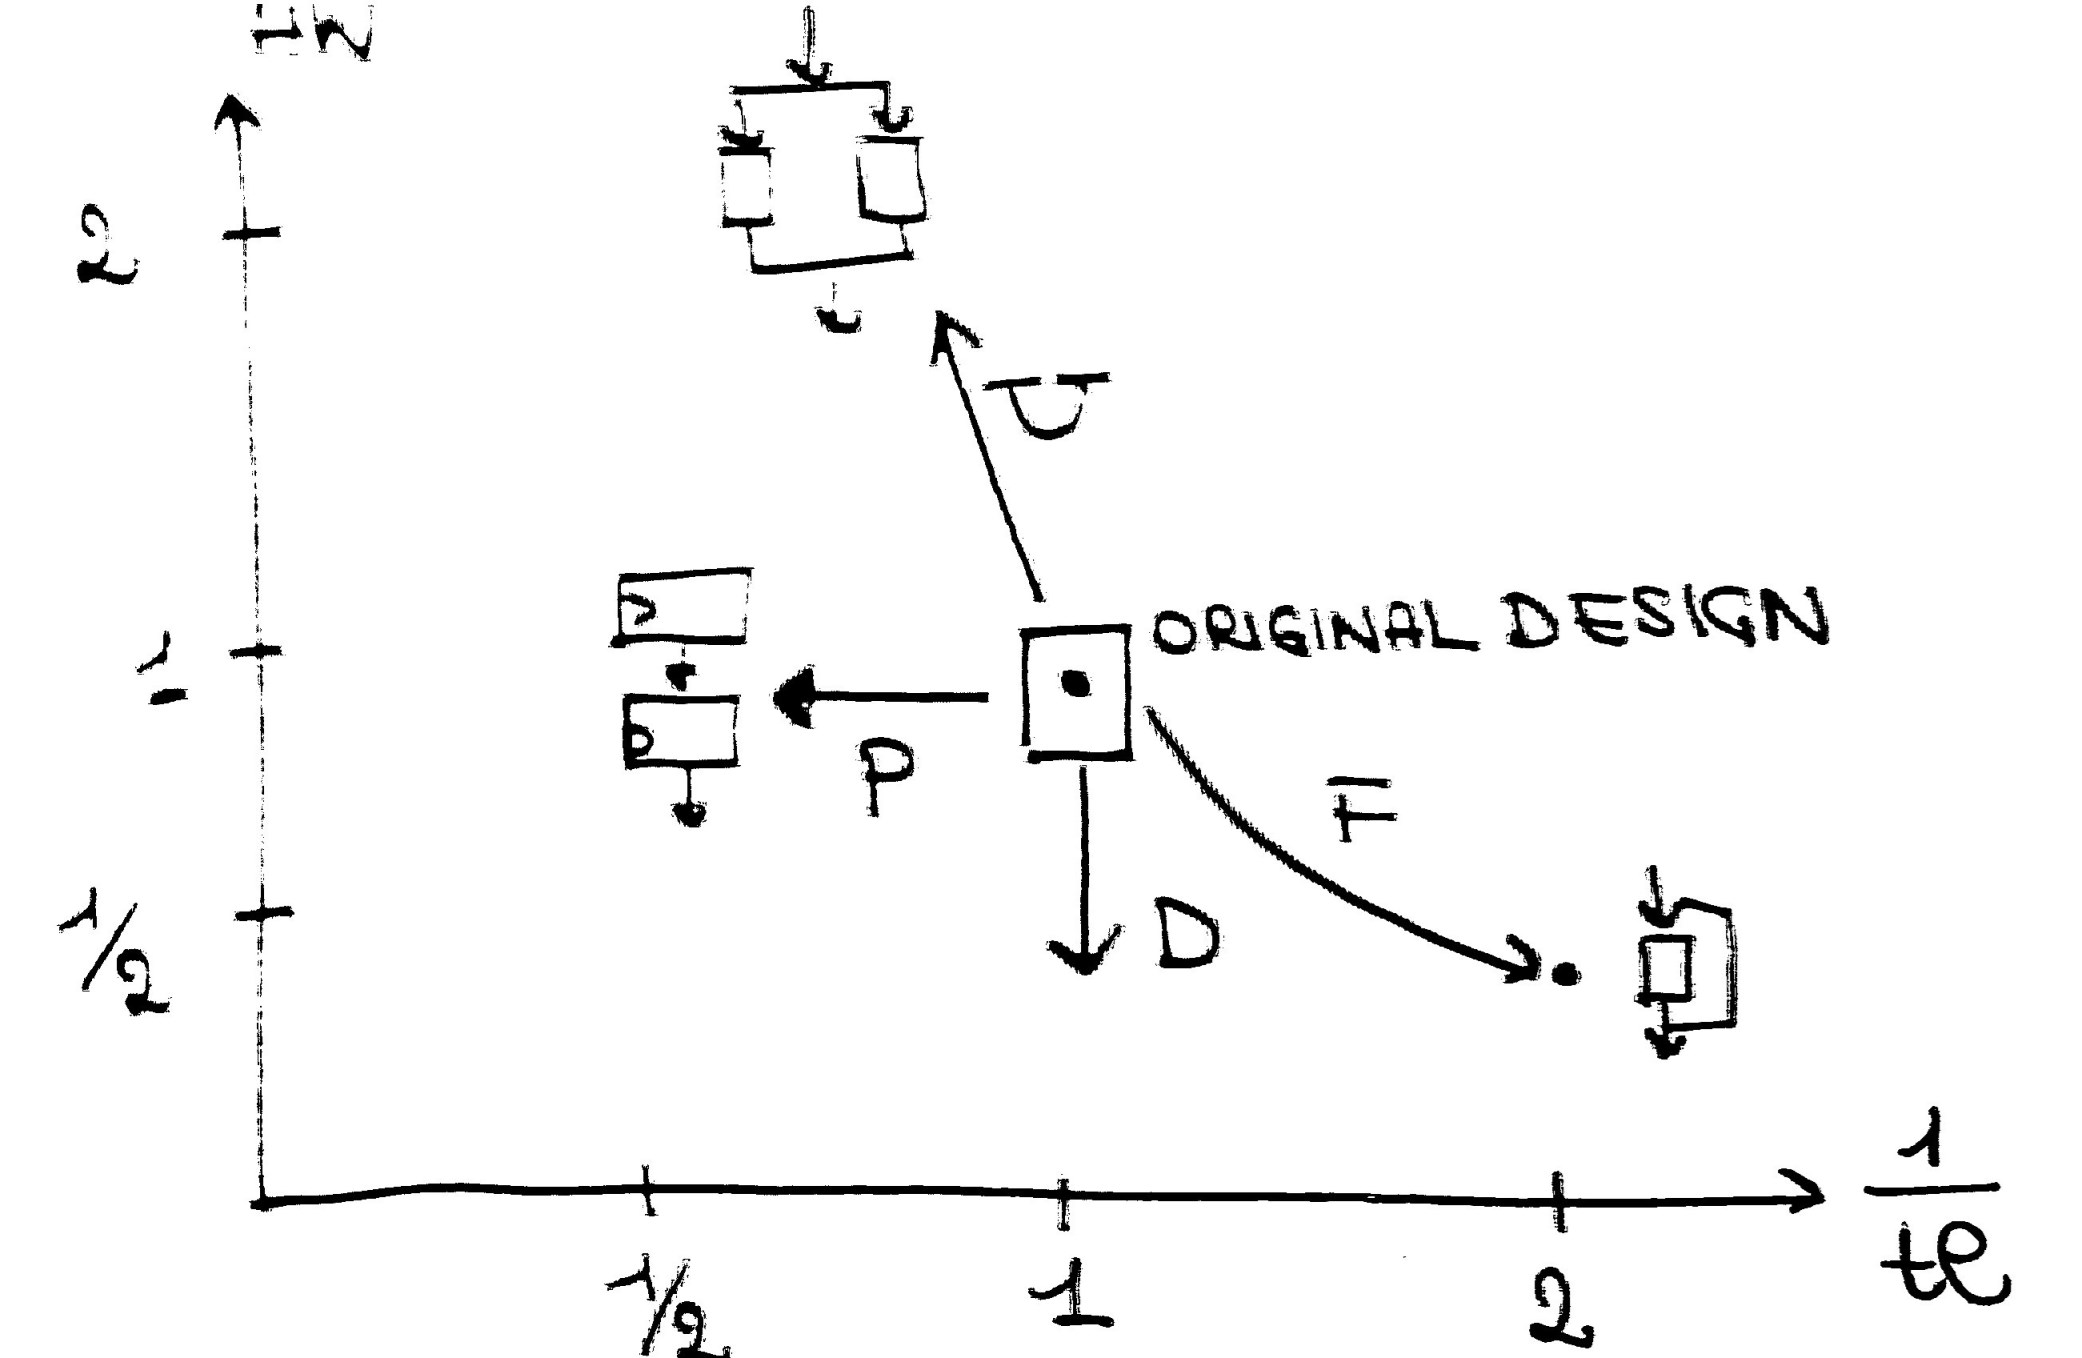
\includegraphics[width=0.7\linewidth]{img/img1/40}
\end{center}

Looking at a graph where y-axis corresponds to hardware complexity and x-axis to the the inverse of speed-up, the point corresponding to (1,1) is the single input single output stream with a direct mapping from algorithm to hardware. Applying different methods then it is possible to move this point:
\begin{itemize}
  \item Pipelining (P): ideally no extra cost but twice speed (supposing a degree of parallelism equal to 2).
  \item Unfolding(U): the cost for hardware double as the throughput.
  \item Folding(F): decrease hardware complexity but performances become worst.
\end{itemize}

Actually speedup is not the ideal one but it will saturate. A deviation from the ideal behavior is also given by the fact that we neglect the overhead hardware (multiplexer, interconnects, registers). Moreover, like in pipeline, if the split is not in the middle the gain in term of performance will not be equal to 2 (same thing for folding). Just considering the bottom part of that graph, we did not consider the direction moving down (decrease HW with almost no throughput penalty): it's called decomposition.\\

Consider a task $f$ that requires a certain amount of time and imagine that this big task can be divided into three smaller task each one equivalent to the other.

\begin{center}
  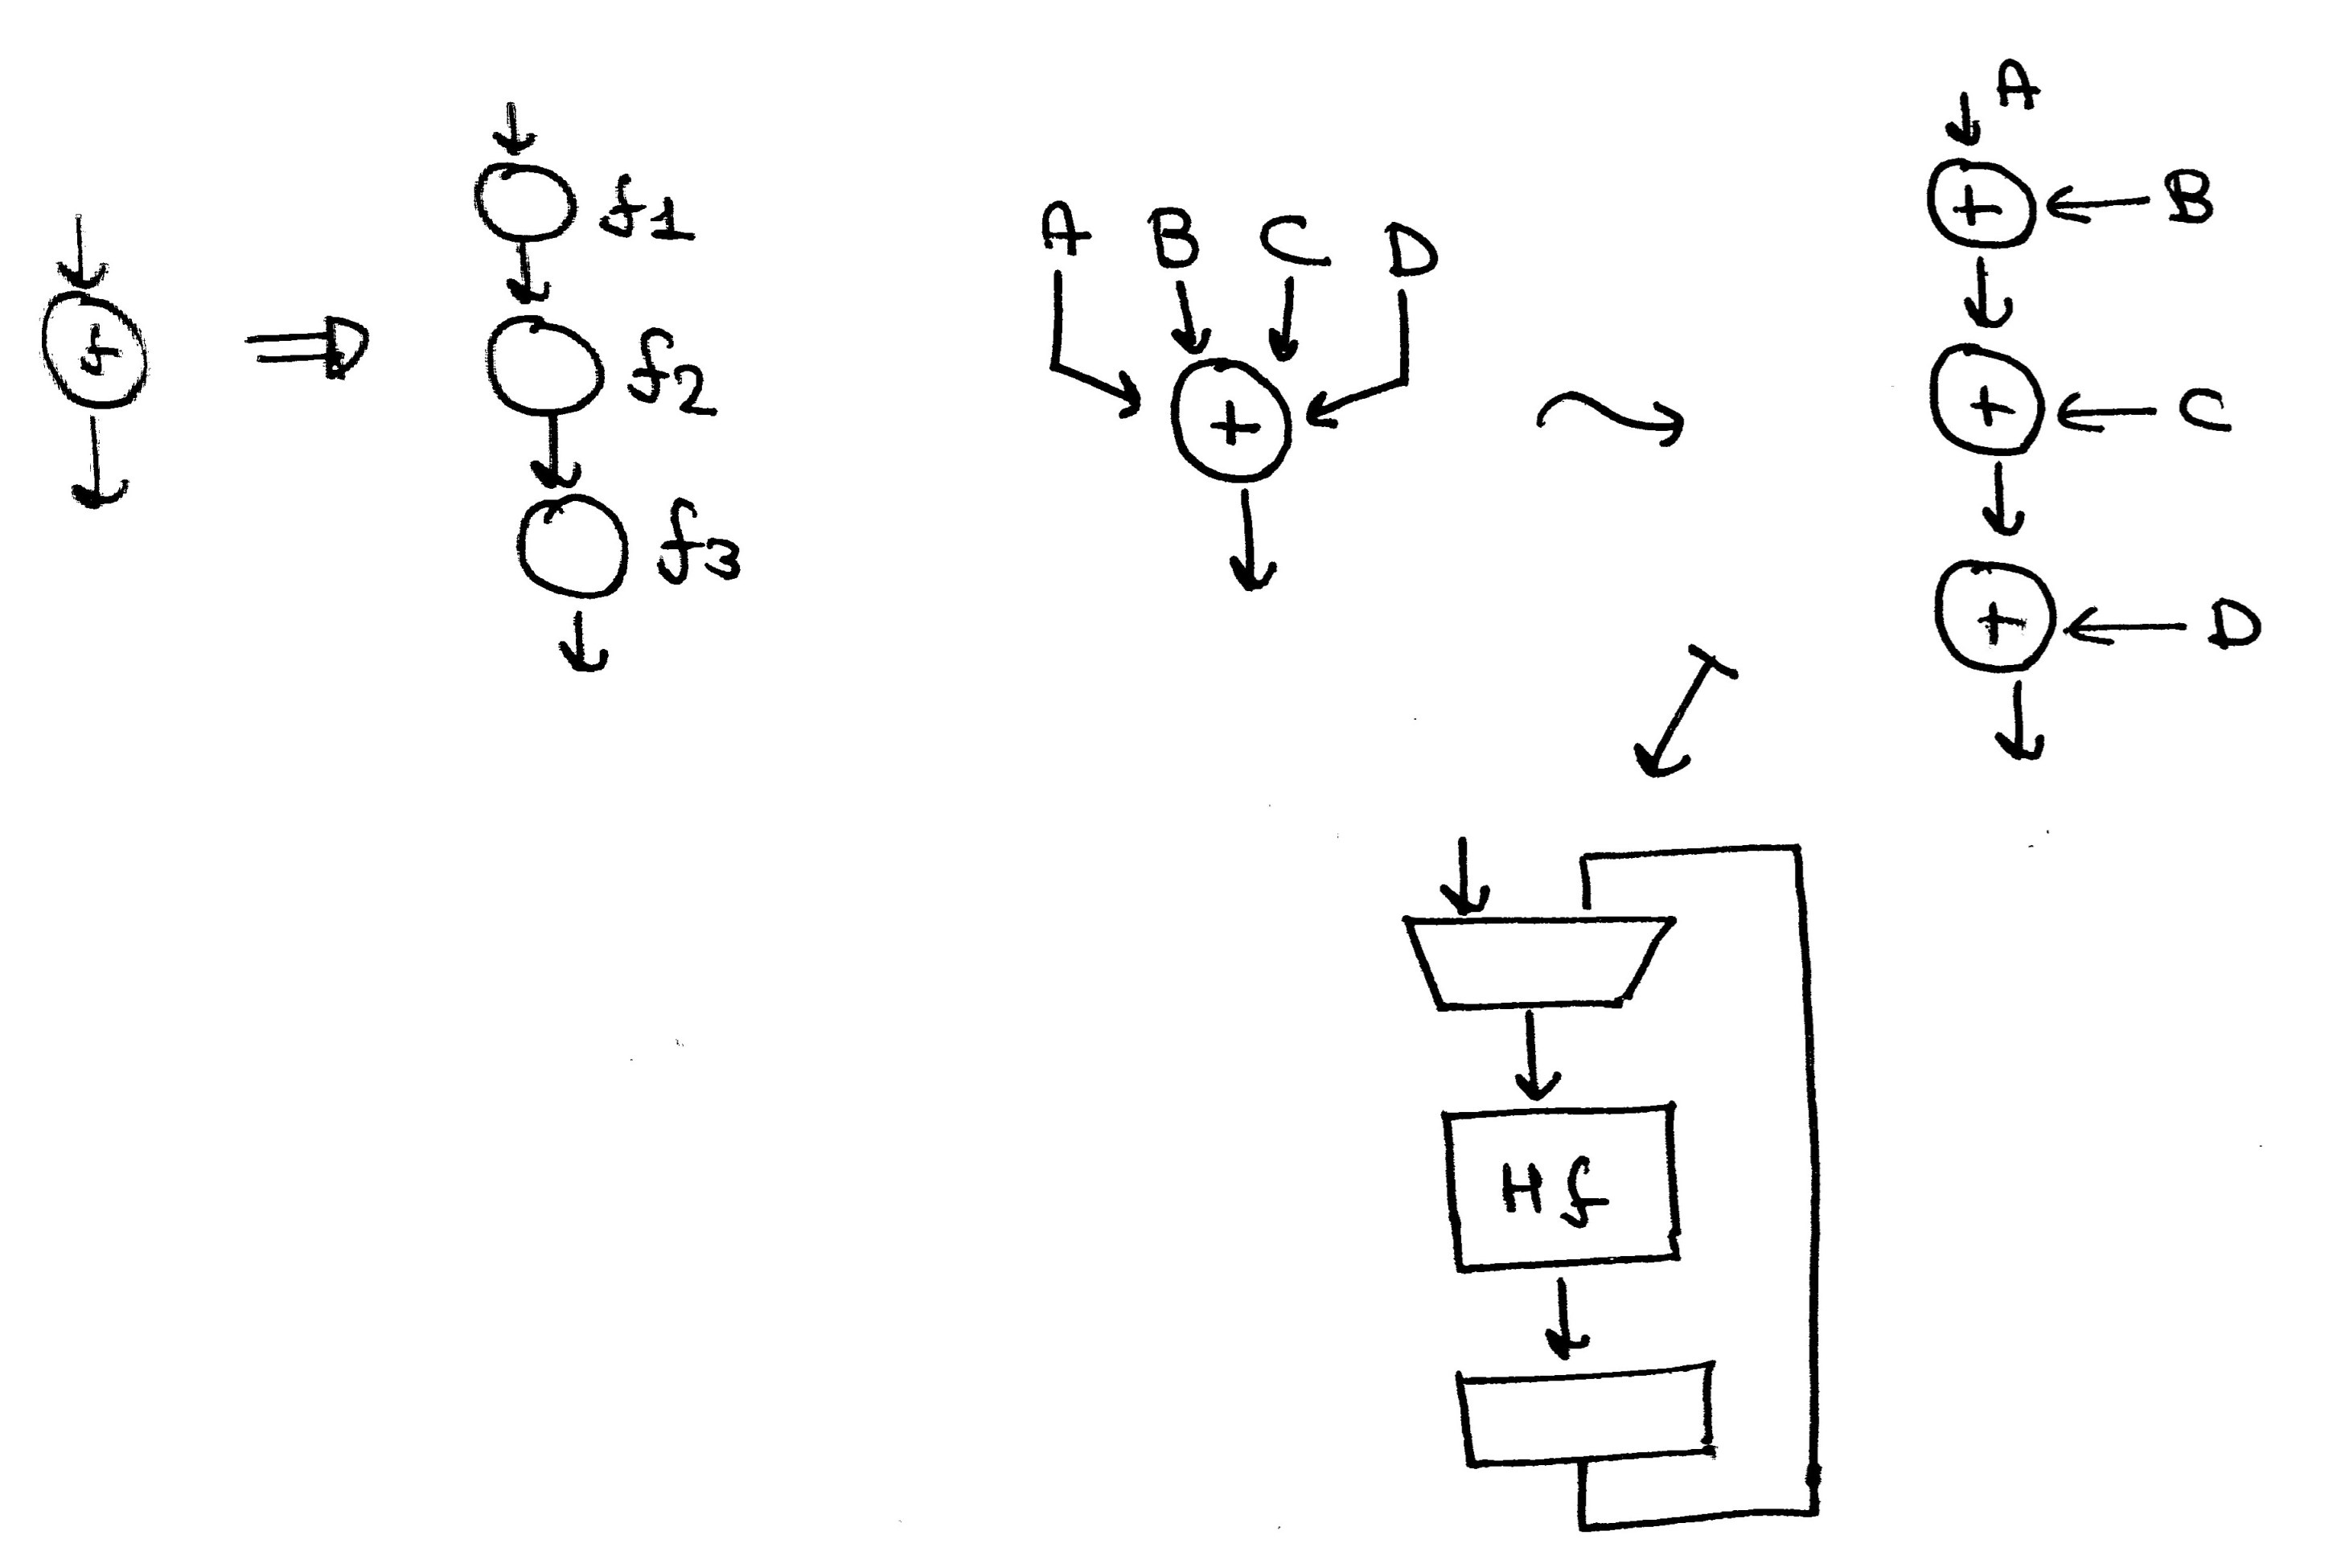
\includegraphics[width=0.7\linewidth]{img/img1/41}
\end{center}

While in case of $f$ we would need a huge adder to implement this task, if we consider $f_1$, $f_2$ and $f_3$ we can reuse a simpler hardware block to perform these three smaller task. Mapping the original algorithm into a single block $f$, this corresponds to a required time amount equal to $T_f$ and a complexity $C_f$. Applying the decomposition of order 3, the new complexity is $1/3 C_f$ and also the required time amount for each task will be one third of the previous but in this case we need three clock cycles, so:
$$T_f'= \frac{1}{3} T_f  3 = T_f$$

Applying decomposition no changes in performance occur but we obtain a reduction in hardware equal to the degree of decomposition. Again ideally (neglecting registers, multiplexer) we have no penalties in term of speed.

\section{Non universal method}
All these techniques are universal since they don't depend on particular properties of the algorithm. Other methods instead use particular properties.

\subsection{Associative property}

\begin{center}
  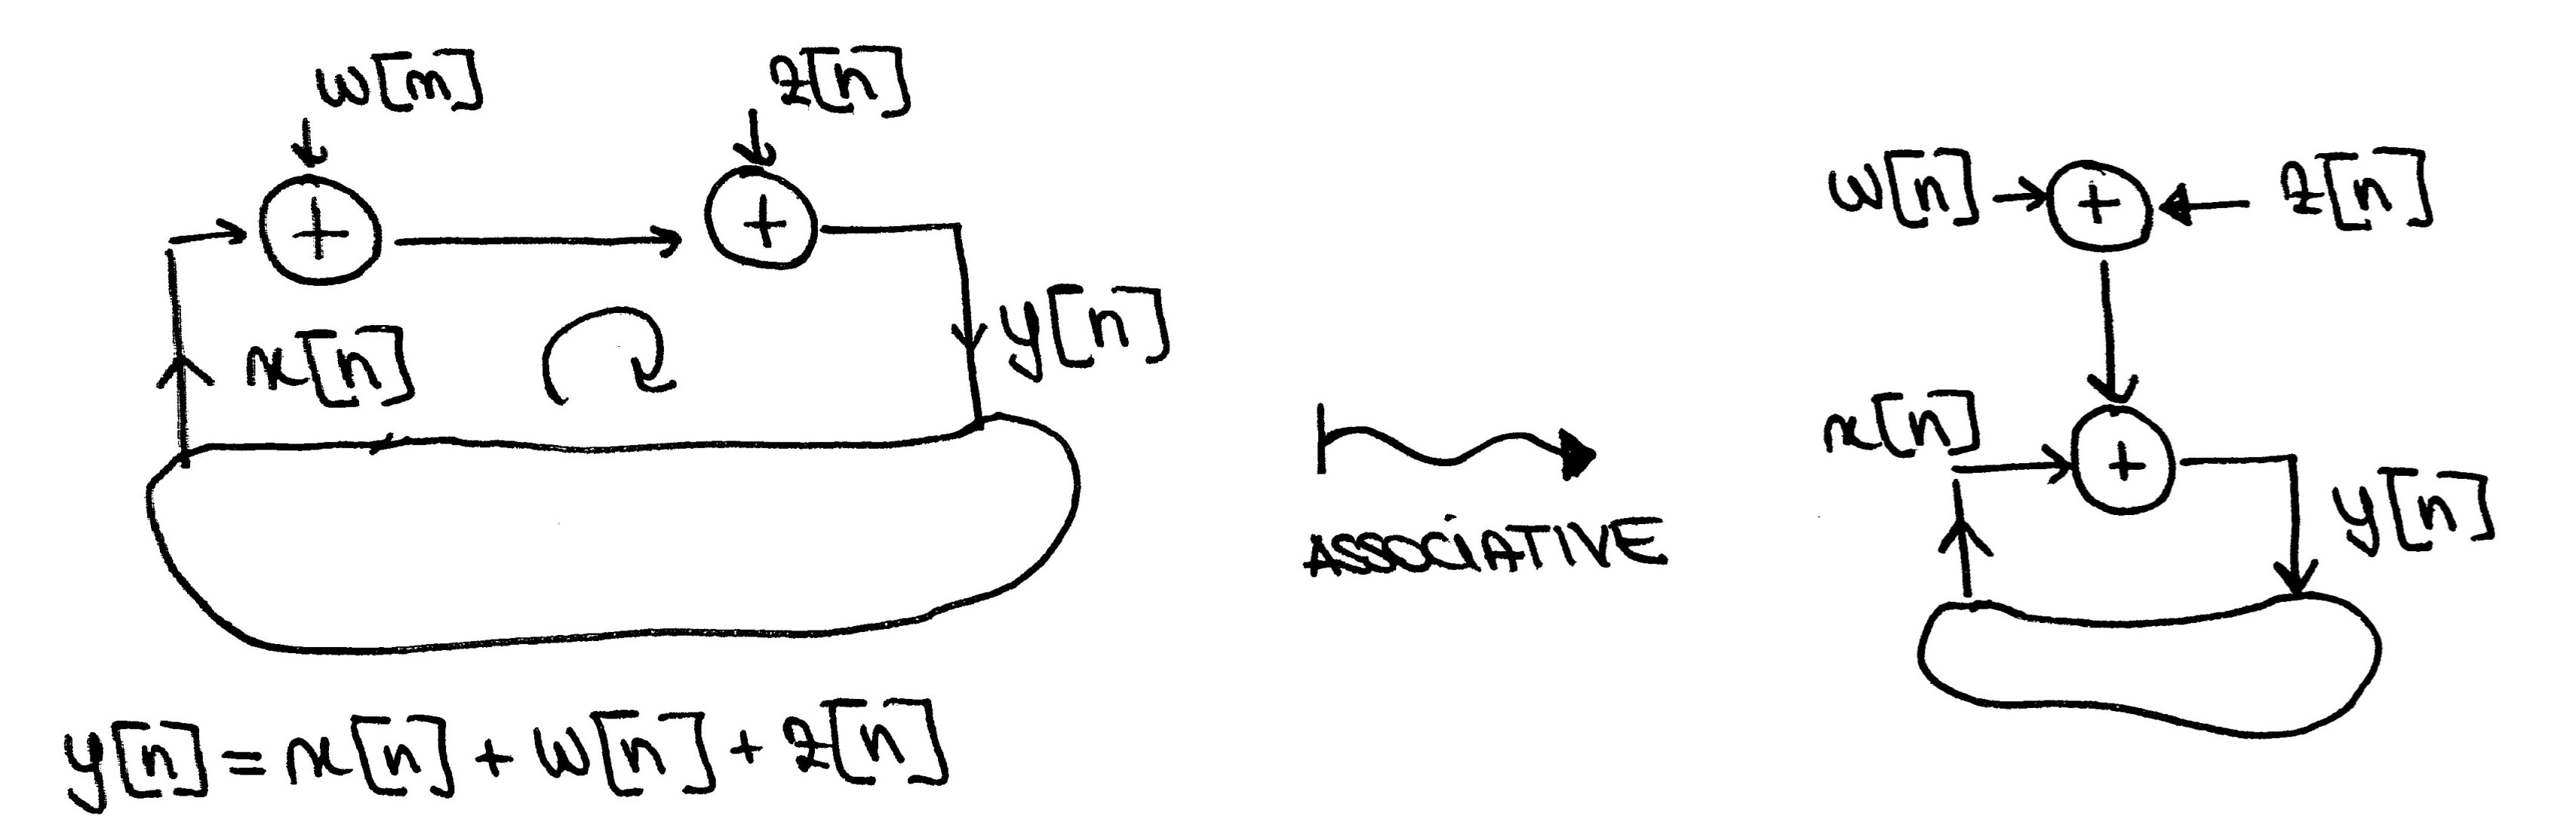
\includegraphics[width=0.7\linewidth]{img/img1/42}
\end{center}

Applying this transformation, the critical path (i.e. the path with 2 adders) will be reduced.

\subsection{Distributive property}

\begin{center}
  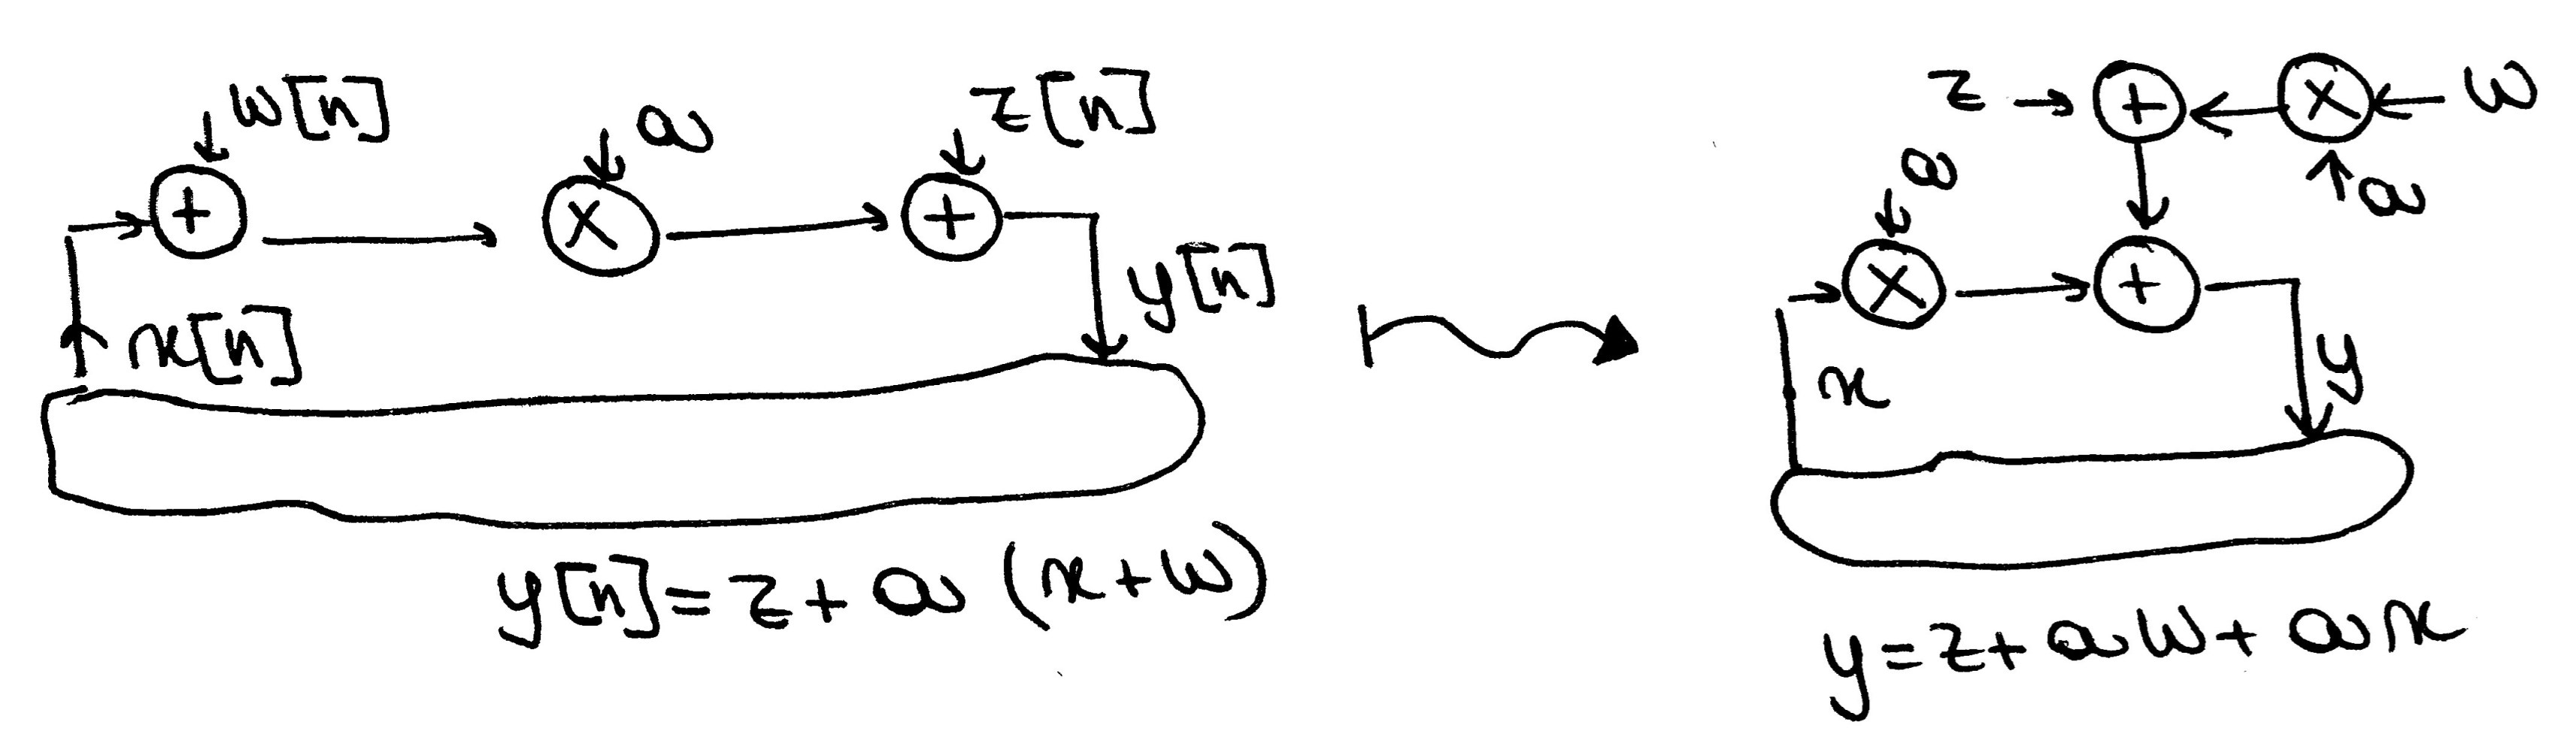
\includegraphics[width=0.7\linewidth]{img/img1/43}
\end{center}

Trying to move operators along the critical path, using distributive property we obtain a new graph resulting in a shorter critical path.

\subsection{Cascade of operations}

For instance the search for the minimum in a set of data uses the same building block having two inputs.
We want to find $m= min_i{x_i}$, so a first idea is to allocate N basic blocks, but increasing N the delay and the hardware complexity will increase linearly.
A better idea consist of a tree-like organization so the overall delay will be $log_2 (N)$.
\begin{center}
  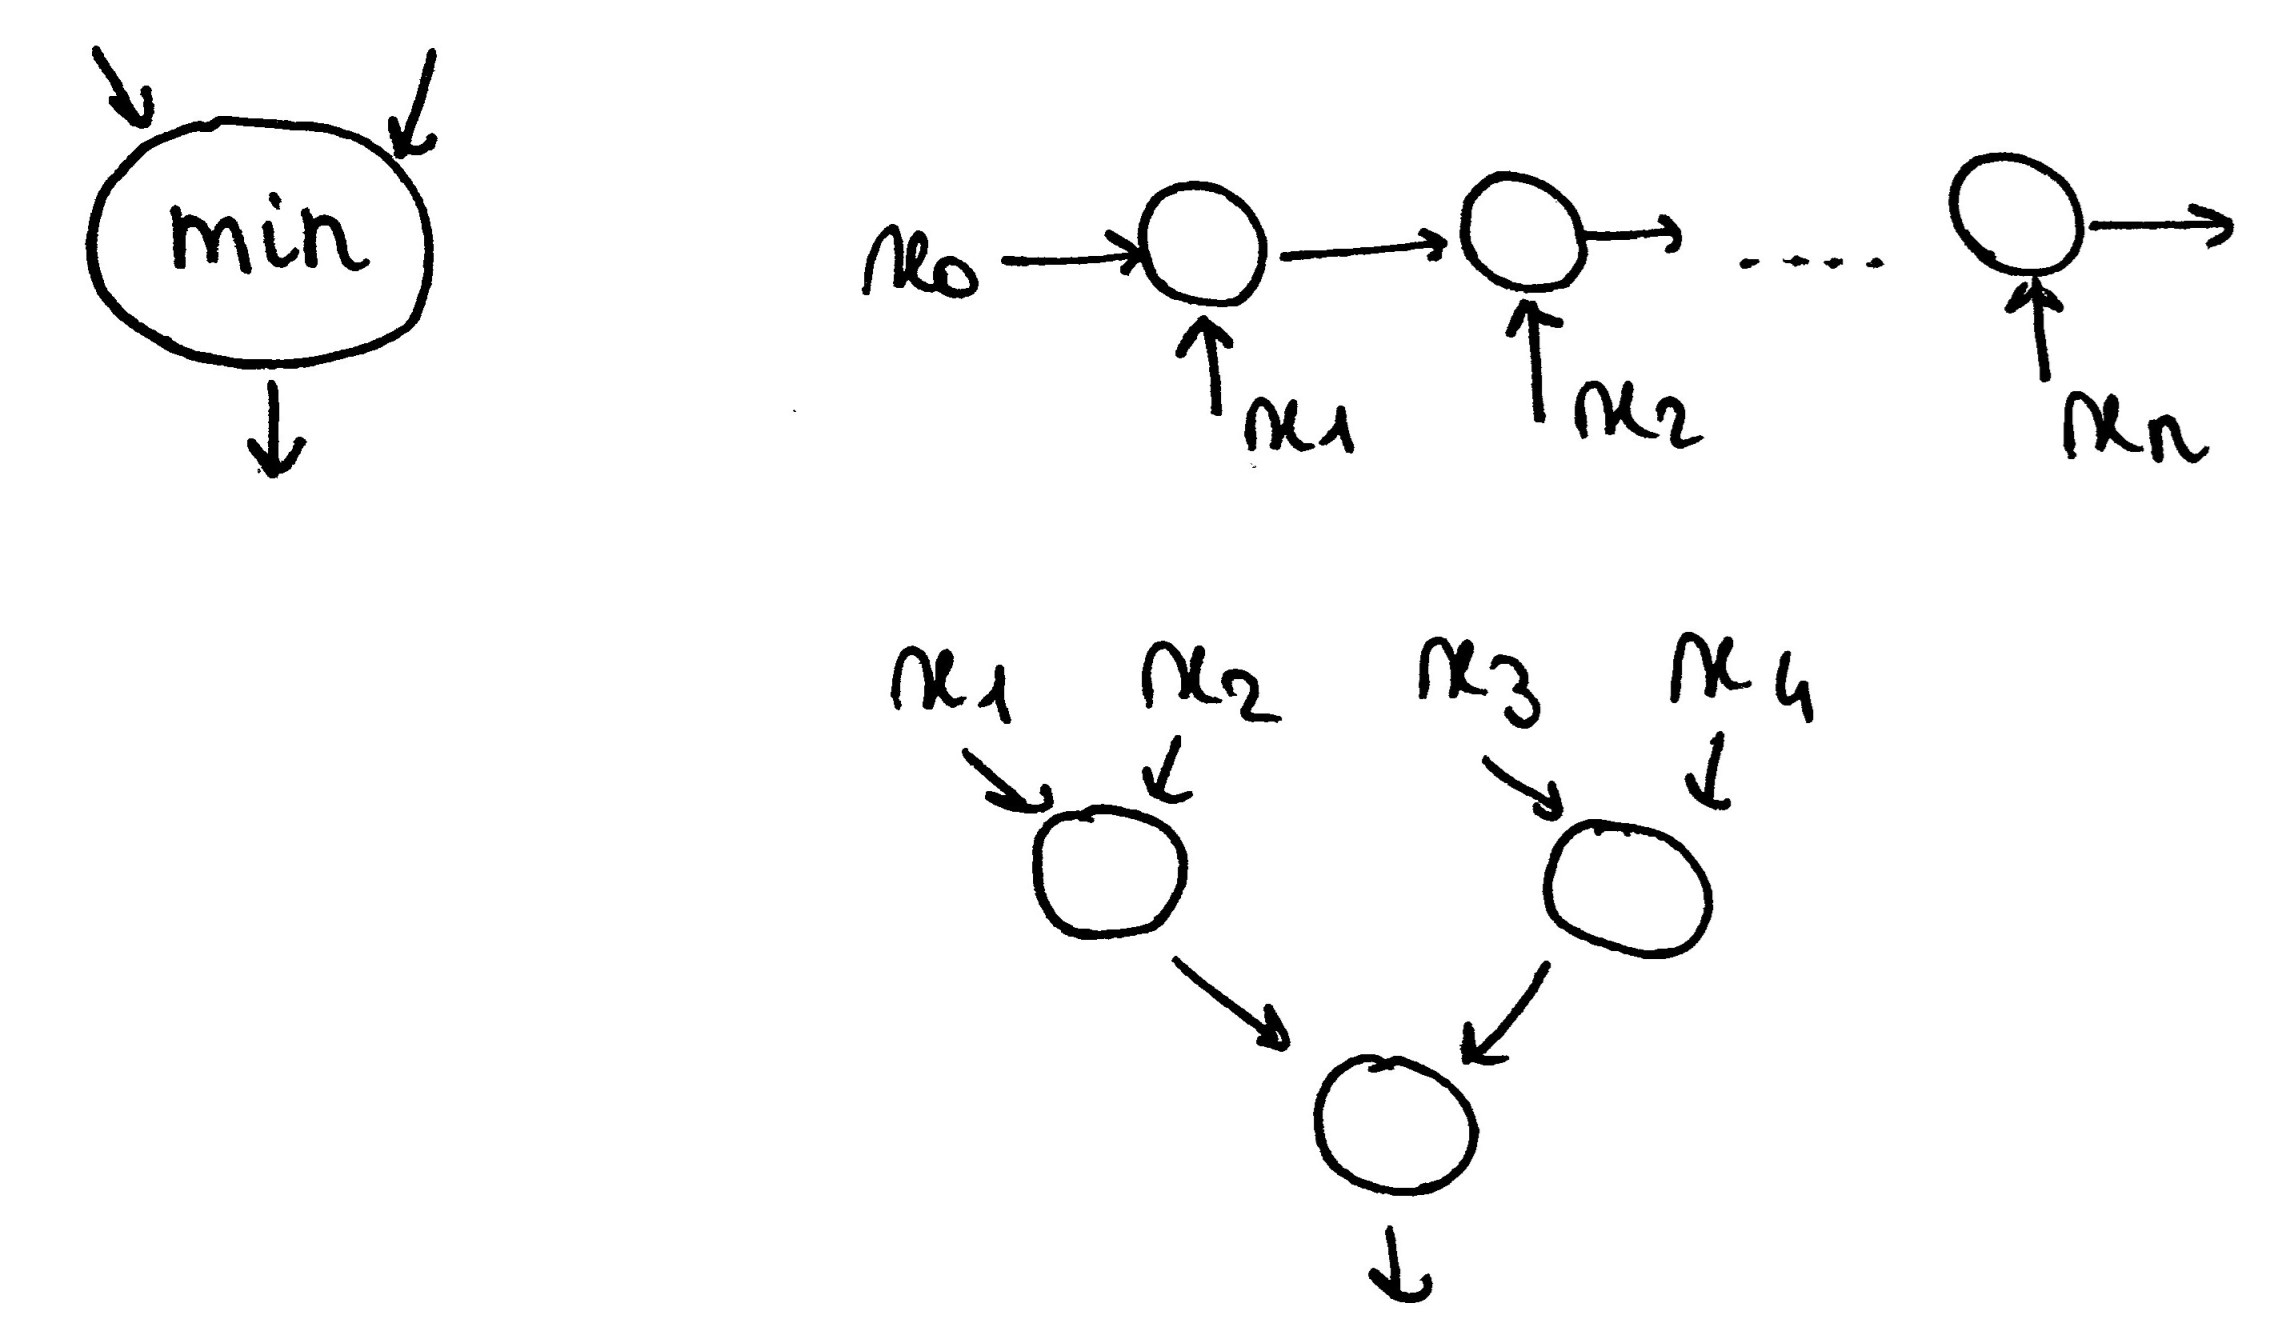
\includegraphics[width=0.7\linewidth]{img/img1/44}
\end{center}

\subsection{Look ahead method}
The typical bottleneck for a DFG are loops (we cannot apply pipelining), this method tries to resolve this problem by cutting the feedback.
An example is an IIR filter where no pipeline can be applied, $T_{cp}= T_a + T_m $ and since it's already equal to $T_{\infty}$ then we cannot improve this circuit.
Also if we try to apply unfolding, no improvement in performances will occur.

\paragraph{Analytic derivation}
Since a IIR filter is a linear system having constant coefficients, look-ahead method can be applied. Starting from the equations:
\begin{equation} \label{eq:1}
y[n]=x[n]+ay[n-1]
\end{equation}

Replacing $n$ with $n+1$:

\begin{equation}
y[n+1]=x[n+1]+ay[n]
\end{equation}

And instead of $y[n]$ place \eqref{eq:1}:
\begin{equation}
y[n+1]=x[n+1]+ax[n]+a^2y[n-1]
\end{equation}

Since the system is time invariant:
\begin{equation}
y[n]=x[n]+ax[n-1]+a^2 y[n-2]
\end{equation}

The potential advantage of this proceed can be understood looking at the new DFG:
\begin{center}
  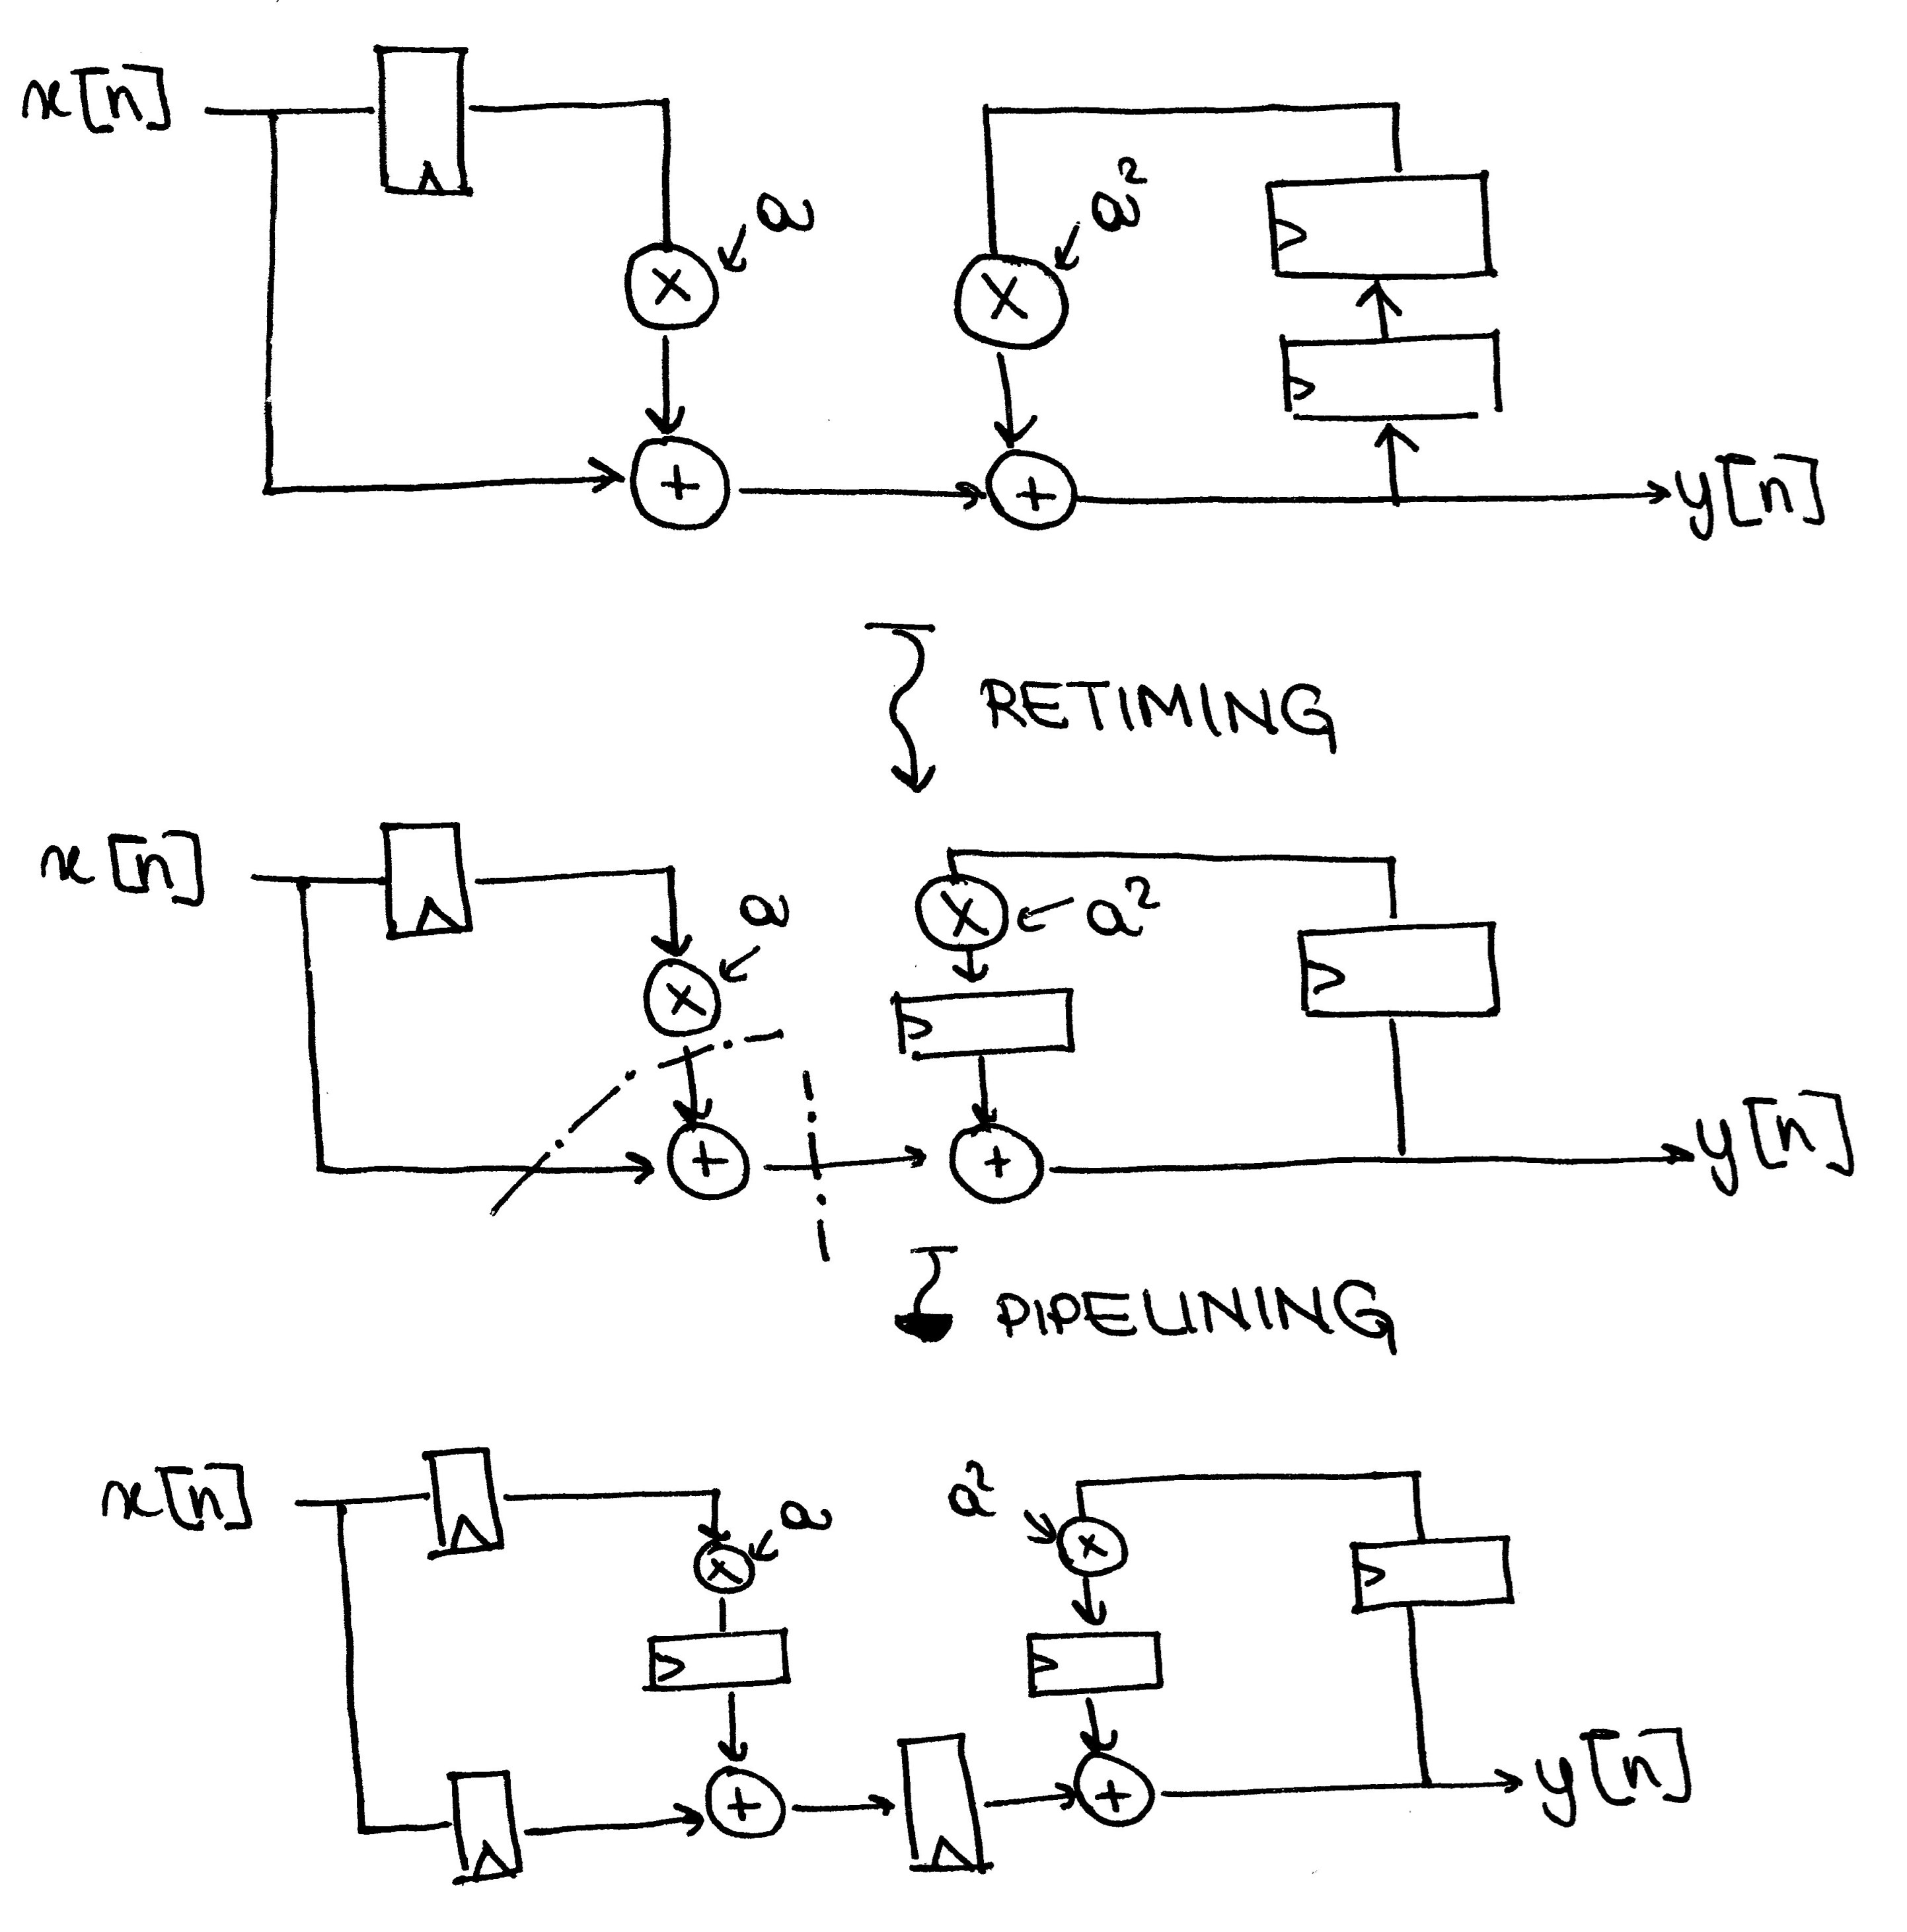
\includegraphics[width=0.7\linewidth]{img/img1/45}
\end{center}

In this new graph we have two registers together: by simply applying retiming we can move one register after and so we don't have anymore a path with both adder and multiplier one after the other. Therefore using this technique it is possible to speed up the circuit, moreover we can apply pipeling to the first part.

So applying look ahead, retiming and pipelining we obtain a $T_{cp}=T_m$ and the new loop bound is:
$$T_\infty=\frac{T_m+T_a}{2}$$

Meaning that using unfolding we can reach the optimal implementation. This method can be apply more than one time, so in the final equation we can again apply look-ahead:

\begin{eqnarray}
y[n+2]=x[n+2]+ax[n+1]+a^2 y[n]\\
y[n+2]=x[n+2]+ax[n+1]+a^2 x[n]+a^3 y[n-1]\\
y[n+2]=x[n]+ax[n-1]+a^2 x[n-1]+a^3 y[n-3]\\
\end{eqnarray}

The first part (feed-forward) becomes more difficult but with pipeline it's easy to speed up, in the second part there's a single loop with many registers: here we can apply retiming.

\begin{center}
  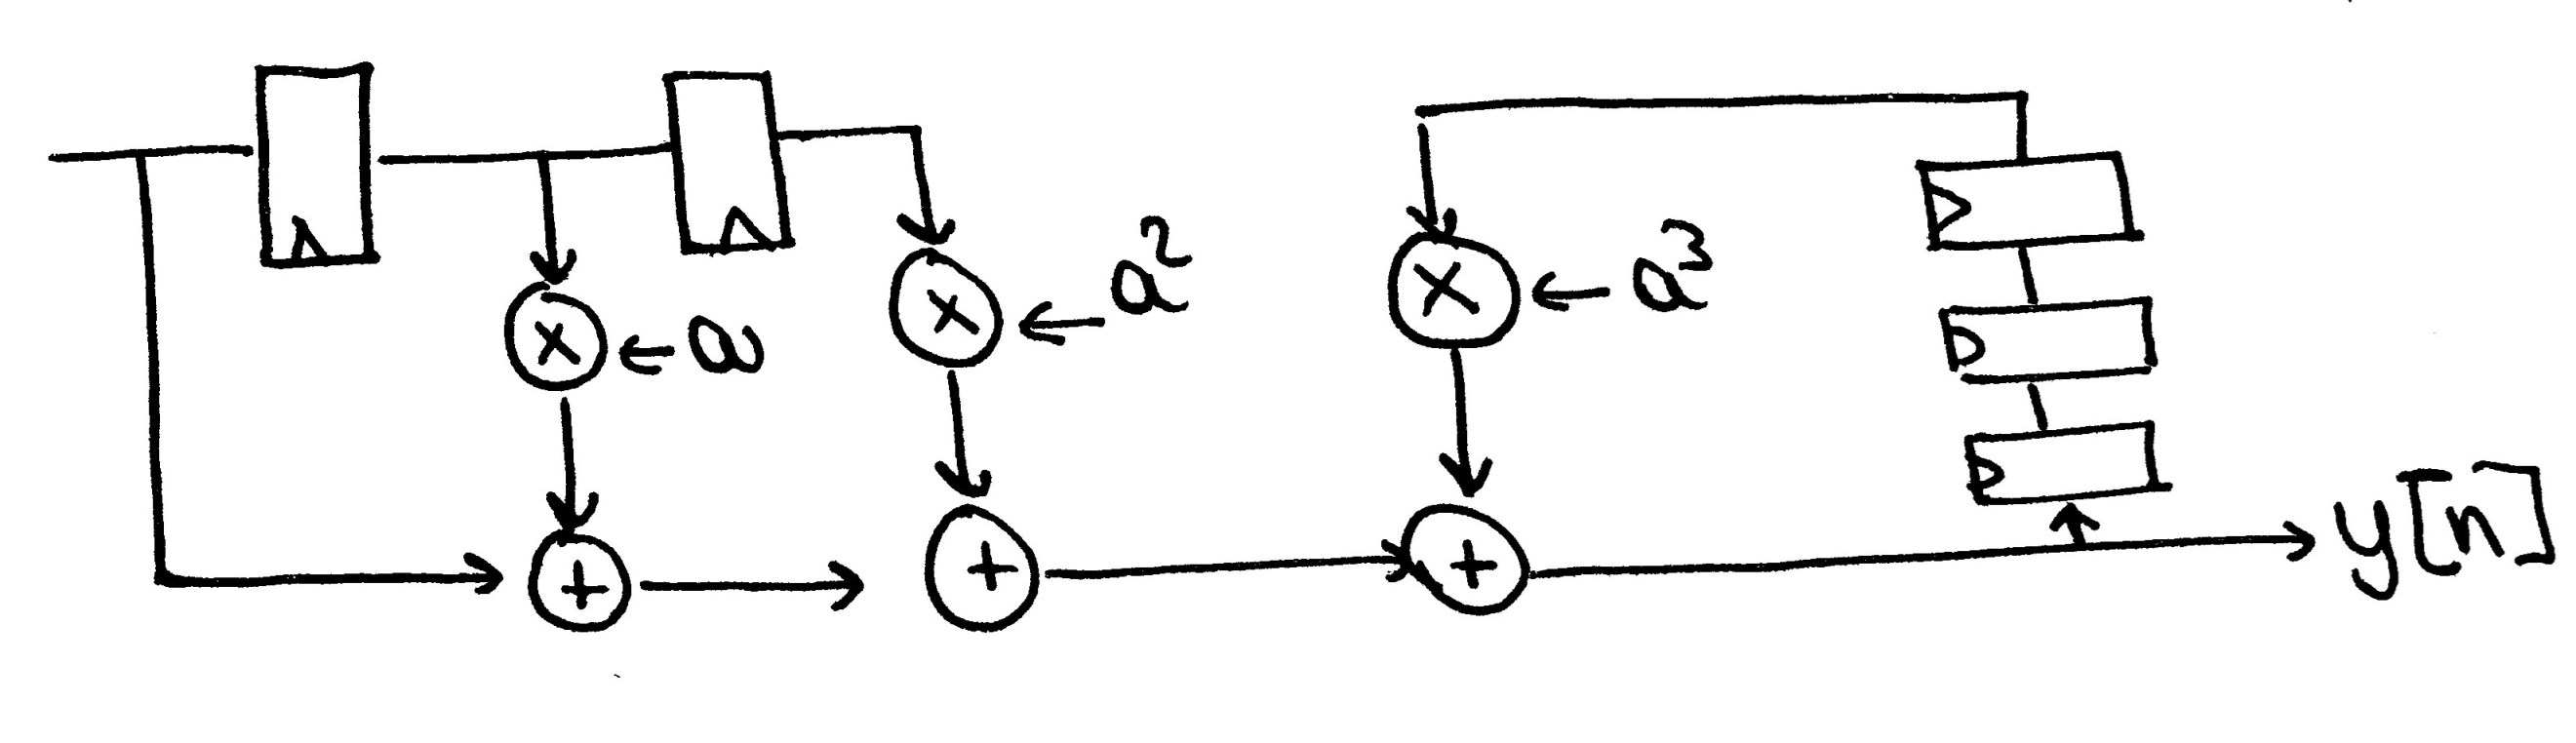
\includegraphics[width=0.7\linewidth]{img/img1/46}
\end{center}

Looking at this new DFG we have:
$$T_{\infty}=\frac{T_a+T_m}{3}$$

\paragraph{Z-domain}
In z-transform domain it is equivalent to:
\begin{eqnarray}
y[n]=x[n]+ay[n-1]\\
Y(z)=X(z)+aY(z) z^{-1}\\
\frac{Y(z)}{X(z)}= \frac{1}{1-az^{-1}}
\end{eqnarray}

We want to obtain an higher order of polynomial to have more than one register:
$$\frac{1}{1-az^{-1}} \cdot \frac{1+az^{-1}}{1+az^{-1}} = \frac{1+az^{-1}}{1+a^2 z^{-2}}$$

Leading to the same result as in time domain.

\subsection{Interleaving}
It is not an universal method, just looking at an IIR filter, although $T_{cp}=T_\infty$ we cannot improve it by using universal method.
This filter works on a stream of samples, so we can consider it as a block that is always working on a an infinite long stream. In reality data are organized in blocks or frames, so we don't have to deal with infinite length stream. One idea is to mix together samples coming from different frames: instead of applying the two frames one after the other (in sequence), the idea is to take one sample by one frame and the following from the second one. So just switching the input:

\begin{center}
  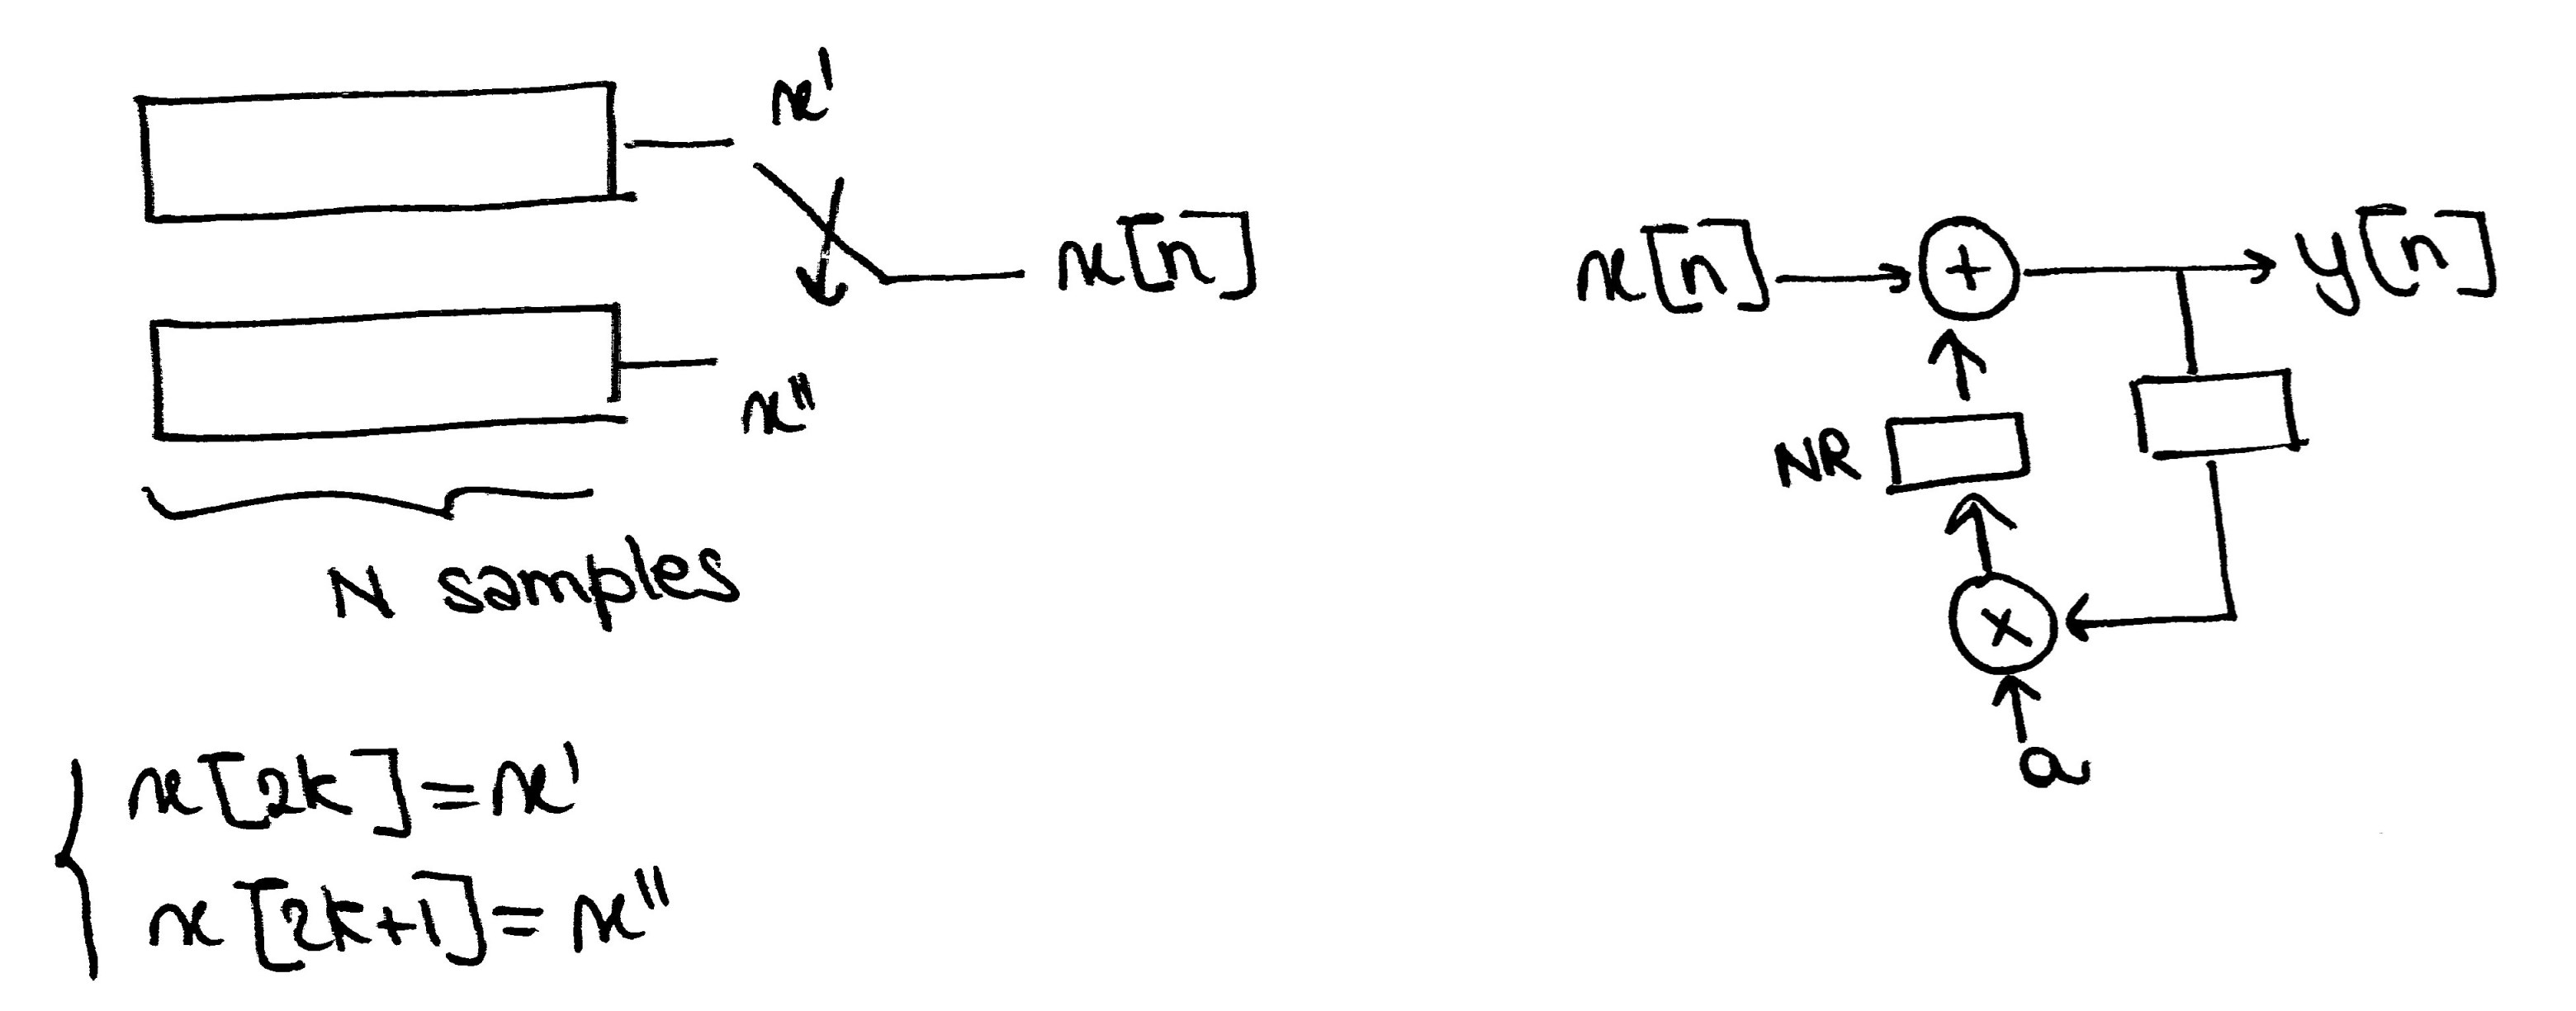
\includegraphics[width=0.7\linewidth]{img/img1/47}
\end{center}

In our filter there will be intermediate values of both two blocks: to make it works we have to insert a register to separate even from odd. It's convenient to put this register between the adder and the multiplier, in this way we obtain the new DFG and looking at the equations what we obtain is:
$$y[n]=x[n]+ay[n-2]$$

It seems to be a different filter, but just looking at the odd and even position:
\begin{eqnarray}
Even \ \rightarrow \ y[2k]=x[2k]+ay[2(k-1)]
Odd \ \rightarrow \ y[2k+1]=x[2k+1]+ay[2(k-1)+1]
\end{eqnarray}

Meaning that it's working properly. During the computation the filter is working on two streams in parallel. Assuming an interleaving of factor equal to 3, we suppose to have 3 incoming streams. This is very powerful since we can achieve higher frequency at the cost of just a single register. This is not an universal method because we need to assume that the processing is working on frames.\\

The drawback is latency: to complete the process of a single stream we need $2N$ clock cycles and also more memory, however in a lot of hardware application latency is not a critical aspect.
